\chapter{Daten der empirischen Untersuchung} % (fold)
\label{cha:daten_der_empirischen_untersuchung}

Die Darstellung der erhobenen Rohdaten der empirischen Untersuchung und deren detaillierte Auswertung würden an dieser Stelle den Rahmen der Arbeit sprengen. Durch die große Anzahl an Videoaufnahmen, die insgesamt etwa XY \gls{GB} an Platzbedarf einnehmen, ist auch die Beilage eines Datenträgers nicht möglich. 

Die Rohdaten, die durchgeführten Auswertungen und Transkripte sowie die Skripte der statistischen Tests mit der Software R können via eMail unter

\begin{center} stefan@oppl.info \end{center}

angefordert werden. 

\section{Verfügbare Rohdaten} % (fold)
\label{sec:verfügbare_rohdaten}

Zu den Untersuchungen stehen im Einzelnen folgende Rohdaten zur Verfügung:
\begin{itemize}
	\item Evaluierungsblock 1 (siehe auch \citep{Bohninger10})
		\begin{itemize}
			\item Videoaufnahmen der Modellbildung (Detailansicht der Modellierungsoberfläche)
			\item Fotos der finalen Versionen der erstellten Modelle
		\end{itemize}
	\item Evaluierungsblock 2
		\begin{itemize}
			\item Videoaufnahmen der Modellbildung aus jeweils 2 Perspektiven (Gesamtübersicht inkl. Personen sowie Detailansicht der Modellierungsoberfläche)
			\item Fotos bzw. Graphische Abbildungen der finalen Versionen der erstellten Modelle
		\end{itemize}
	\item Evaluierungsblock 3
		\begin{itemize}
			\item Videoaufnahmen der Modellbildung aus jeweils 2 Perspektiven (Gesamtübersicht inkl. Personen sowie Detailansicht der Modellierungsoberfläche)
			\item Graphische Abbildungen der finalen Versionen der erstellten Modelle
		\end{itemize}
	\item Evaluierungsblock 4 (siehe auch \citep{Wahlmuller10})
		\begin{itemize}
			\item Videoaufnahmen der Modellbildung können aus Gründen der Schutzes unternehmensinterner Information auf diesem Wege nicht weitergegeben werden. Etwaige Anfragen sind an Patrick Wahlmüller (Kontaktdaten in \citep{Wahlmuller10}) zu richten.
			\item Graphische Abbildungen der finalen Versionen der erstellten Modelle
		\end{itemize}
	\item Evaluierungsblock 5 (siehe auch \citep{Bindreiter10})
		\begin{itemize}
			\item Videoaufnahmen der Modellbildung mittels CMapTools und am Modellierungstisch aus jeweils 2 Perspektiven (Gesamtübersicht inkl. Personen sowie Detailansicht der Modellierungsoberfläche)
			\item Graphische Abbildungen der finalen Versionen der erstellten Modelle
			\item Als XML exportierte Repräsentationen der mit CMapTools erstellten Modelle (inkl. Modellierungshistorie)
			\item Fragebogen 
		\end{itemize}
\end{itemize}

% section verfügbare_rohdaten (end)

\section{Durchgeführte Auswertungen} % (fold)
\label{sec:durchgeführte_auswertungen}

Zu den Untersuchungen wurden folgende Auswertungen durchgeführt und archiviert. Die einzelnen Auswertungsmethoden sind auf den folgenden Seiten näher beschrieben.

\begin{itemize}
	\item Evaluierungsblock 1 (siehe auch \citep{Bohninger10})
		\begin{itemize}
			\item Überblicksauswertung aller Anwendungen und Modelle
			\item  
		\end{itemize}
	\item Evaluierungsblock 2
		\begin{itemize}
			\item Überblicksauswertung aller Anwendungen und Modelle
			\item Interaktionsanalyse aller Anwendungen
		\end{itemize}
	\item Evaluierungsblock 3
		\begin{itemize}
			\item Überblicksauswertung aller Anwendungen und Modelle
			\item Interaktionsanalyse aller Anwendungen
		\end{itemize}
	\item Evaluierungsblock 4 (siehe auch \citep{Wahlmuller10})
		\begin{itemize}
			\item Überblicksauswertung aller Anwendungen und Modelle
			\item Interaktionsanalyse aller Anwendungen
		\end{itemize}
	\item Evaluierungsblock 5 (siehe auch \citep{Bindreiter10})
		\begin{itemize}
			\item Überblicksauswertung aller Anwendungen und Modelle
			\item Interaktionsanalyse aller Anwendungen
		\end{itemize}
\end{itemize}

\subsection{Überblicksauswertung}

Die Überblicksauswertung fasst die wesentlichen Eigenschaften des in einer Anwendung erstellten Modells sowie die während der Erstellung aufgetretenen Ereignisse zusammen. Die Daten wurden in Form einer Openoffice-Tabelle aufbereitet und stehen als \gls{ODF}-Dateien zur Verfügung. Sie dienen als Grundlage aller weiteren deskriptiven und schließenden statistischen Auswertungen.

Die konkrete Ausgestaltung der Tabelle variiert je nach Evaluierungsblock (abhängig von der durchgeführten Modellierungsaufgabe und der im Werkzeug implementierten Funktionalität) leicht, in Abbildung \ref{fig:img_AnhangEmpirie_raster} ist der Raster aus Evaluierungsblock 5 dargestellt, in dem die höchste Anzahl von Merkmalen erhoben wurden.

\begin{figure}[htbp]
	\centering
		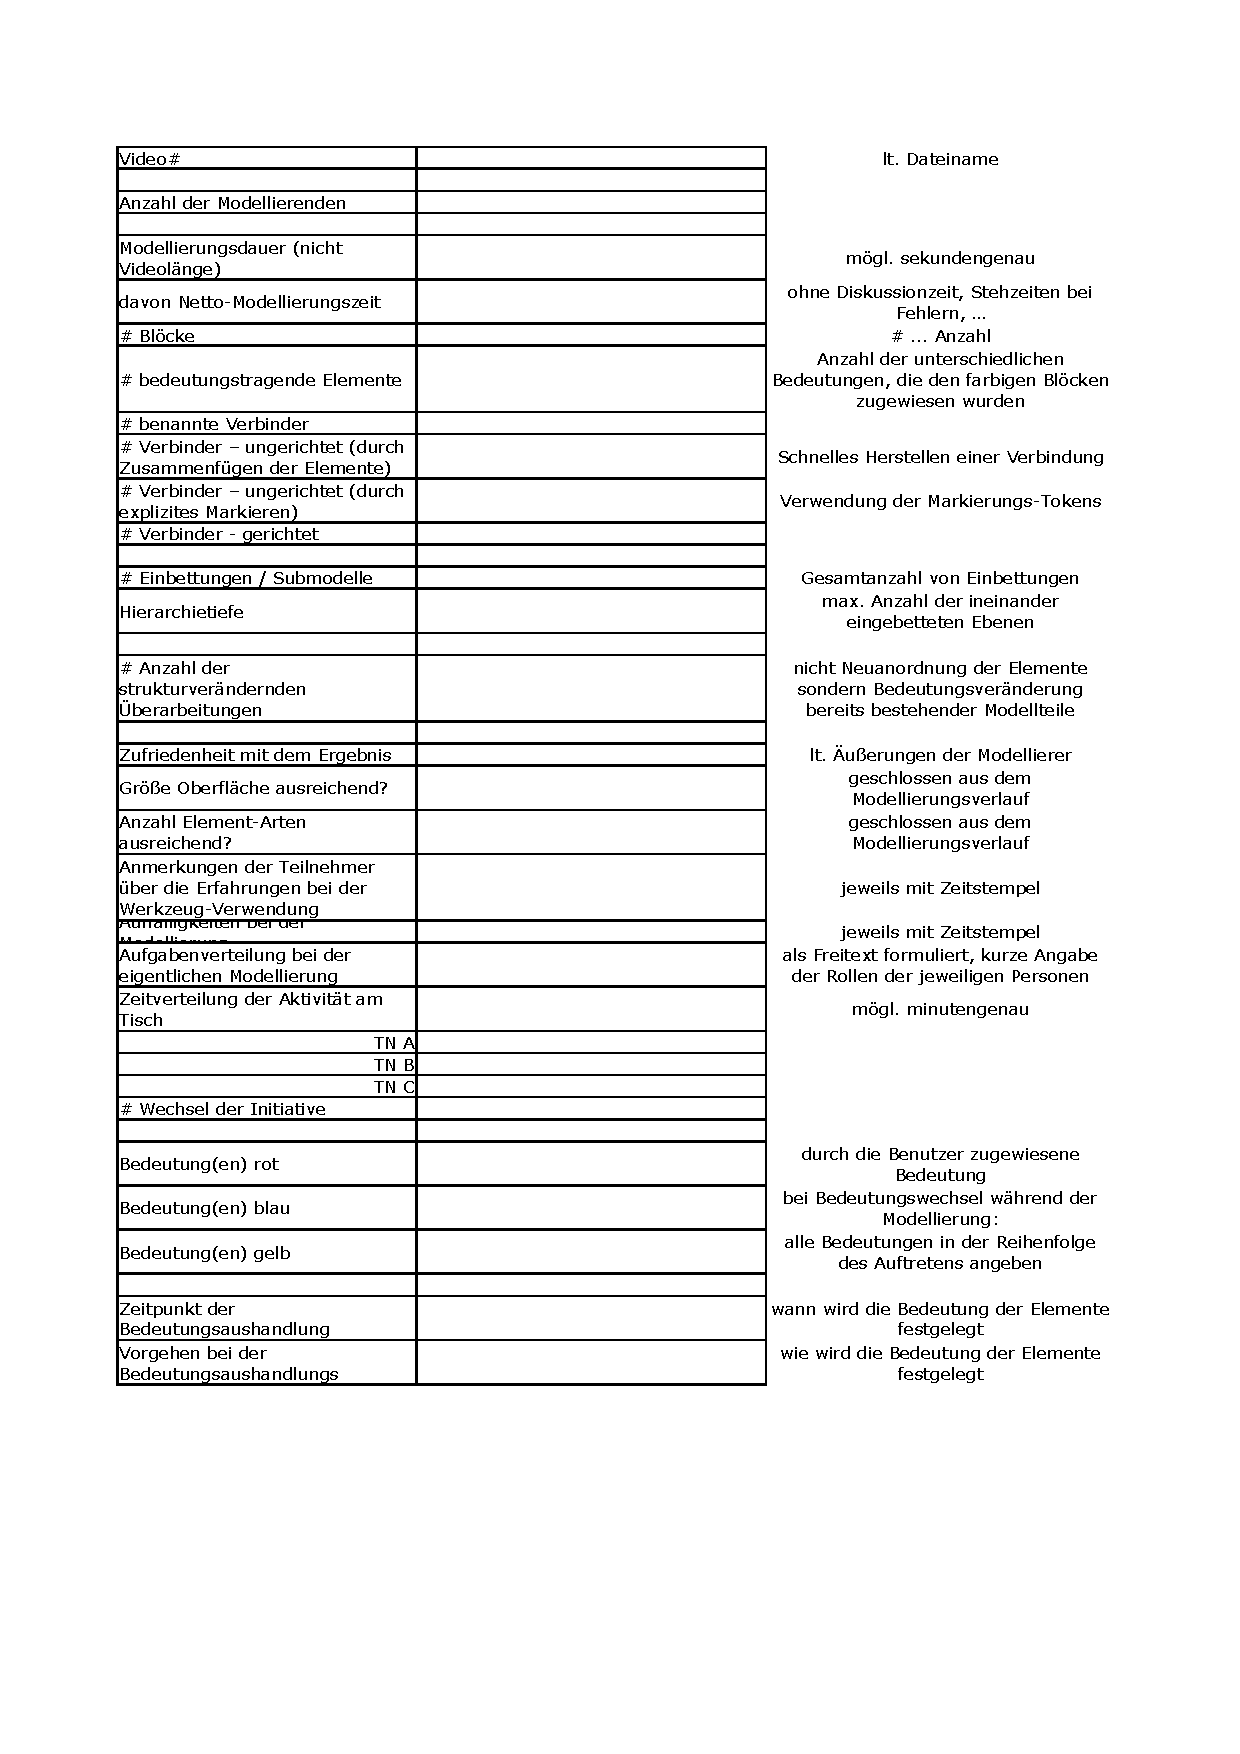
\includegraphics[width=0.9\textwidth]{img/AnhangEmpirie/raster.pdf}
	\caption{Raster der Überblicksauswertung}
	\label{fig:img_AnhangEmpirie_raster}
\end{figure}

Die Befüllung der Raster erfolgte auf Basis der angefertigten Video-Aufnahmen der Werkzeuganwendungen. In den Blöcken 3 und 5 wurden die Raster redundant unabhängig voneinander von jeweils zwei Personen befüllt. Sofern Abweichungen bei der Auswertung der quantitativen Parameter festgestellt wurden, wurde das jeweilige Merkmal durch eine dritte Person geprüft und ggf. entsprechend korrigiert. In den Blöcken 1, 2 und 4 standen nicht ausreichend personelle Ressourcen für eine redundante Auswertung zur Verfügung.

\subsection{Interaktionsanalyse}

Die Interaktionsanalyse wurde wie in Abschnitt \ref{sub:interaktionsanalyse} beschrieben durchgeführt und dokumentiert. Die Dokumentation erfolgte in Textdokumenten, die als \gls{ODF}-Dateien zur Verfügung stehen.

In den Evaluierungsblöcken 3 und 5 wurde die Interaktionsanalyse für jede Werkzeuganwendung von zwei Personen redundant durchgeführt. In den Blöcken 2 und 4 standen die personellen Ressourcen für eine redundante Auswertung nicht zur Verfügung. In den Fällen, in denen redundant ausgewertet wurde, wurden Transkripte, die nur von einer der auswertenden Personen erfasst wurden, von einer dritten Person geprüft und bestätigt bzw. verworfen.

% section durchgeführte_auswertungen (end)

\section{Verwendete Fragebögen} % (fold)
\label{sec:frageboegen}

Bei der Durchführung der Evaluierungsblöcke 1, 4 und 5 wurden zusätzlich zu den direkt aus der Modellbildung erhobenen Daten auch Benutzerbefragungen mittels Fragebögen durchgefürht. Im Folgenden sind für jeden Evaluierungsblock die verwendeten Fragebögen angeführt. Zusätzlich werden die Fragebögen hinsichlich ihrer Relevanz für die untersuchten Hypothesen (siehe Kapitel \ref{cha:eval_werkzeug} bis \ref{cha:eval_aw}) eingeordnet. Die Auswertungen der ausgefüllten Fragebögen sind in digitaler Form detailliert (siehe Abschnitt \ref{sec:verfügbare_rohdaten}) bzw. aggregiert (siehe Abschnitt \ref{sec:durchgeführte_auswertungen}) in digitaler Form verfügbar.


\fboxrule0.4mm
\fboxsep0.1mm
\clearpage
\subsection{Fragebögen aus Evaluierungsblock 1}
\label{sub:fb_eval1}

Die Abbildungen \ref{fig:img_AnhangEmpirie_fb1_1-01} bis \ref{fig:img_AnhangEmpirie_fb1_1-03} zeigen den in Evaluierungsblock 1 verwendeten Fragebogen für die Modellierenden. Die Abbildungen \ref{fig:img_AnhangEmpirie_fb1_2-01} bis \ref{fig:img_AnhangEmpirie_fb1_2-02} zeigen den in Evaluierungsblock 1 verwendeten Fragebogen für die interpretierenden Teilnehmer. Abbildung \ref{fig:img_AnhangEmpirie_fb1_3-01} zeigt den Fragebogen bezüglich der Korrektheit der Interpretation, der durch die Modellierenden ausgefüllt wurde. Abbildung \ref{fig:img_AnhangEmpirie_fb1_4-01} zeigt den Fragebogen zur Erhebung der Modellierungsvorkenntnisse. Dieser Fragebogen wurde von allen Teilnehmern ausgefüllt. Der Aufbau der Fragebögen wurde von \cite{Bohninger10} detailliert beschrieben und begründet.

\begin{figure}[htbp]
	\centering
	\fbox{%
		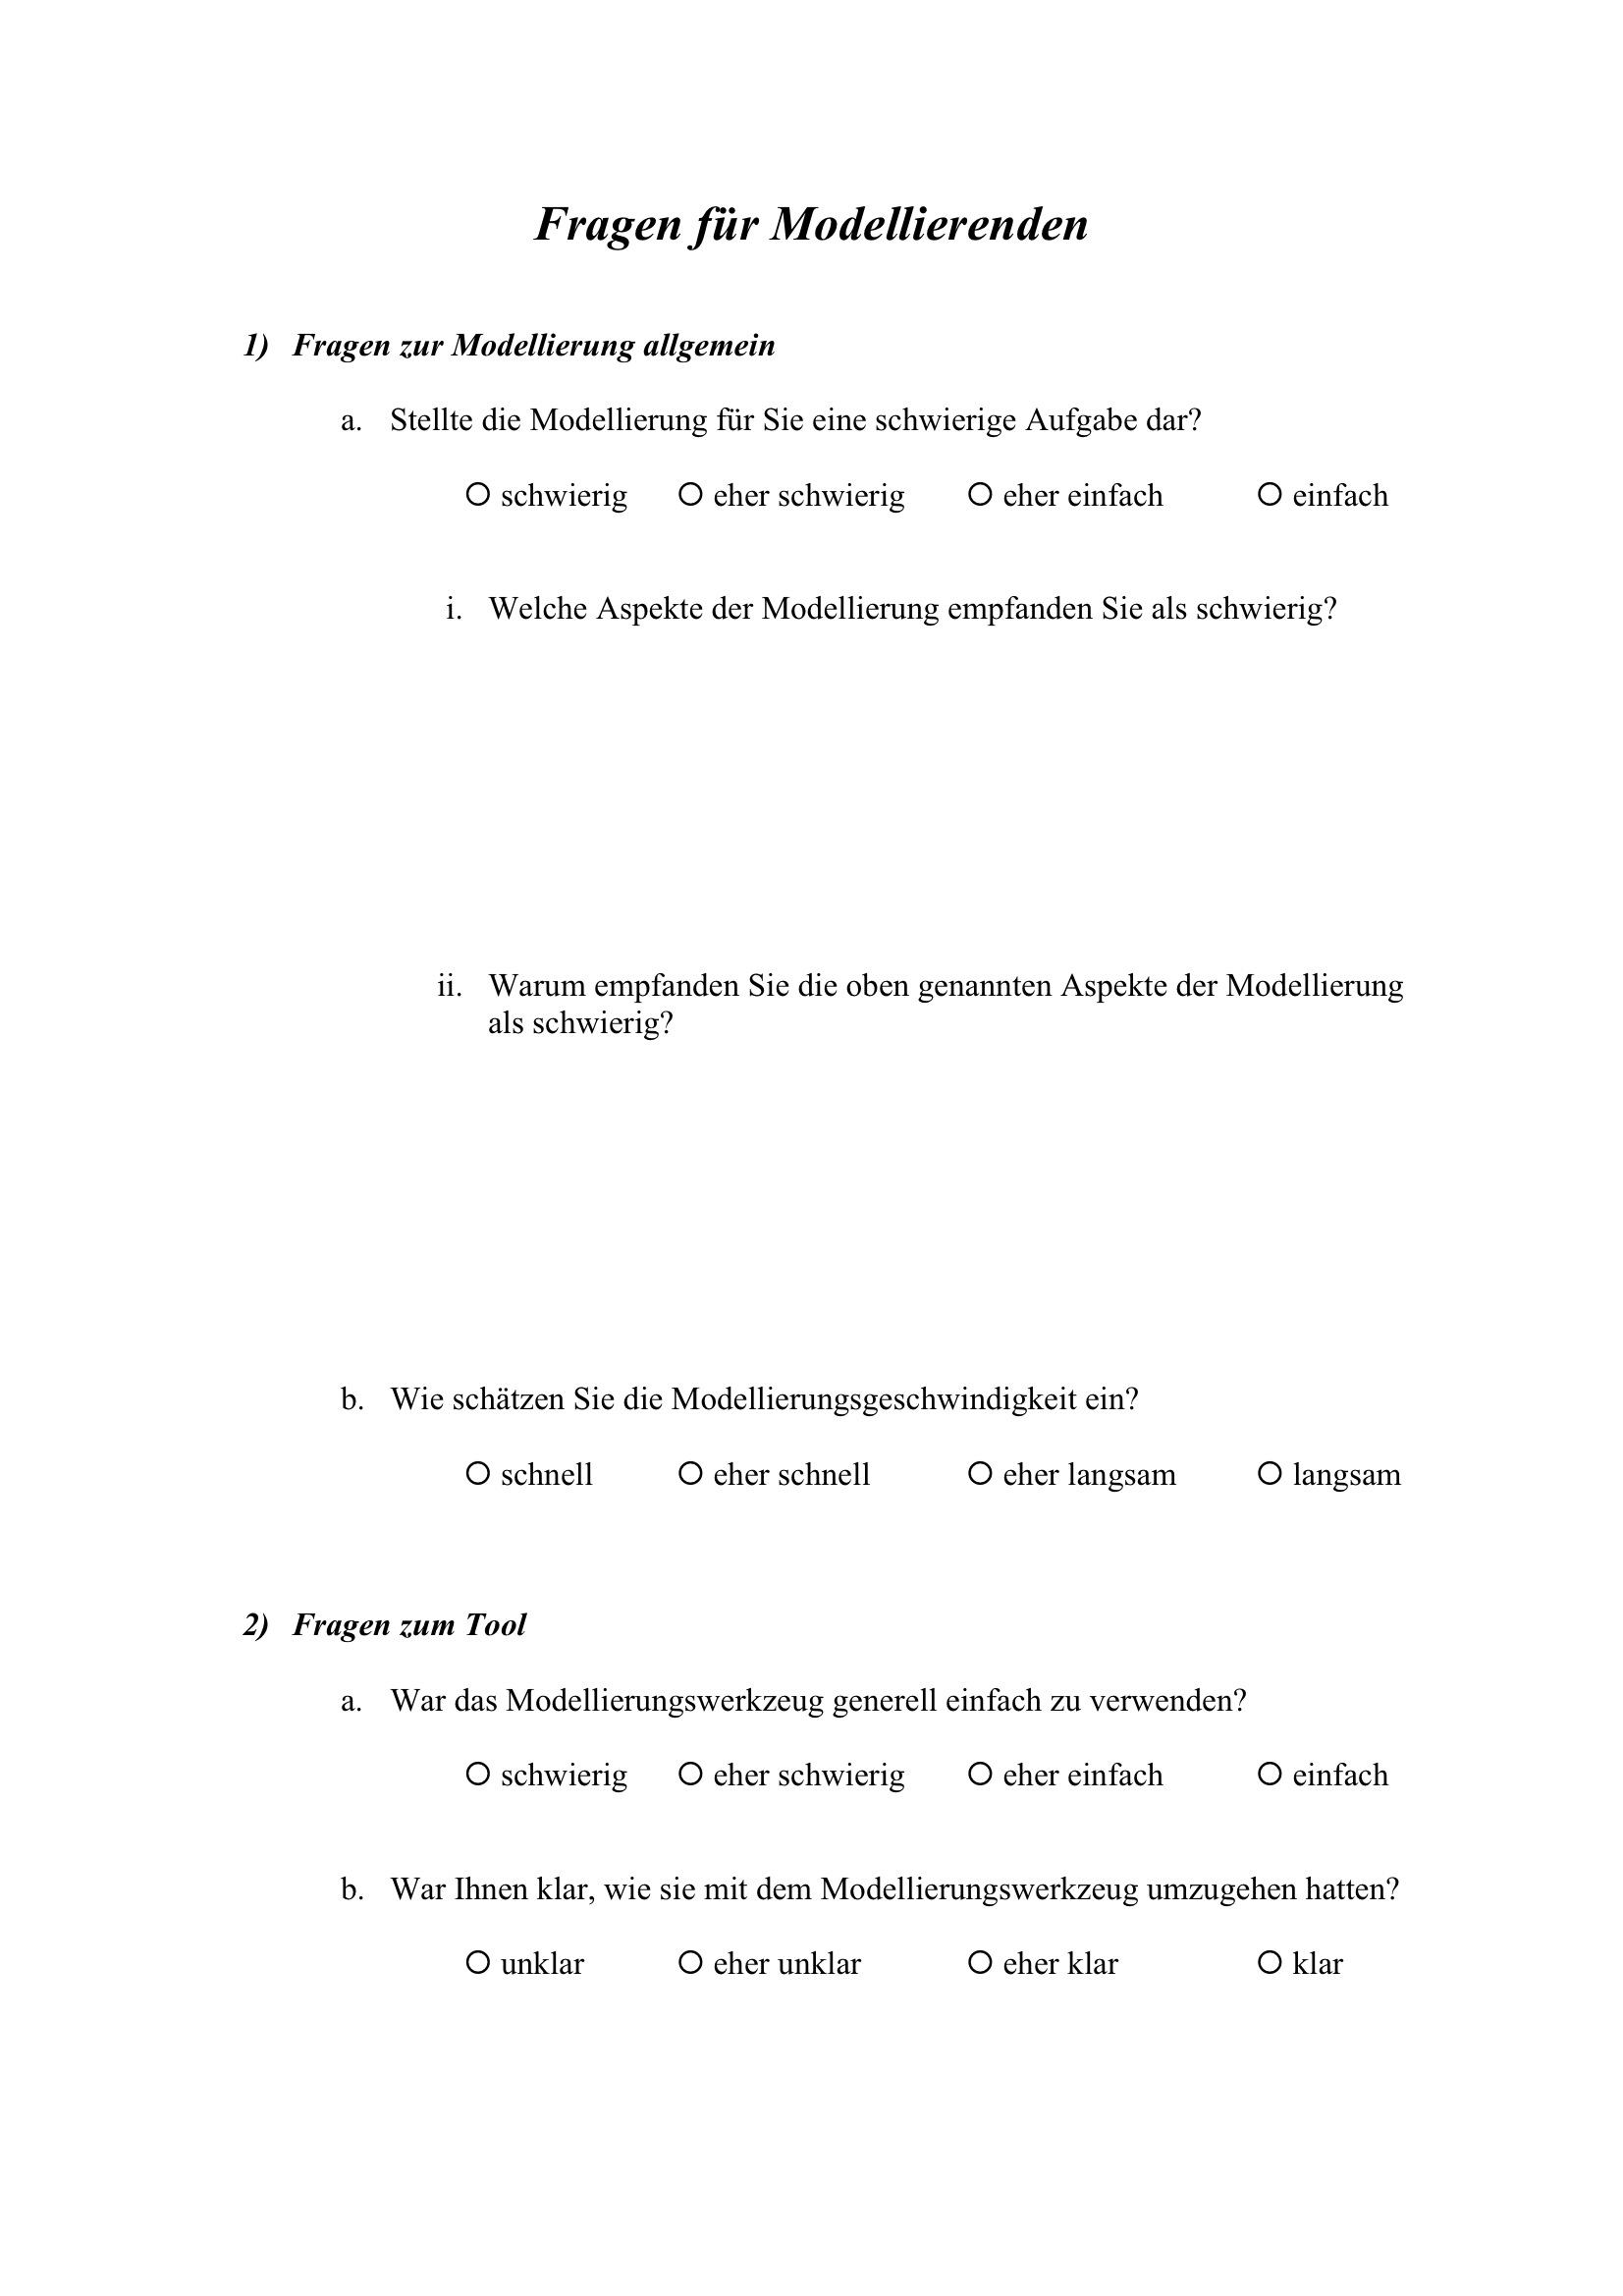
\includegraphics[width=0.9\textwidth]{img/AnhangEmpirie/fb1_1-01.jpeg}%
	}
	\caption{Erster Fragebogen für Modellierer in Evaluierungsblock 1 - Seite 1}
	\label{fig:img_AnhangEmpirie_fb1_1-01}
\end{figure}

\begin{figure}[htbp]
	\centering
	\fbox{%
		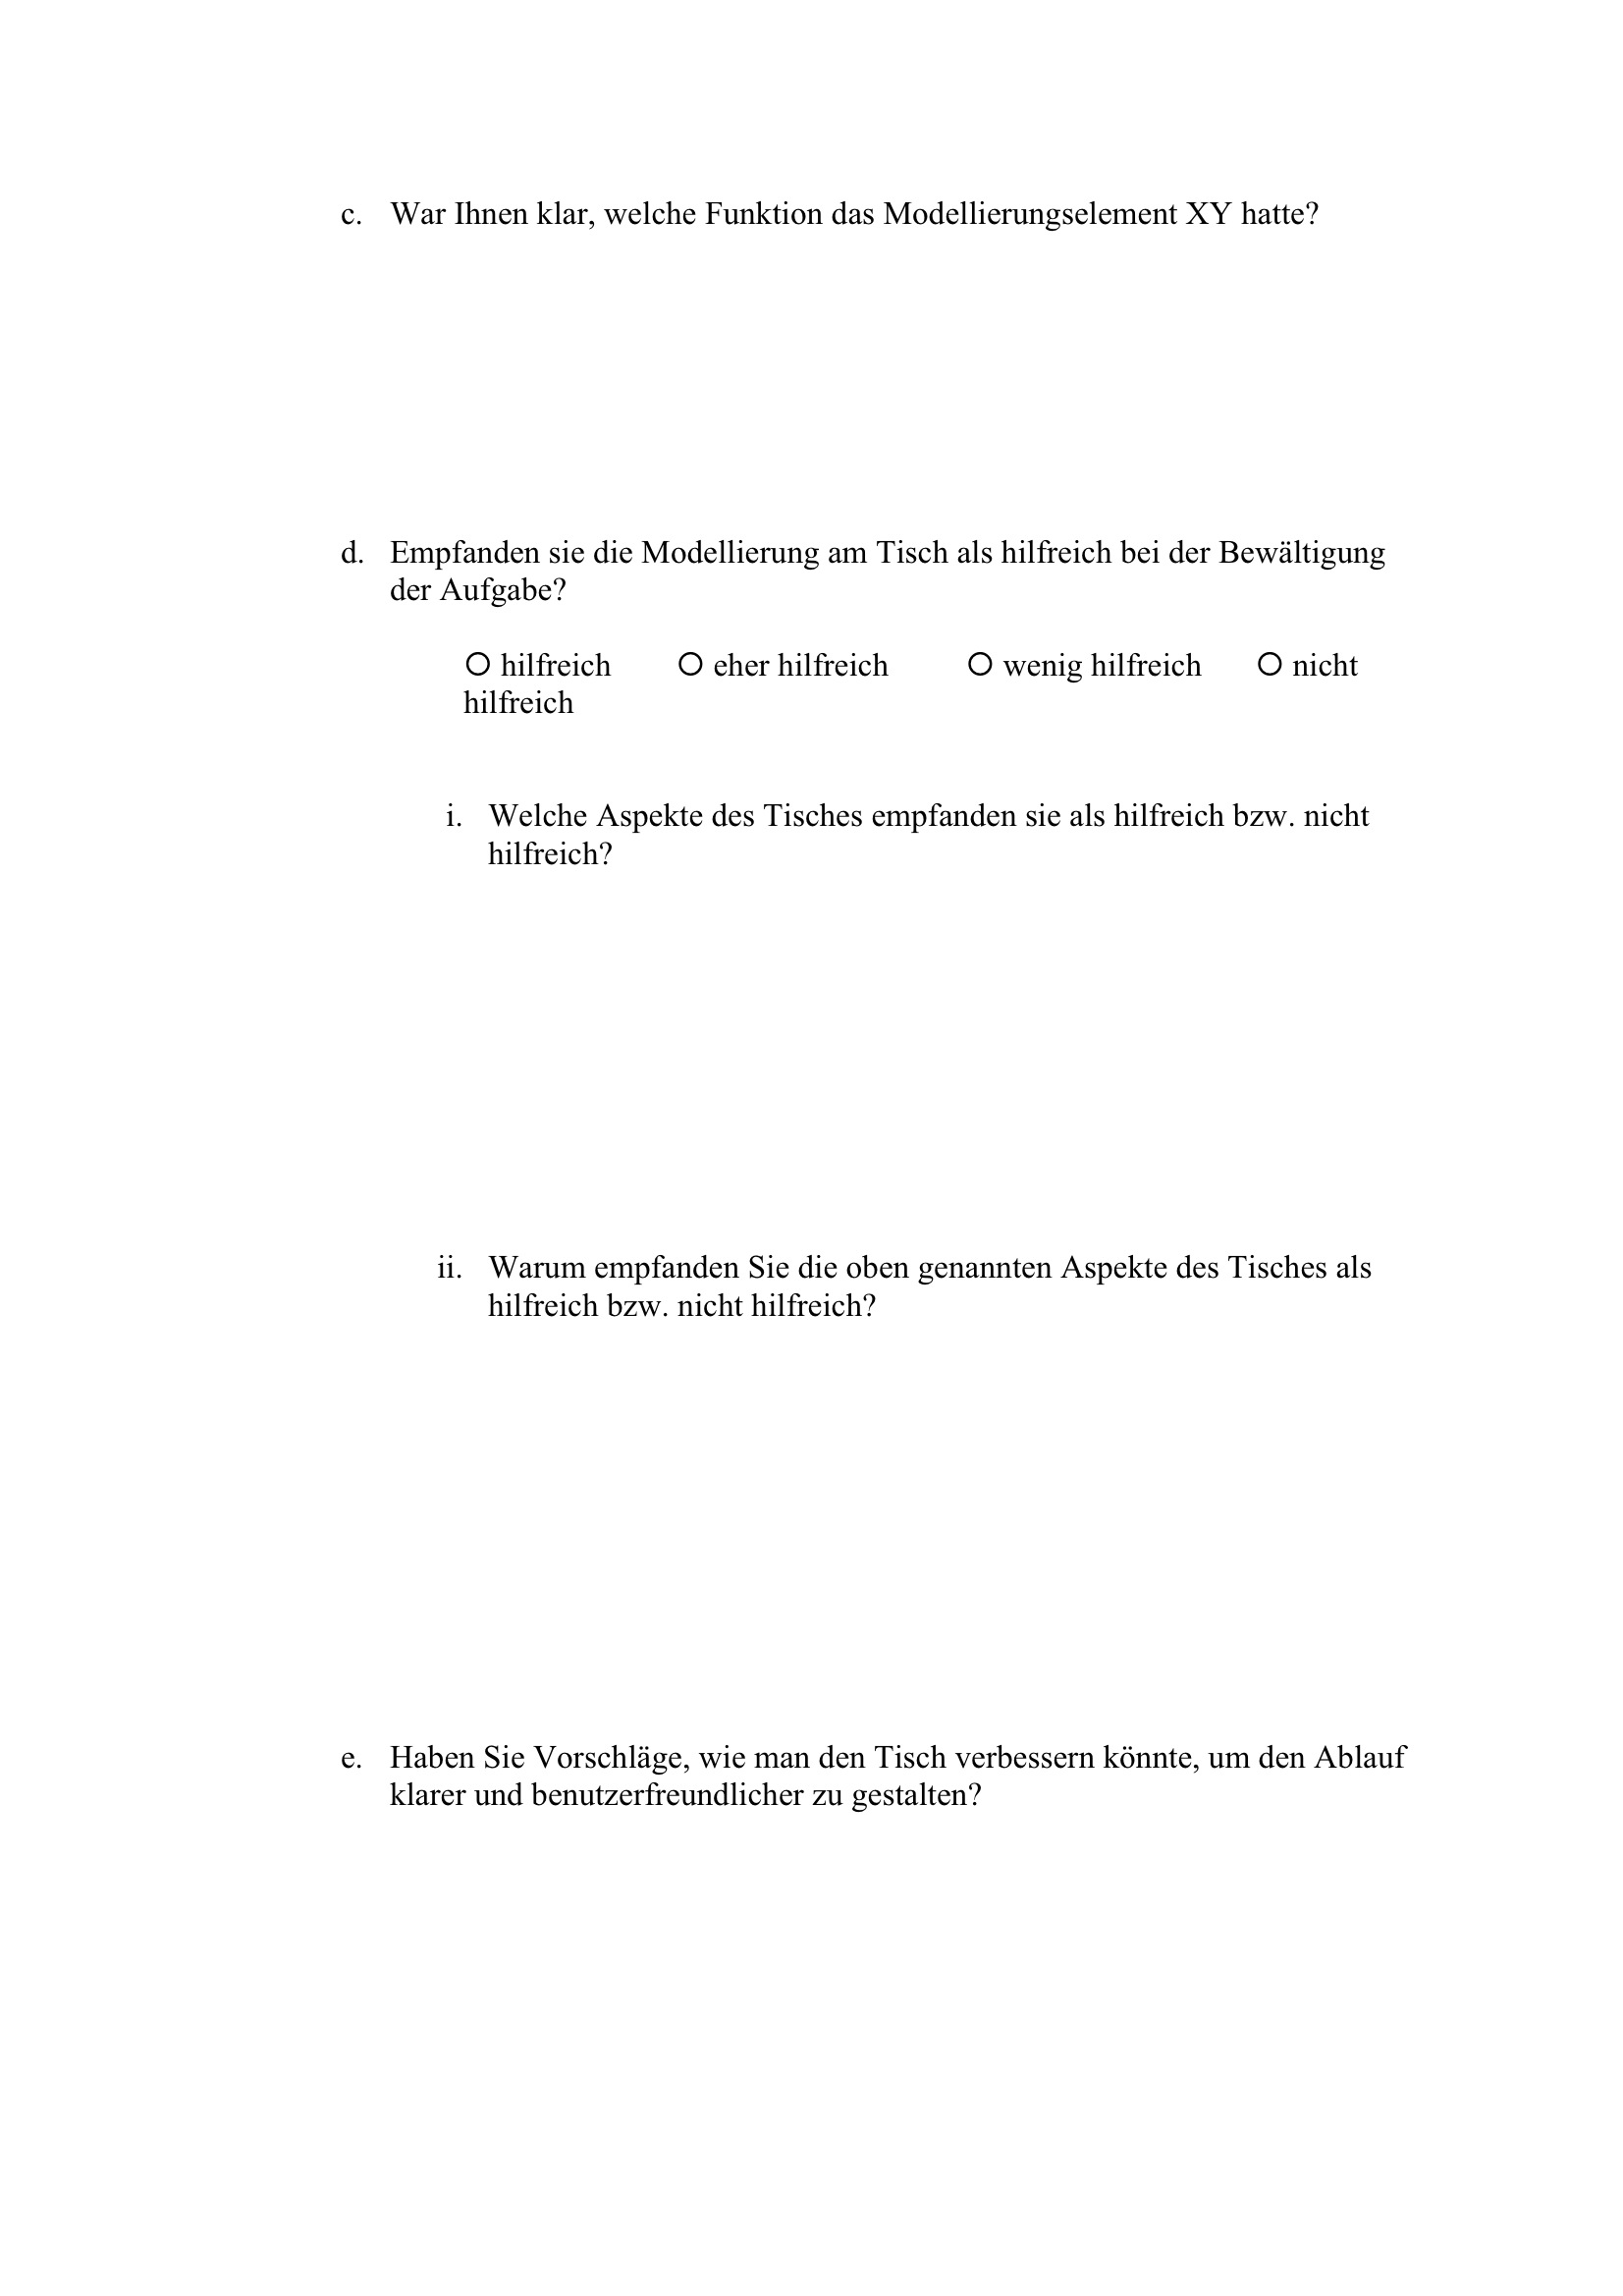
\includegraphics[width=0.9\textwidth]{img/AnhangEmpirie/fb1_1-02.jpeg}%
	}
	\caption{Erster Fragebogen für Modellierer in Evaluierungsblock 1 - Seite 2}
	\label{fig:img_AnhangEmpirie_fb1_1-02}
\end{figure}

\begin{figure}[htbp]
	\centering
	\fbox{%
		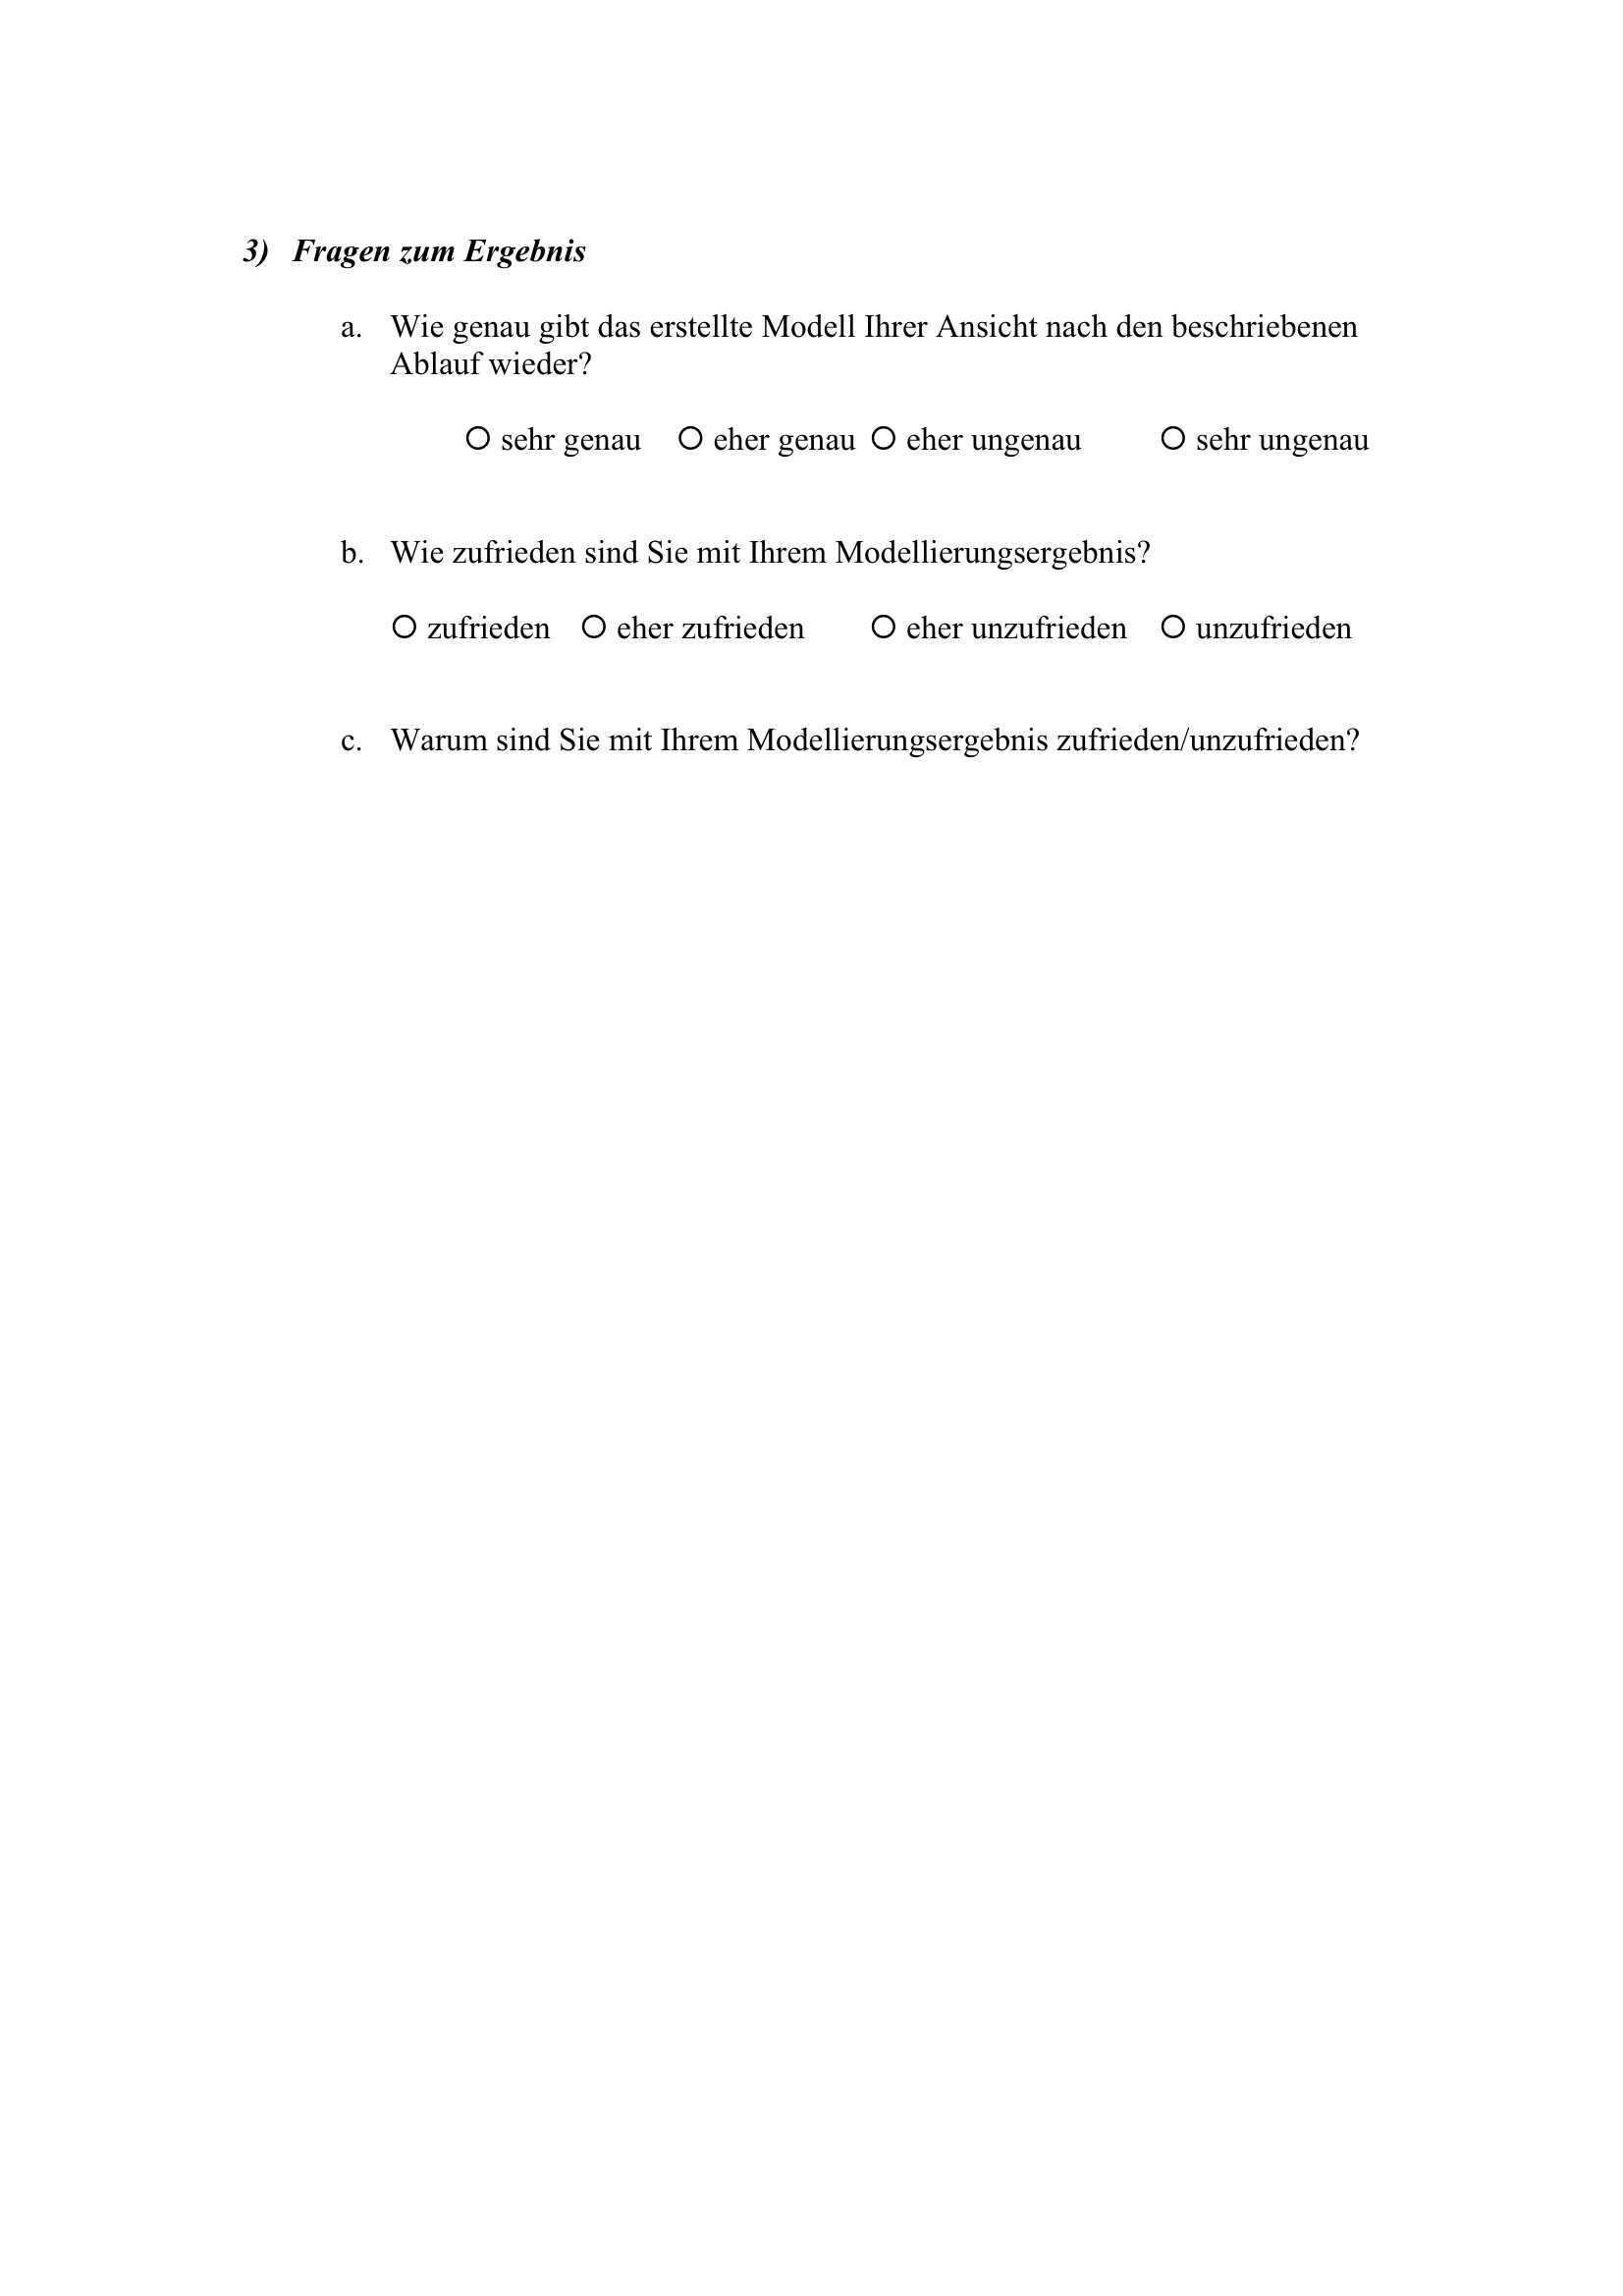
\includegraphics[width=0.9\textwidth]{img/AnhangEmpirie/fb1_1-03.jpeg}%
	}
	\caption{Erster Fragebogen für Modellierer in Evaluierungsblock 1 - Seite 3}
	\label{fig:img_AnhangEmpirie_fb1_1-03}
\end{figure}

\begin{figure}[htbp]
	\centering
	\fbox{%
		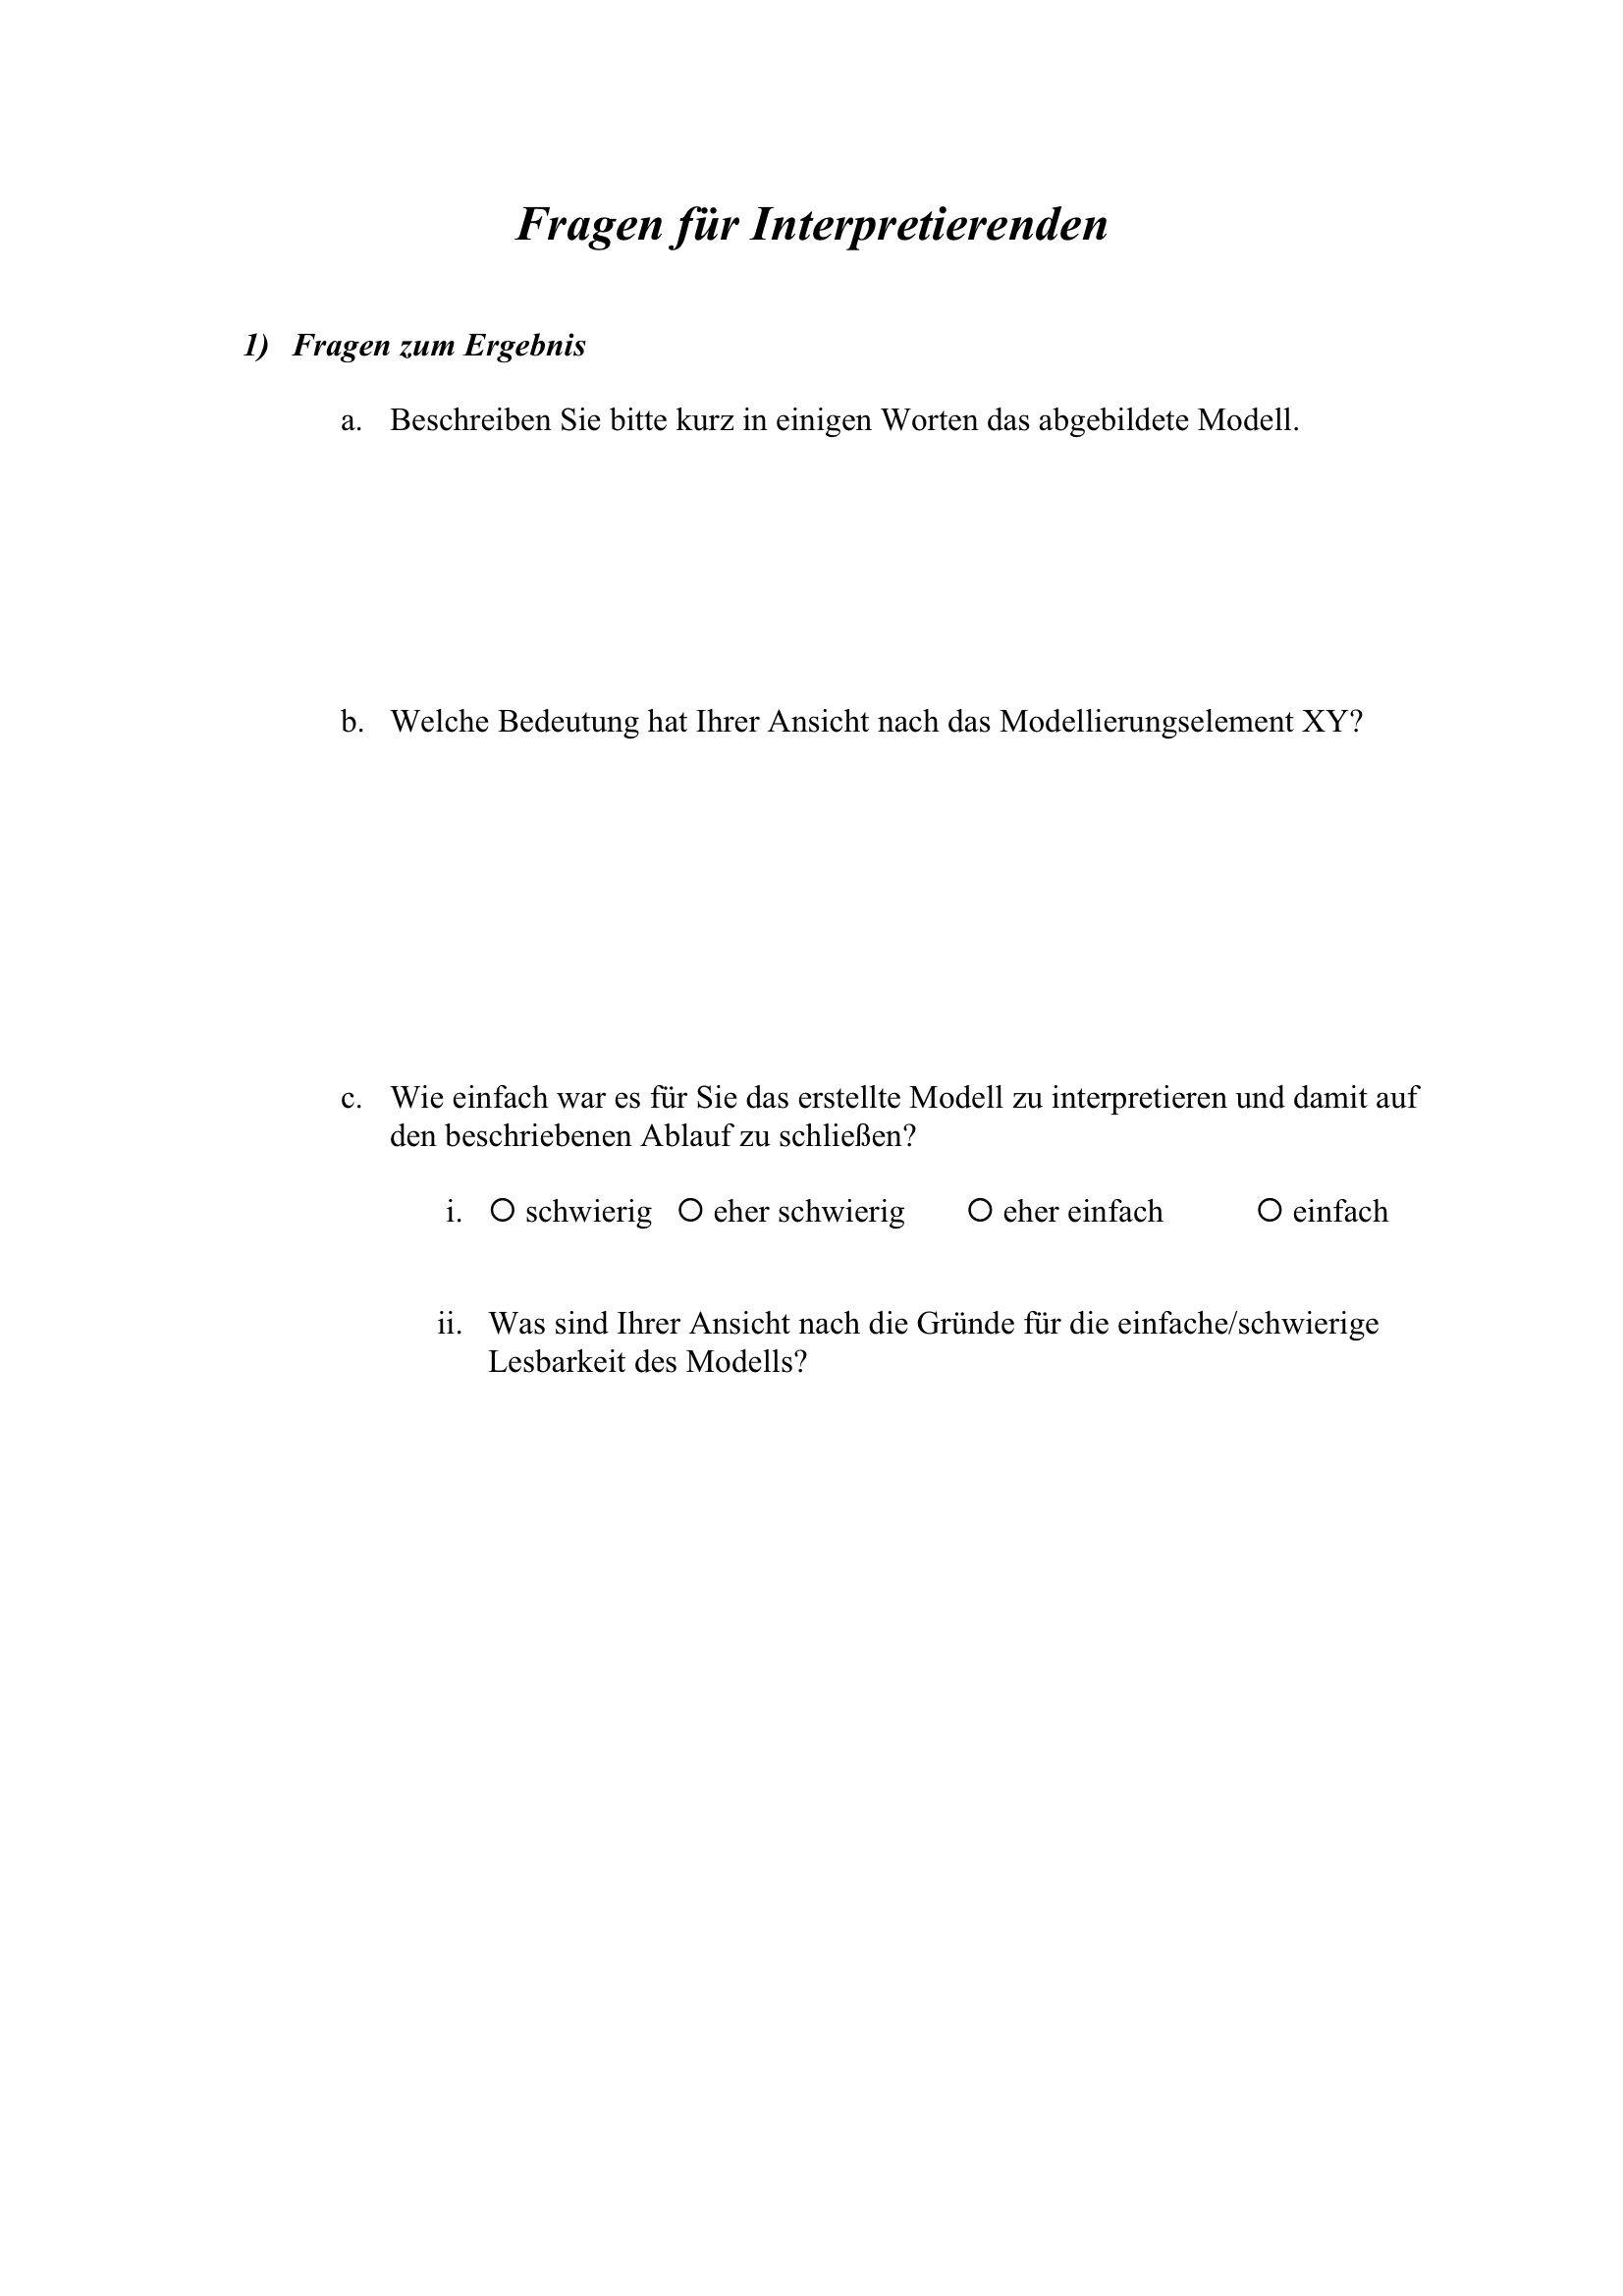
\includegraphics[width=0.9\textwidth]{img/AnhangEmpirie/fb1_2-01.jpeg}%
	}
	\caption{Fragebogen für Interpretierer in Evaluierungsblock 1 - Seite 1}
	\label{fig:img_AnhangEmpirie_fb1_2-01}
\end{figure}

\begin{figure}[htbp]
	\centering
	\fbox{%
		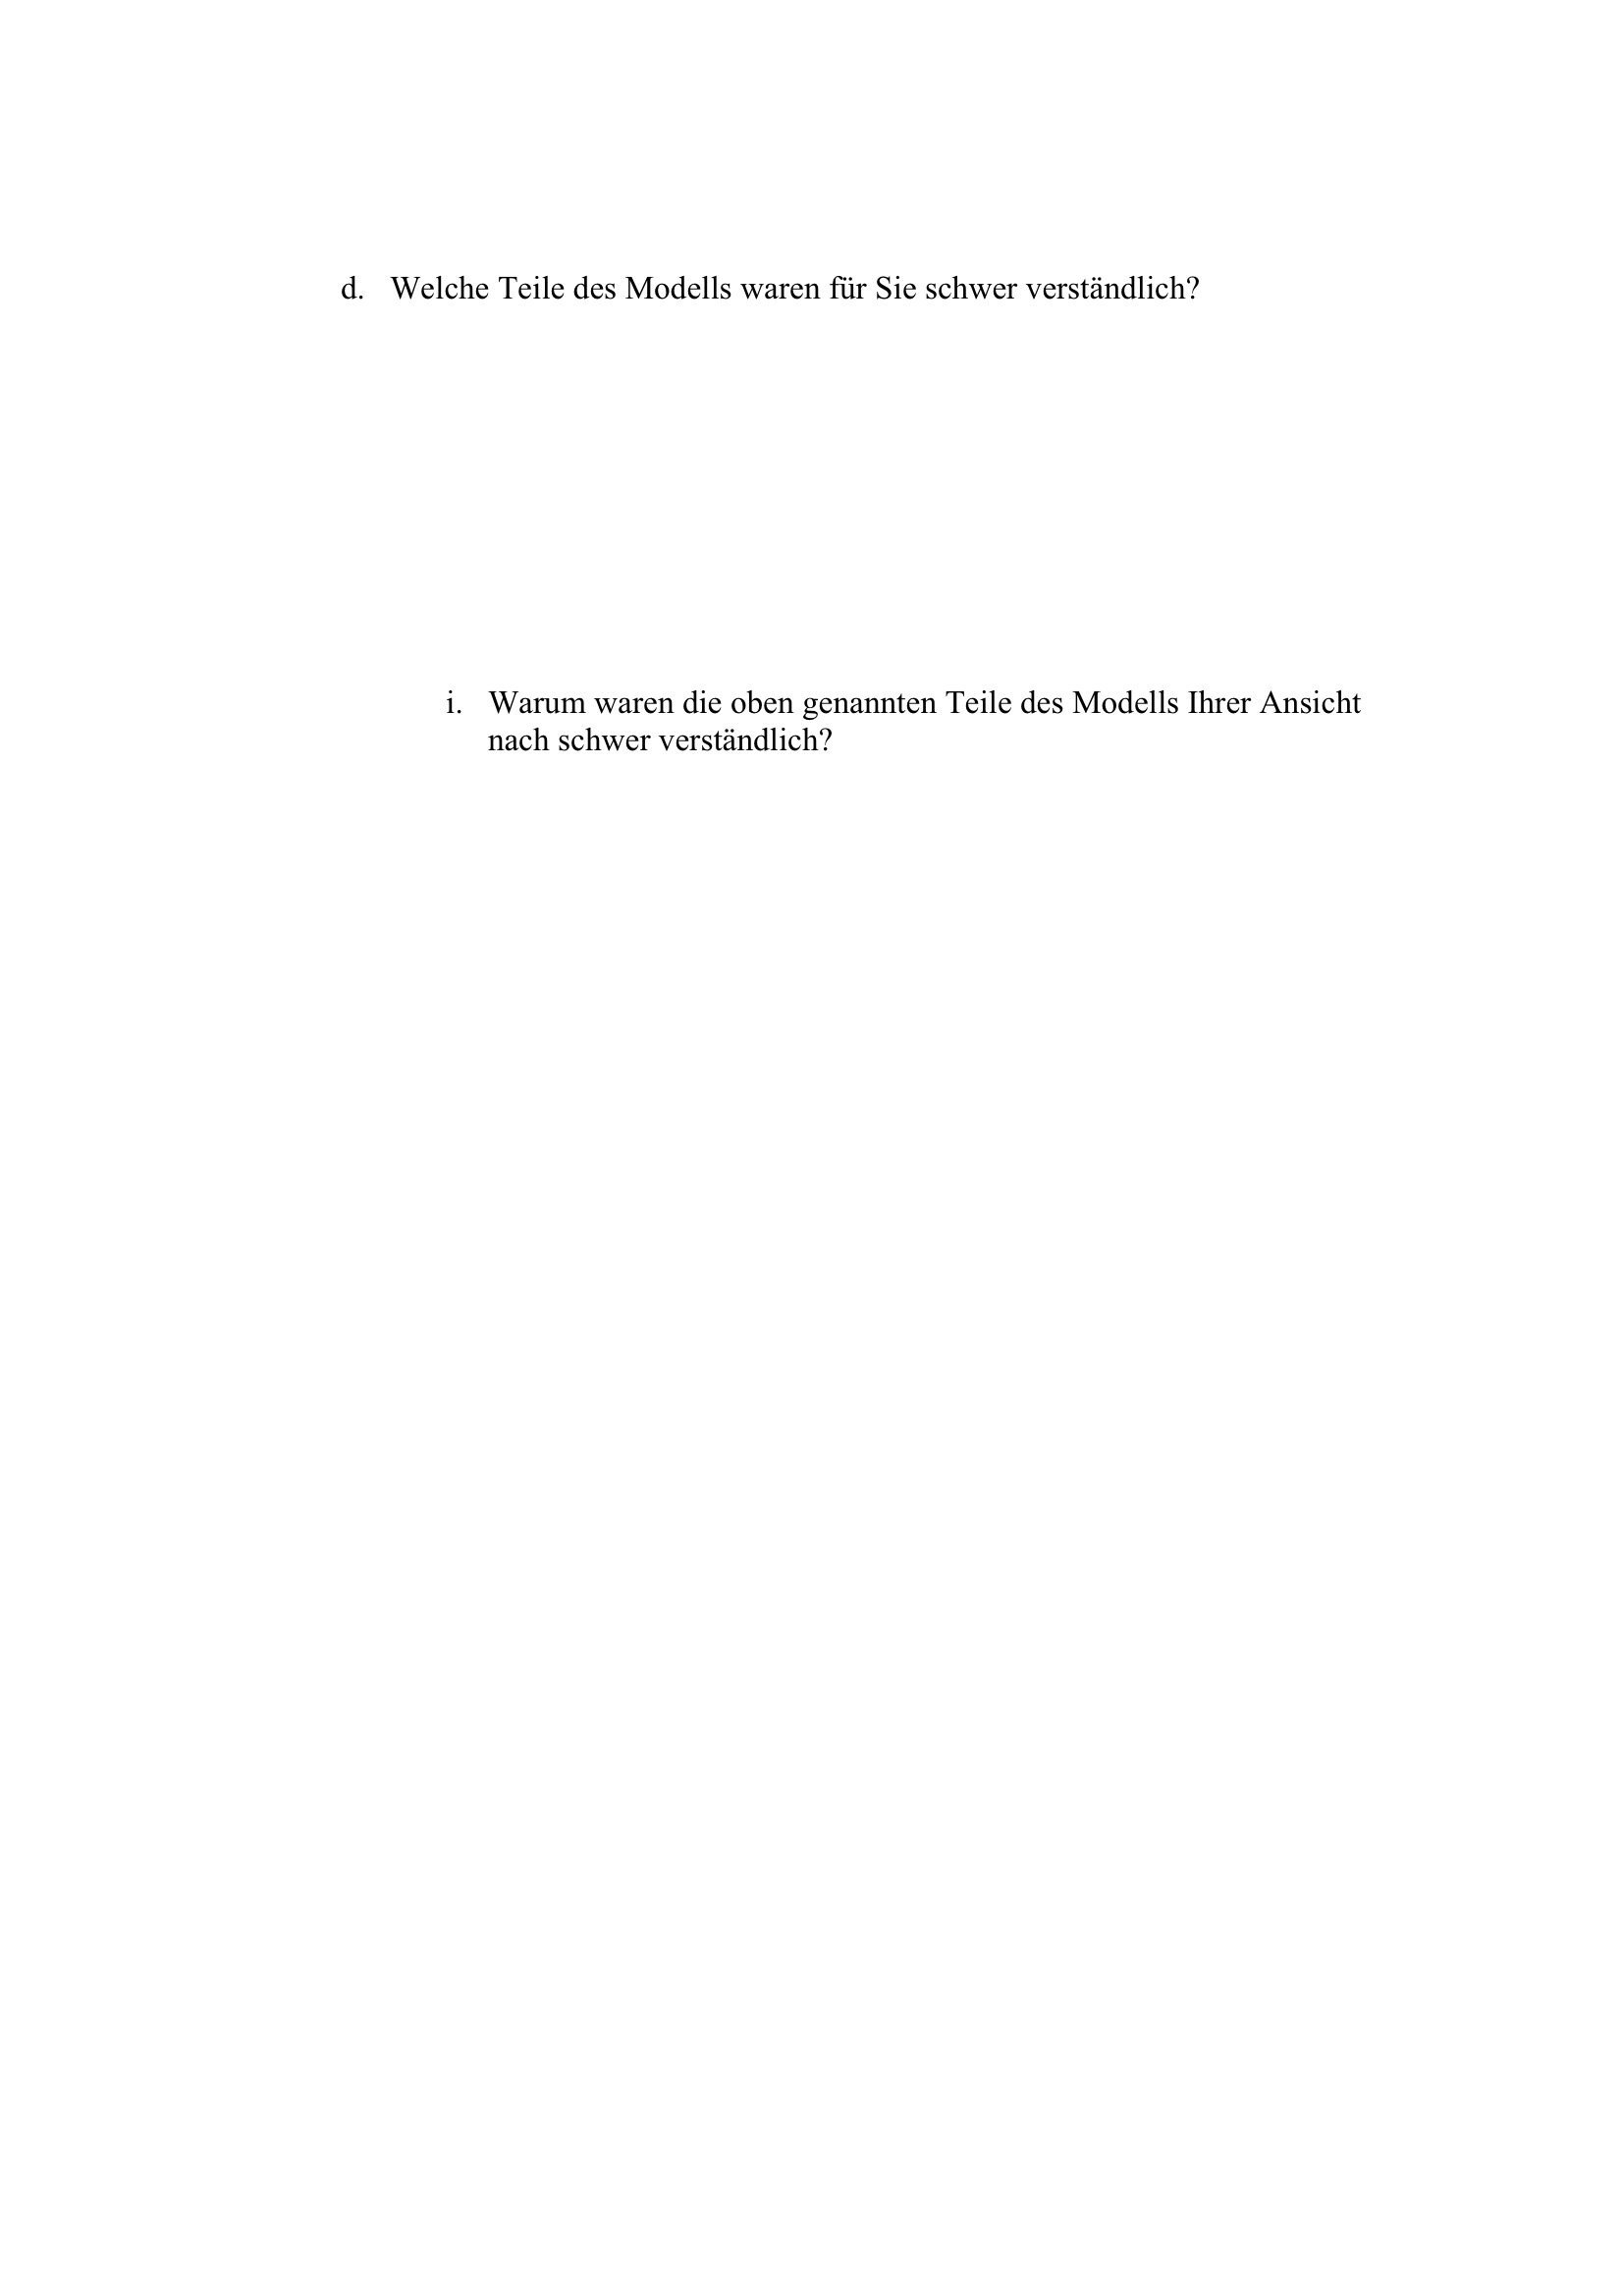
\includegraphics[width=0.9\textwidth]{img/AnhangEmpirie/fb1_2-02.jpeg}%
	}
	\caption{Fragebogen für Interpretierer in Evaluierungsblock 1 - Seite 2}
	\label{fig:img_AnhangEmpirie_fb1_2-02}
\end{figure}

\begin{figure}[htbp]
	\centering
	\fbox{%
		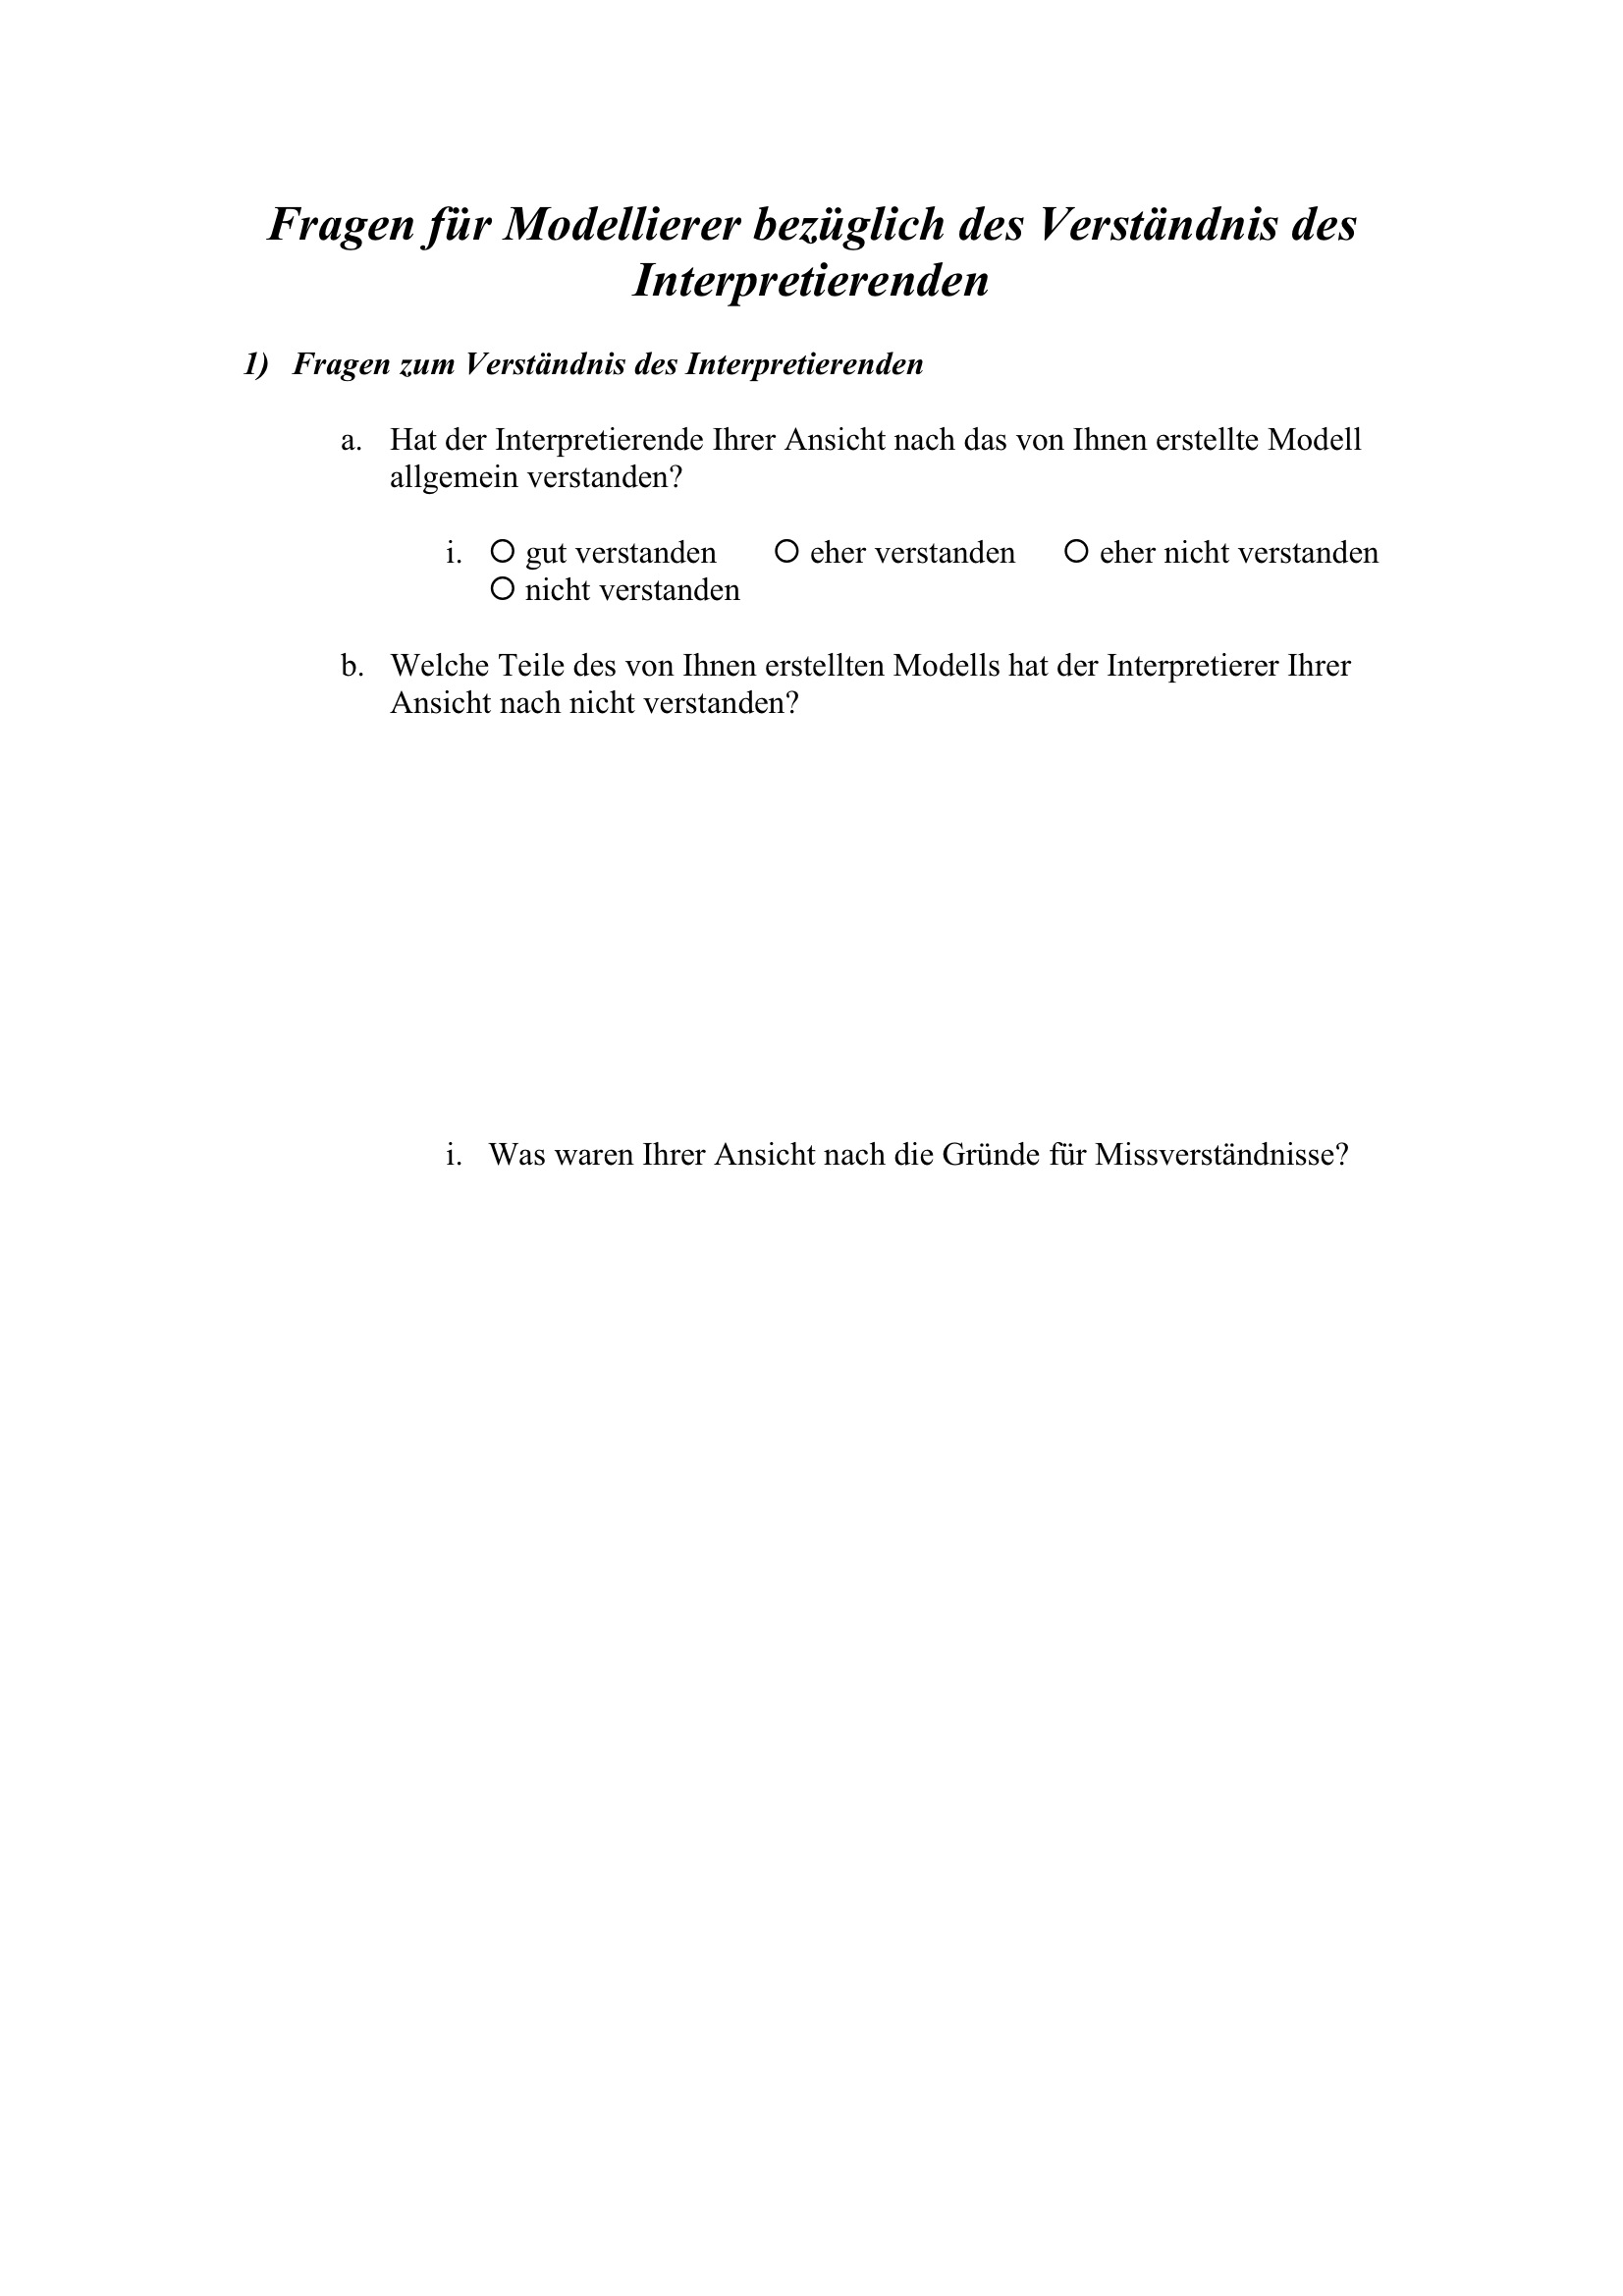
\includegraphics[width=0.9\textwidth]{img/AnhangEmpirie/fb1_3-01.jpeg}%
	}
	\caption{Fragebogen bezüglich der Korrektheit der Interpretation in Evaluierungsblock 1}
	\label{fig:img_AnhangEmpirie_fb1_3-01}
\end{figure}

\begin{figure}[htbp]
	\centering
	\fbox{%
		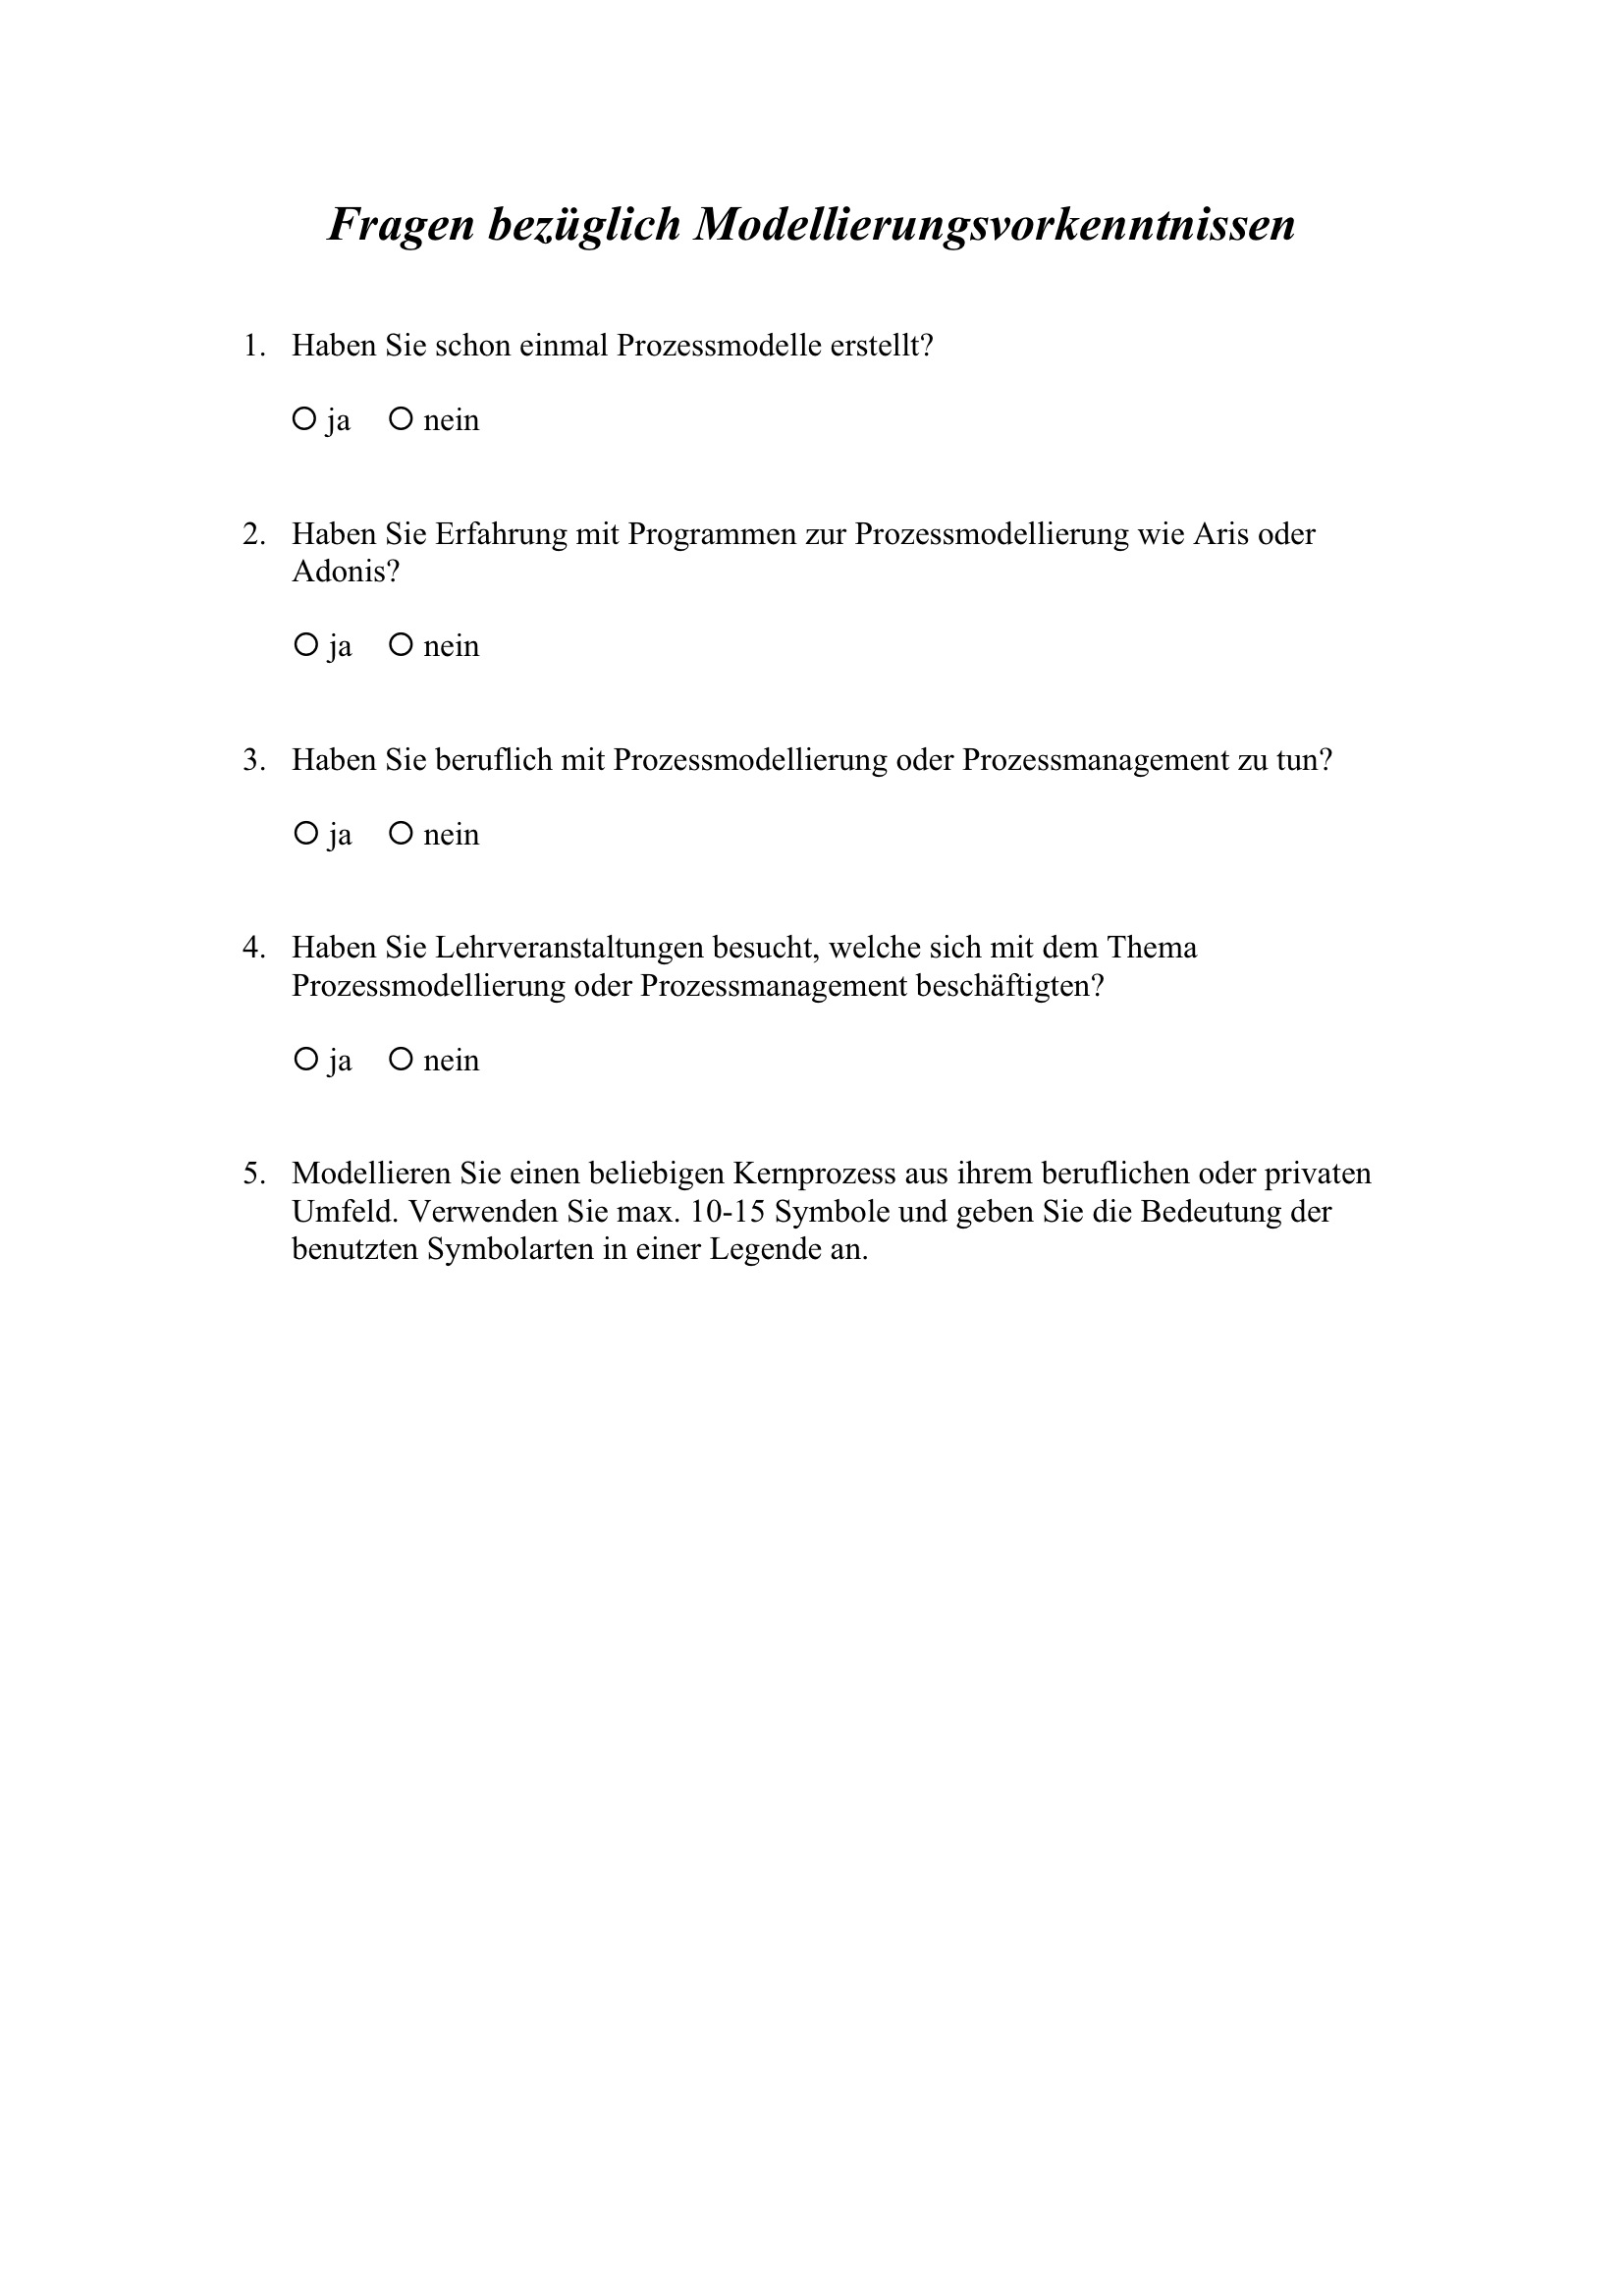
\includegraphics[width=0.9\textwidth]{img/AnhangEmpirie/fb1_4-01.jpeg}%
	}
	\caption{Fragebogen bezüglich Modellierungsvorkenntnissen in Evaluierungsblock 1}
	\label{fig:img_AnhangEmpirie_fb1_4-01}
\end{figure}

\clearpage
\subsection{Fragebögen aus Evaluierungsblock 4}
\label{sub:fb_eval4}

Die Abbildungen \ref{fig:img_AnhangEmpirie_fb4_1-01} bis \ref{fig:img_AnhangEmpirie_fb4_1-08} zeigen den ersten in Evaluierungsblock 4 verwendeten Fragebogen. Die Abbildungen \ref{fig:img_AnhangEmpirie_fb4_2-01} bis \ref{fig:img_AnhangEmpirie_fb4_2-08} zeigen den zweiten in Evaluierungsblock 4 verwendeten Fragebogen. Der Aufbau der Fragebögen wurde von \citet{Wahlmuller10} detailliert beschrieben und begründet.

\begin{figure}[htbp]
	\centering
	\fbox{%
		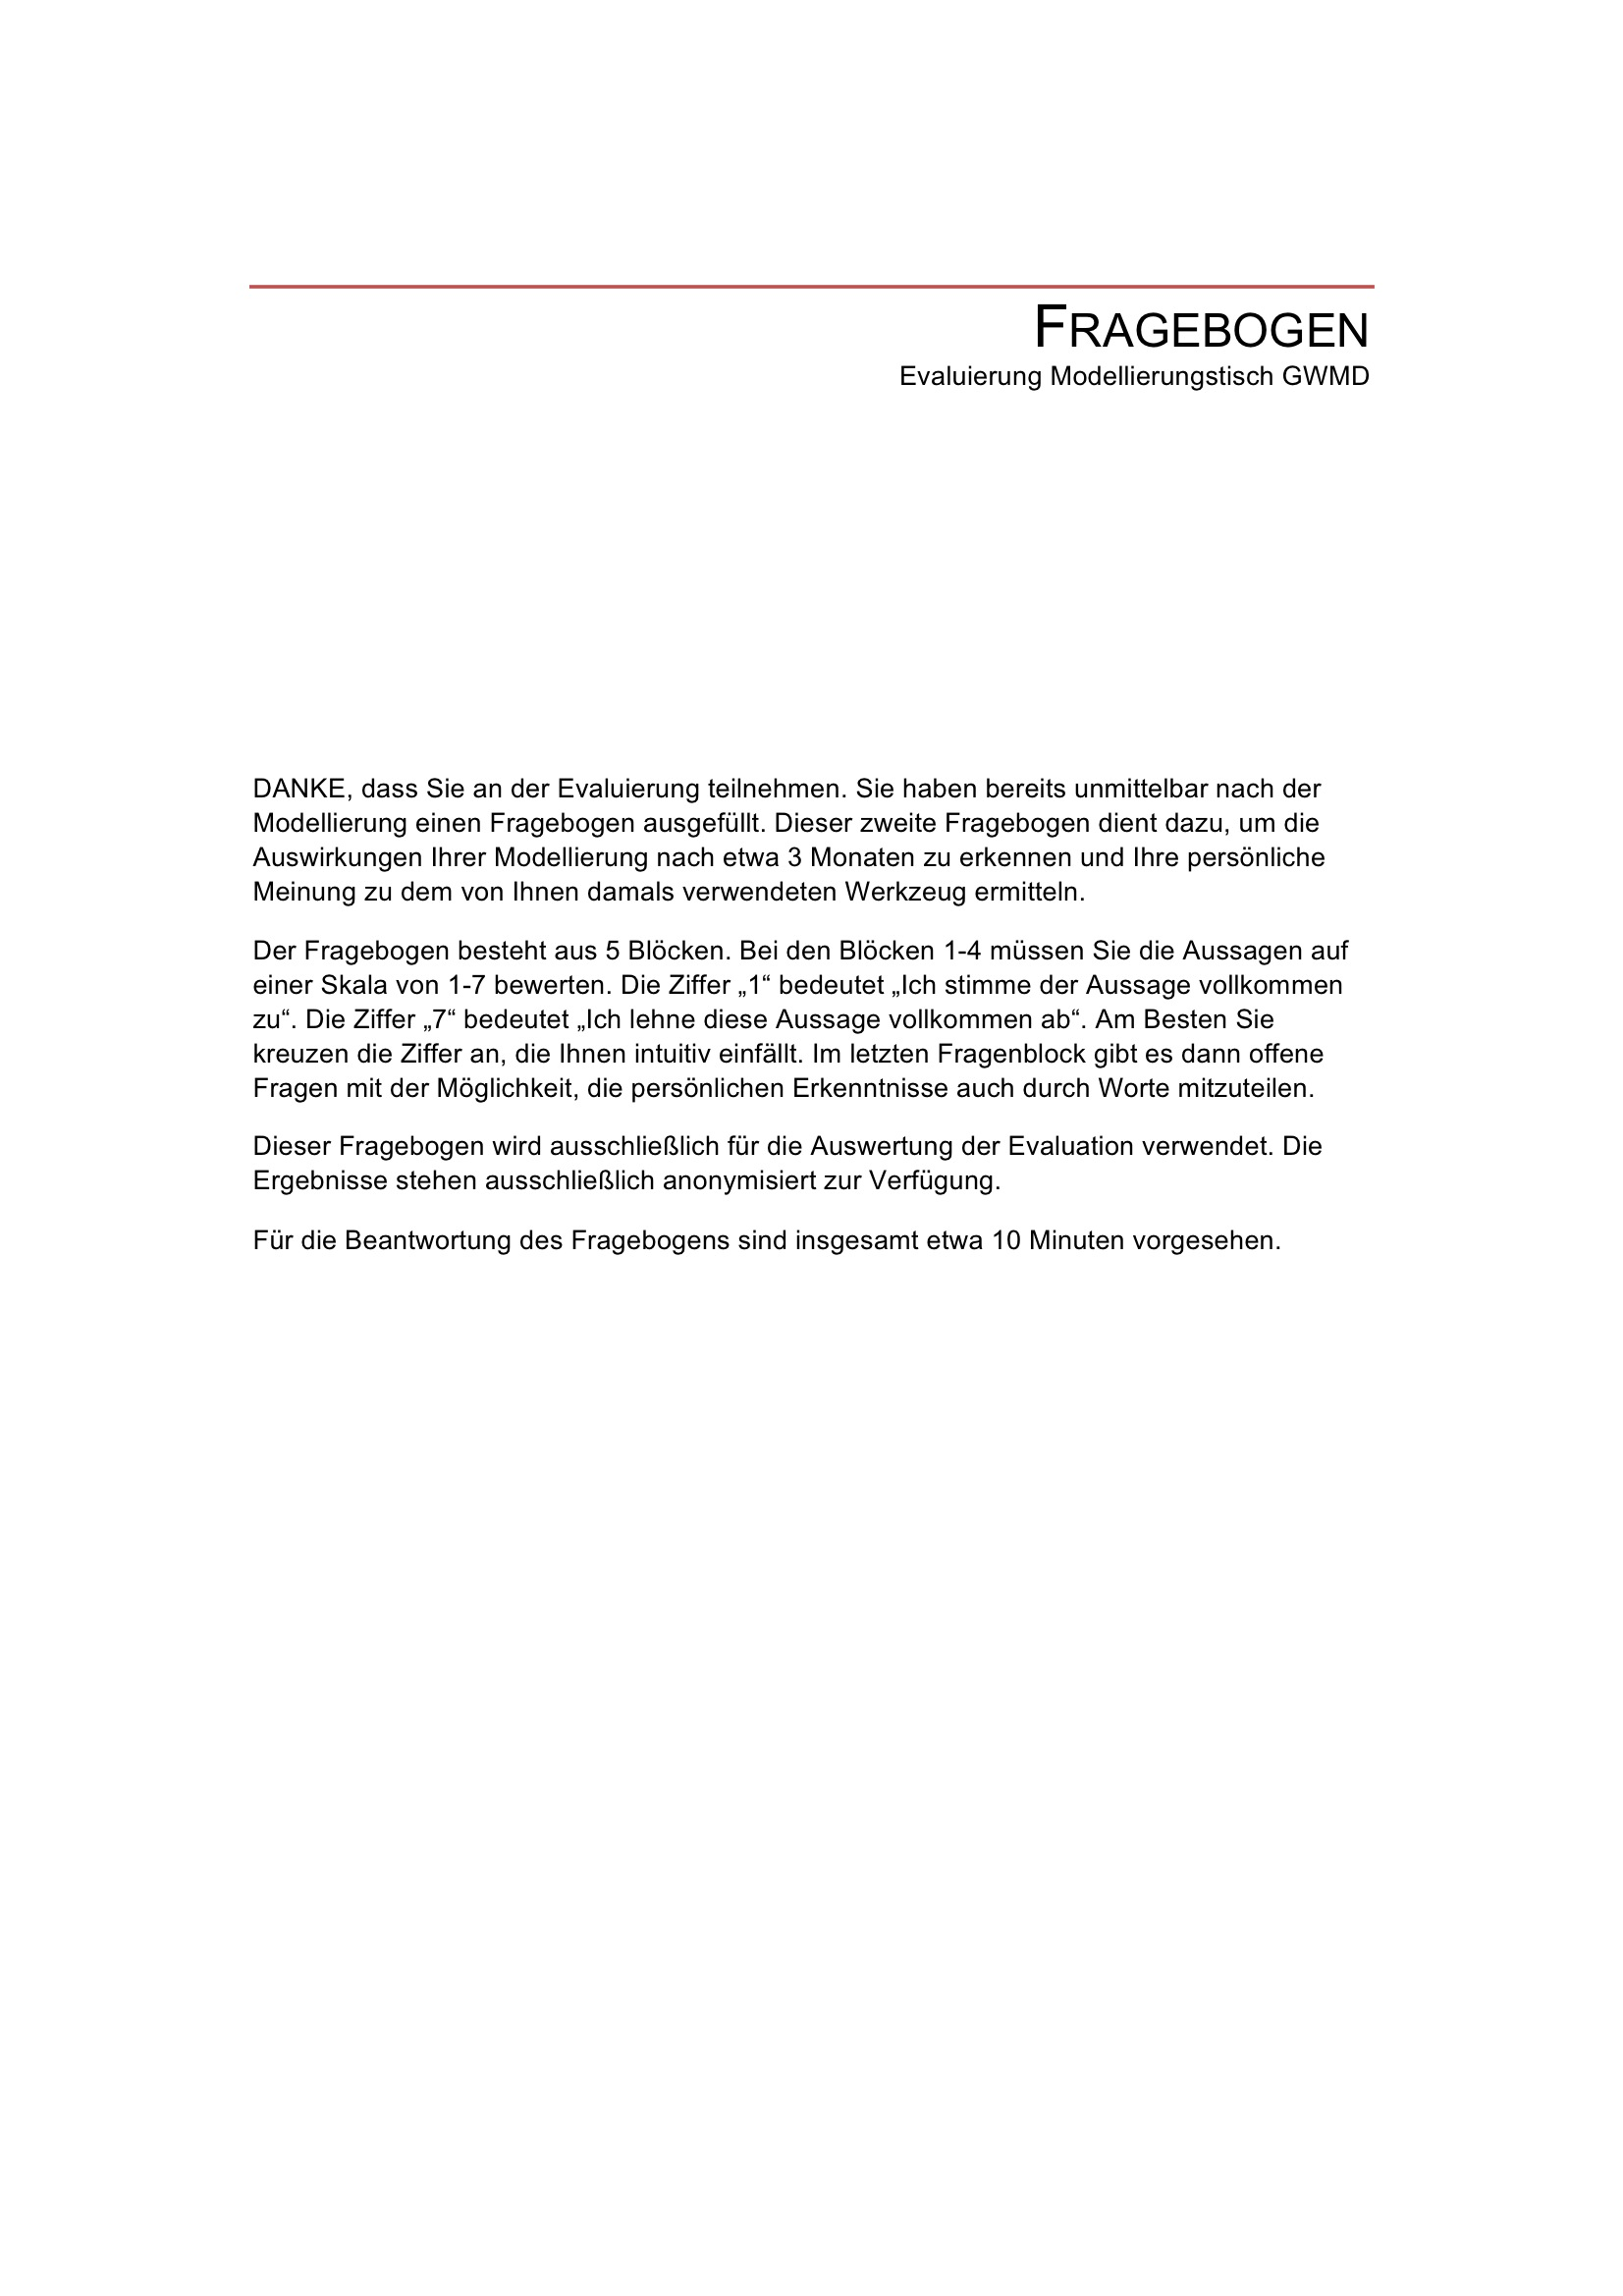
\includegraphics[width=0.9\textwidth]{img/AnhangEmpirie/fb4_1-01.jpeg}%
	}
	\caption{Erster Fragebogen für Evaluierungsblock 4 - Seite 1}
	\label{fig:img_AnhangEmpirie_fb4_1-01}
\end{figure}

\begin{figure}[htbp]
	\centering
	\fbox{%
		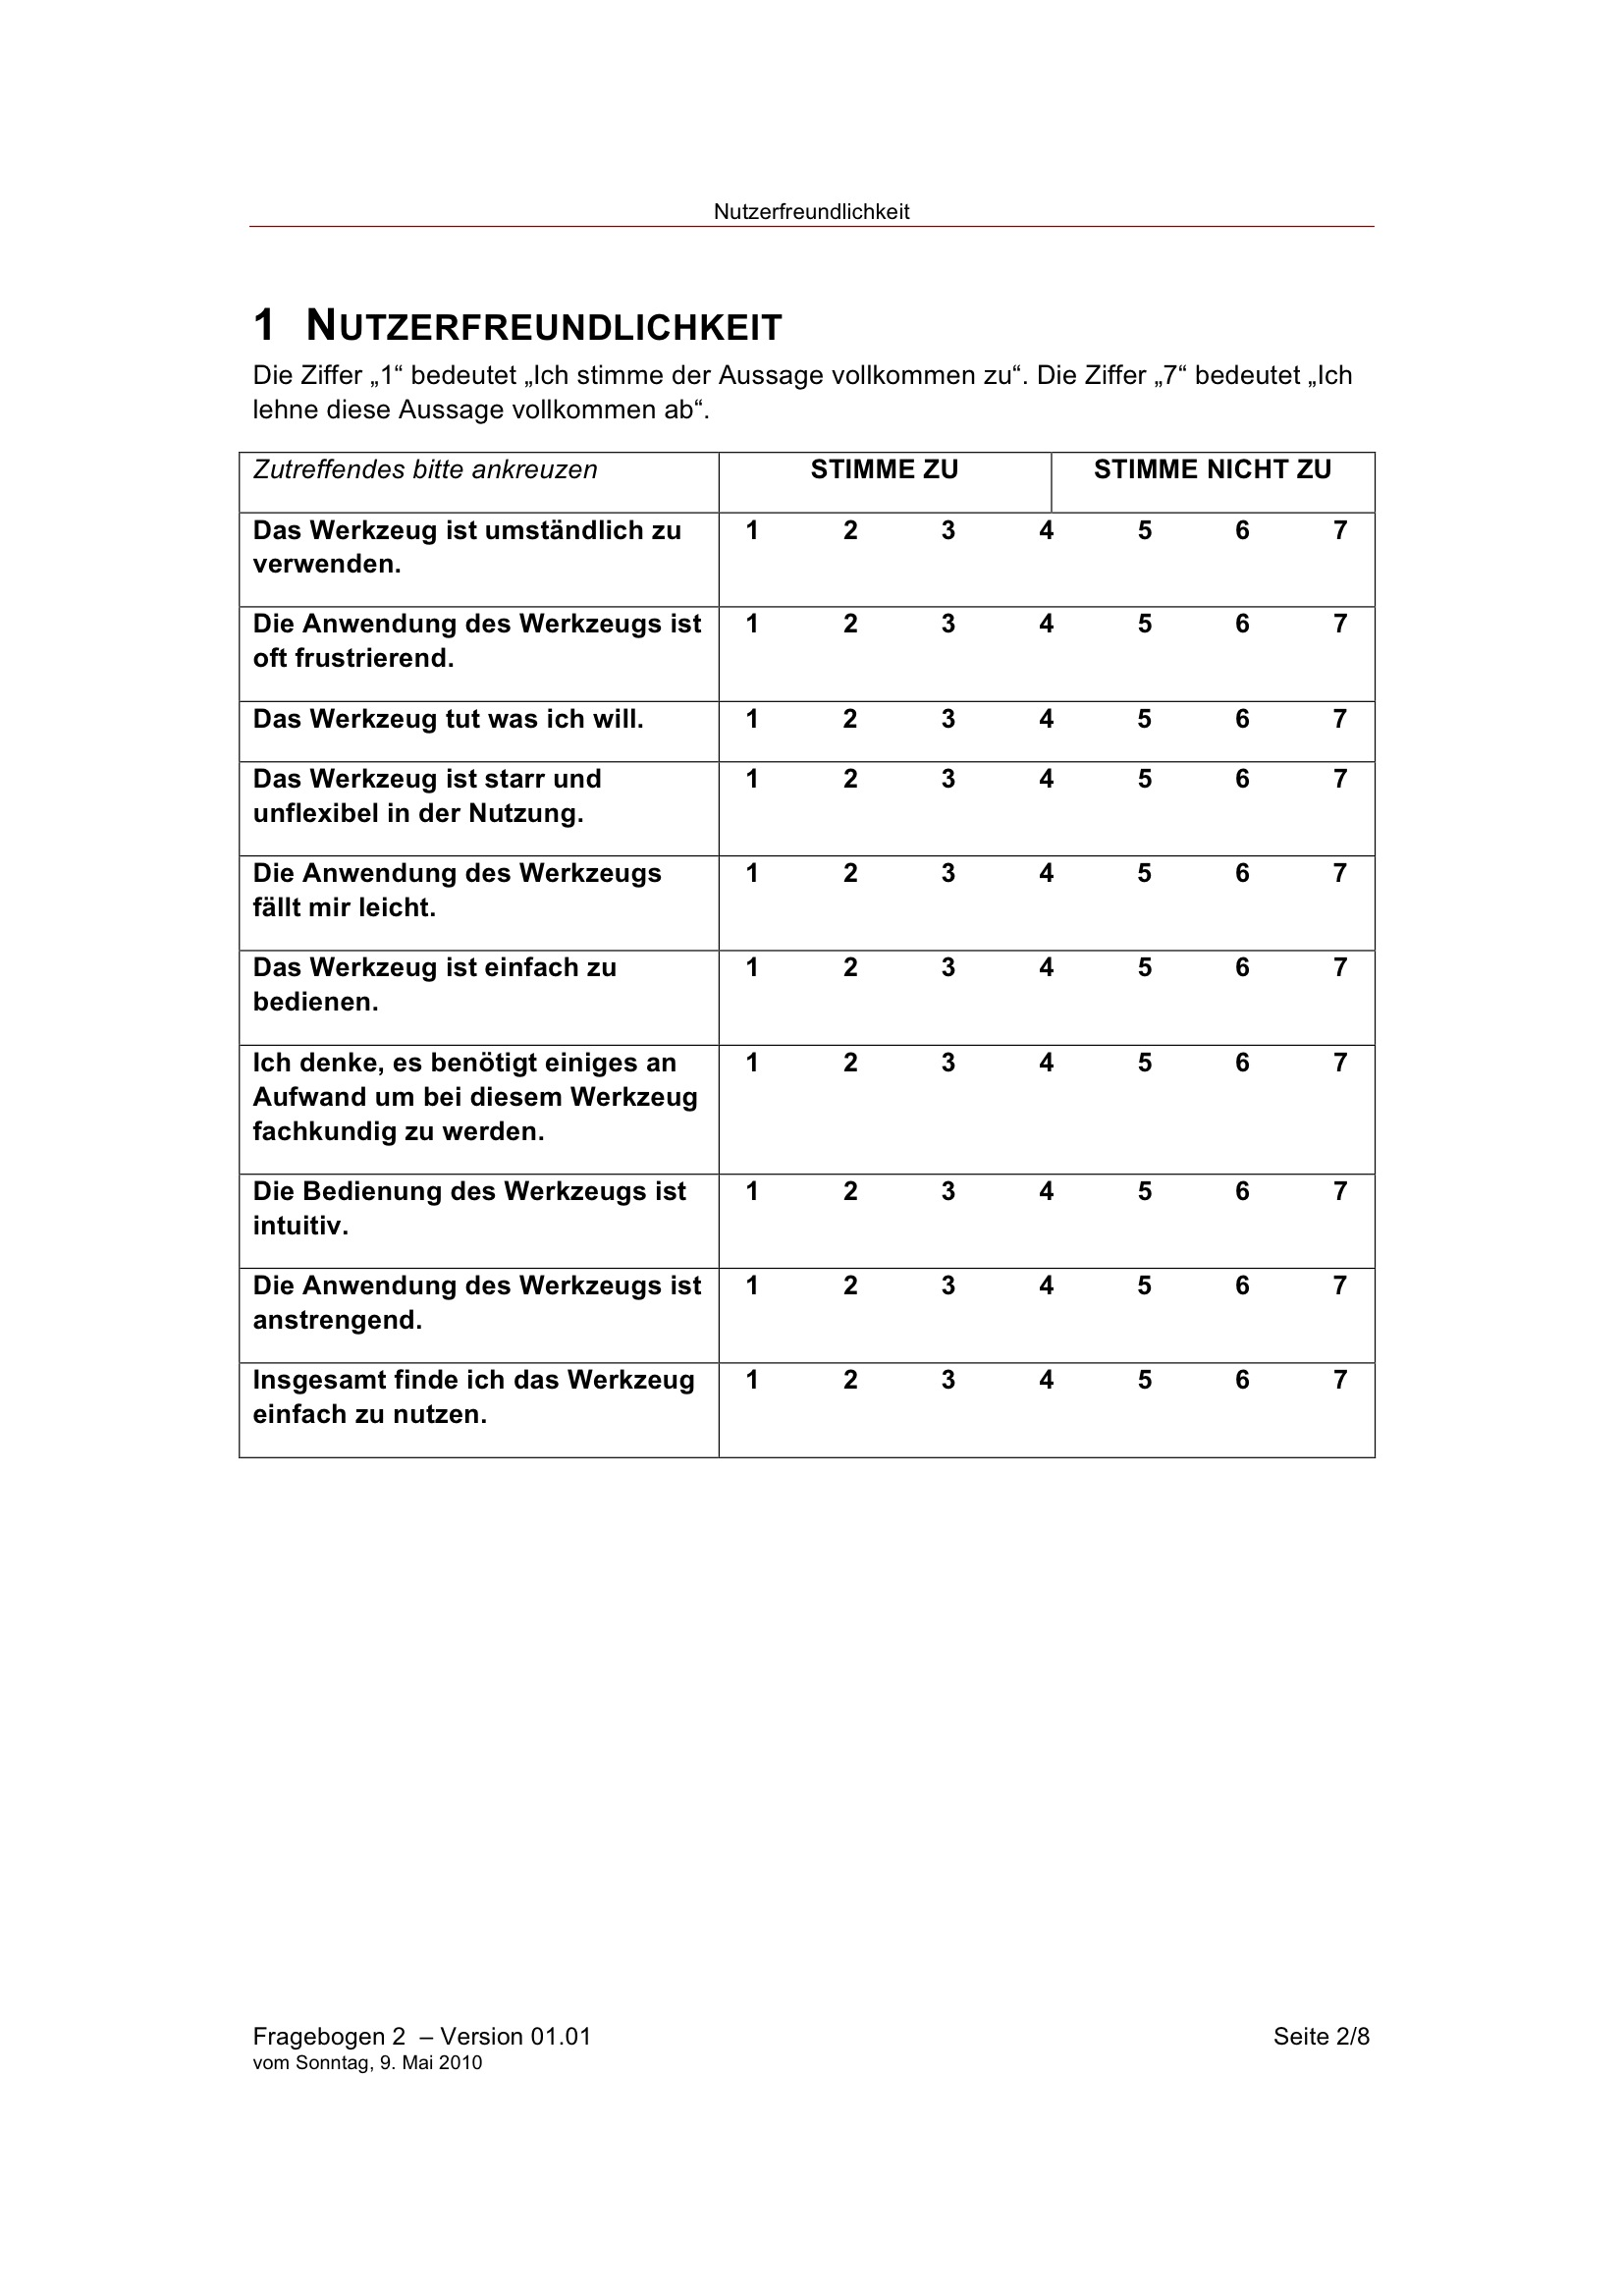
\includegraphics[width=0.9\textwidth]{img/AnhangEmpirie/fb4_1-02.jpeg}%
	}
	\caption{Erster Fragebogen für Evaluierungsblock 4 - Seite 2}
	\label{fig:img_AnhangEmpirie_fb4_1-02}
\end{figure}

\begin{figure}[htbp]
	\centering
	\fbox{%
		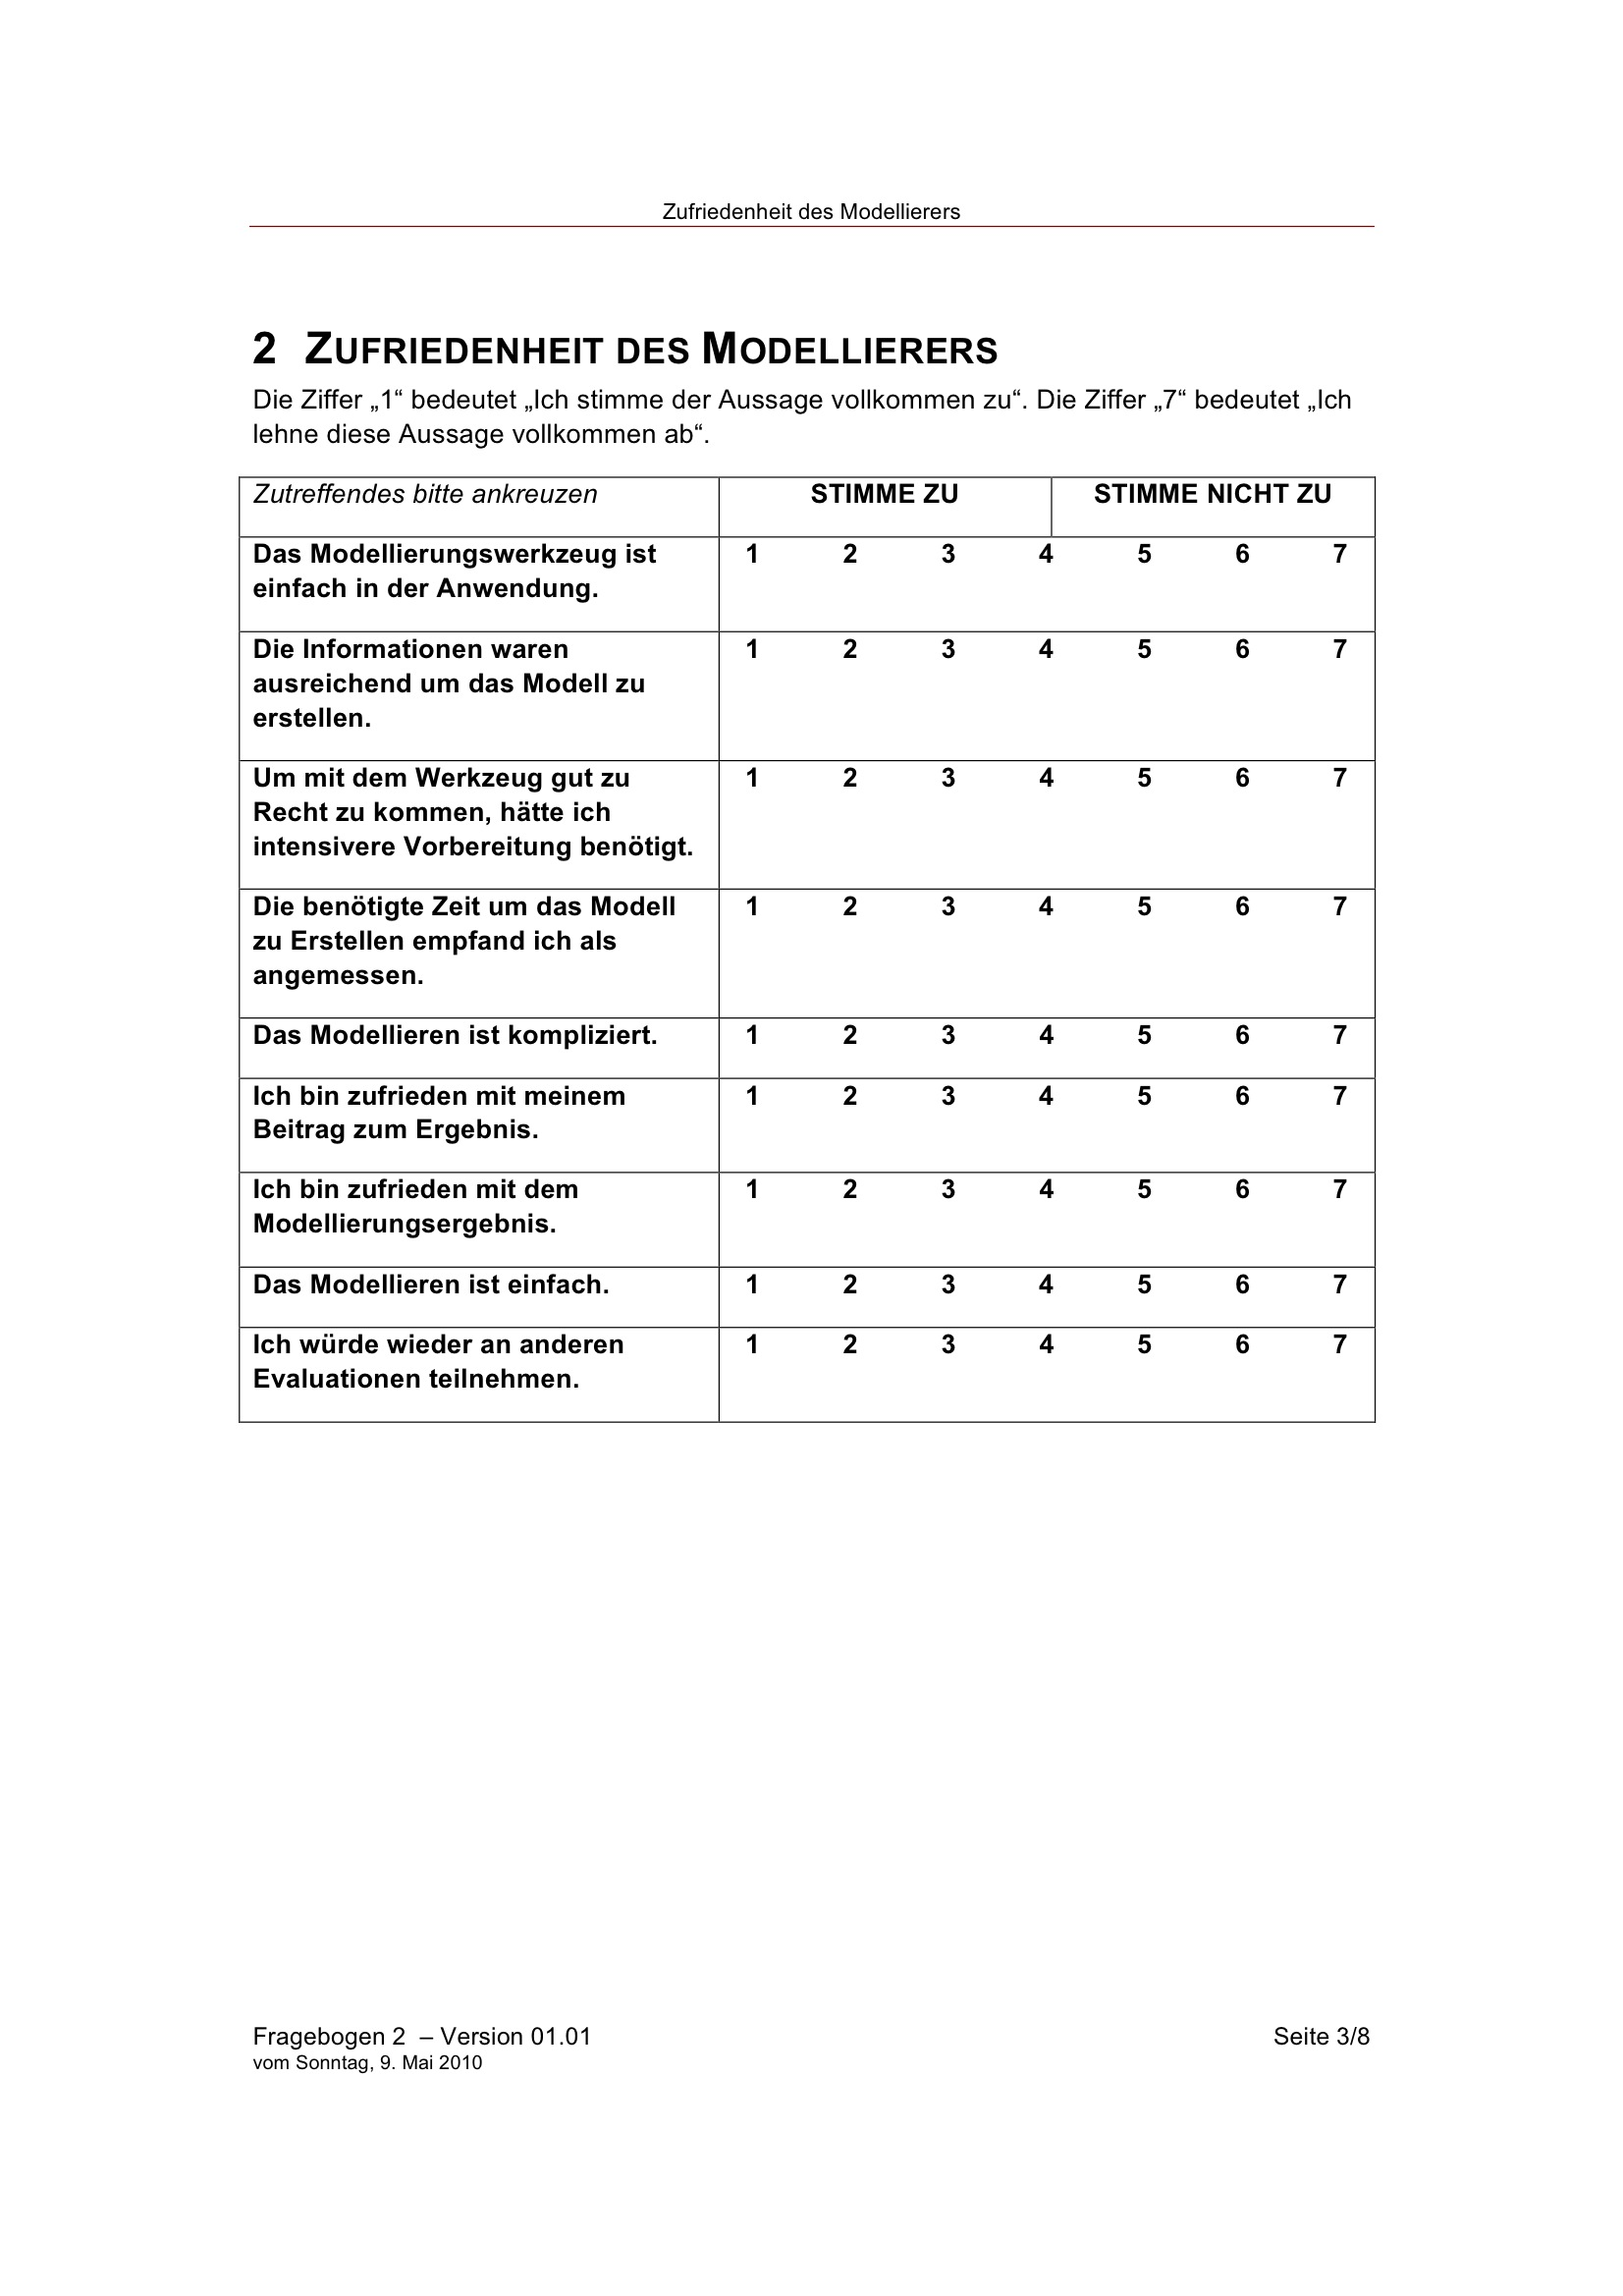
\includegraphics[width=0.9\textwidth]{img/AnhangEmpirie/fb4_1-03.jpeg}%
	}
	\caption{Erster Fragebogen für Evaluierungsblock 4 - Seite 3}
	\label{fig:img_AnhangEmpirie_fb4_1-03}
\end{figure}

\begin{figure}[htbp]
	\centering
	\fbox{%
		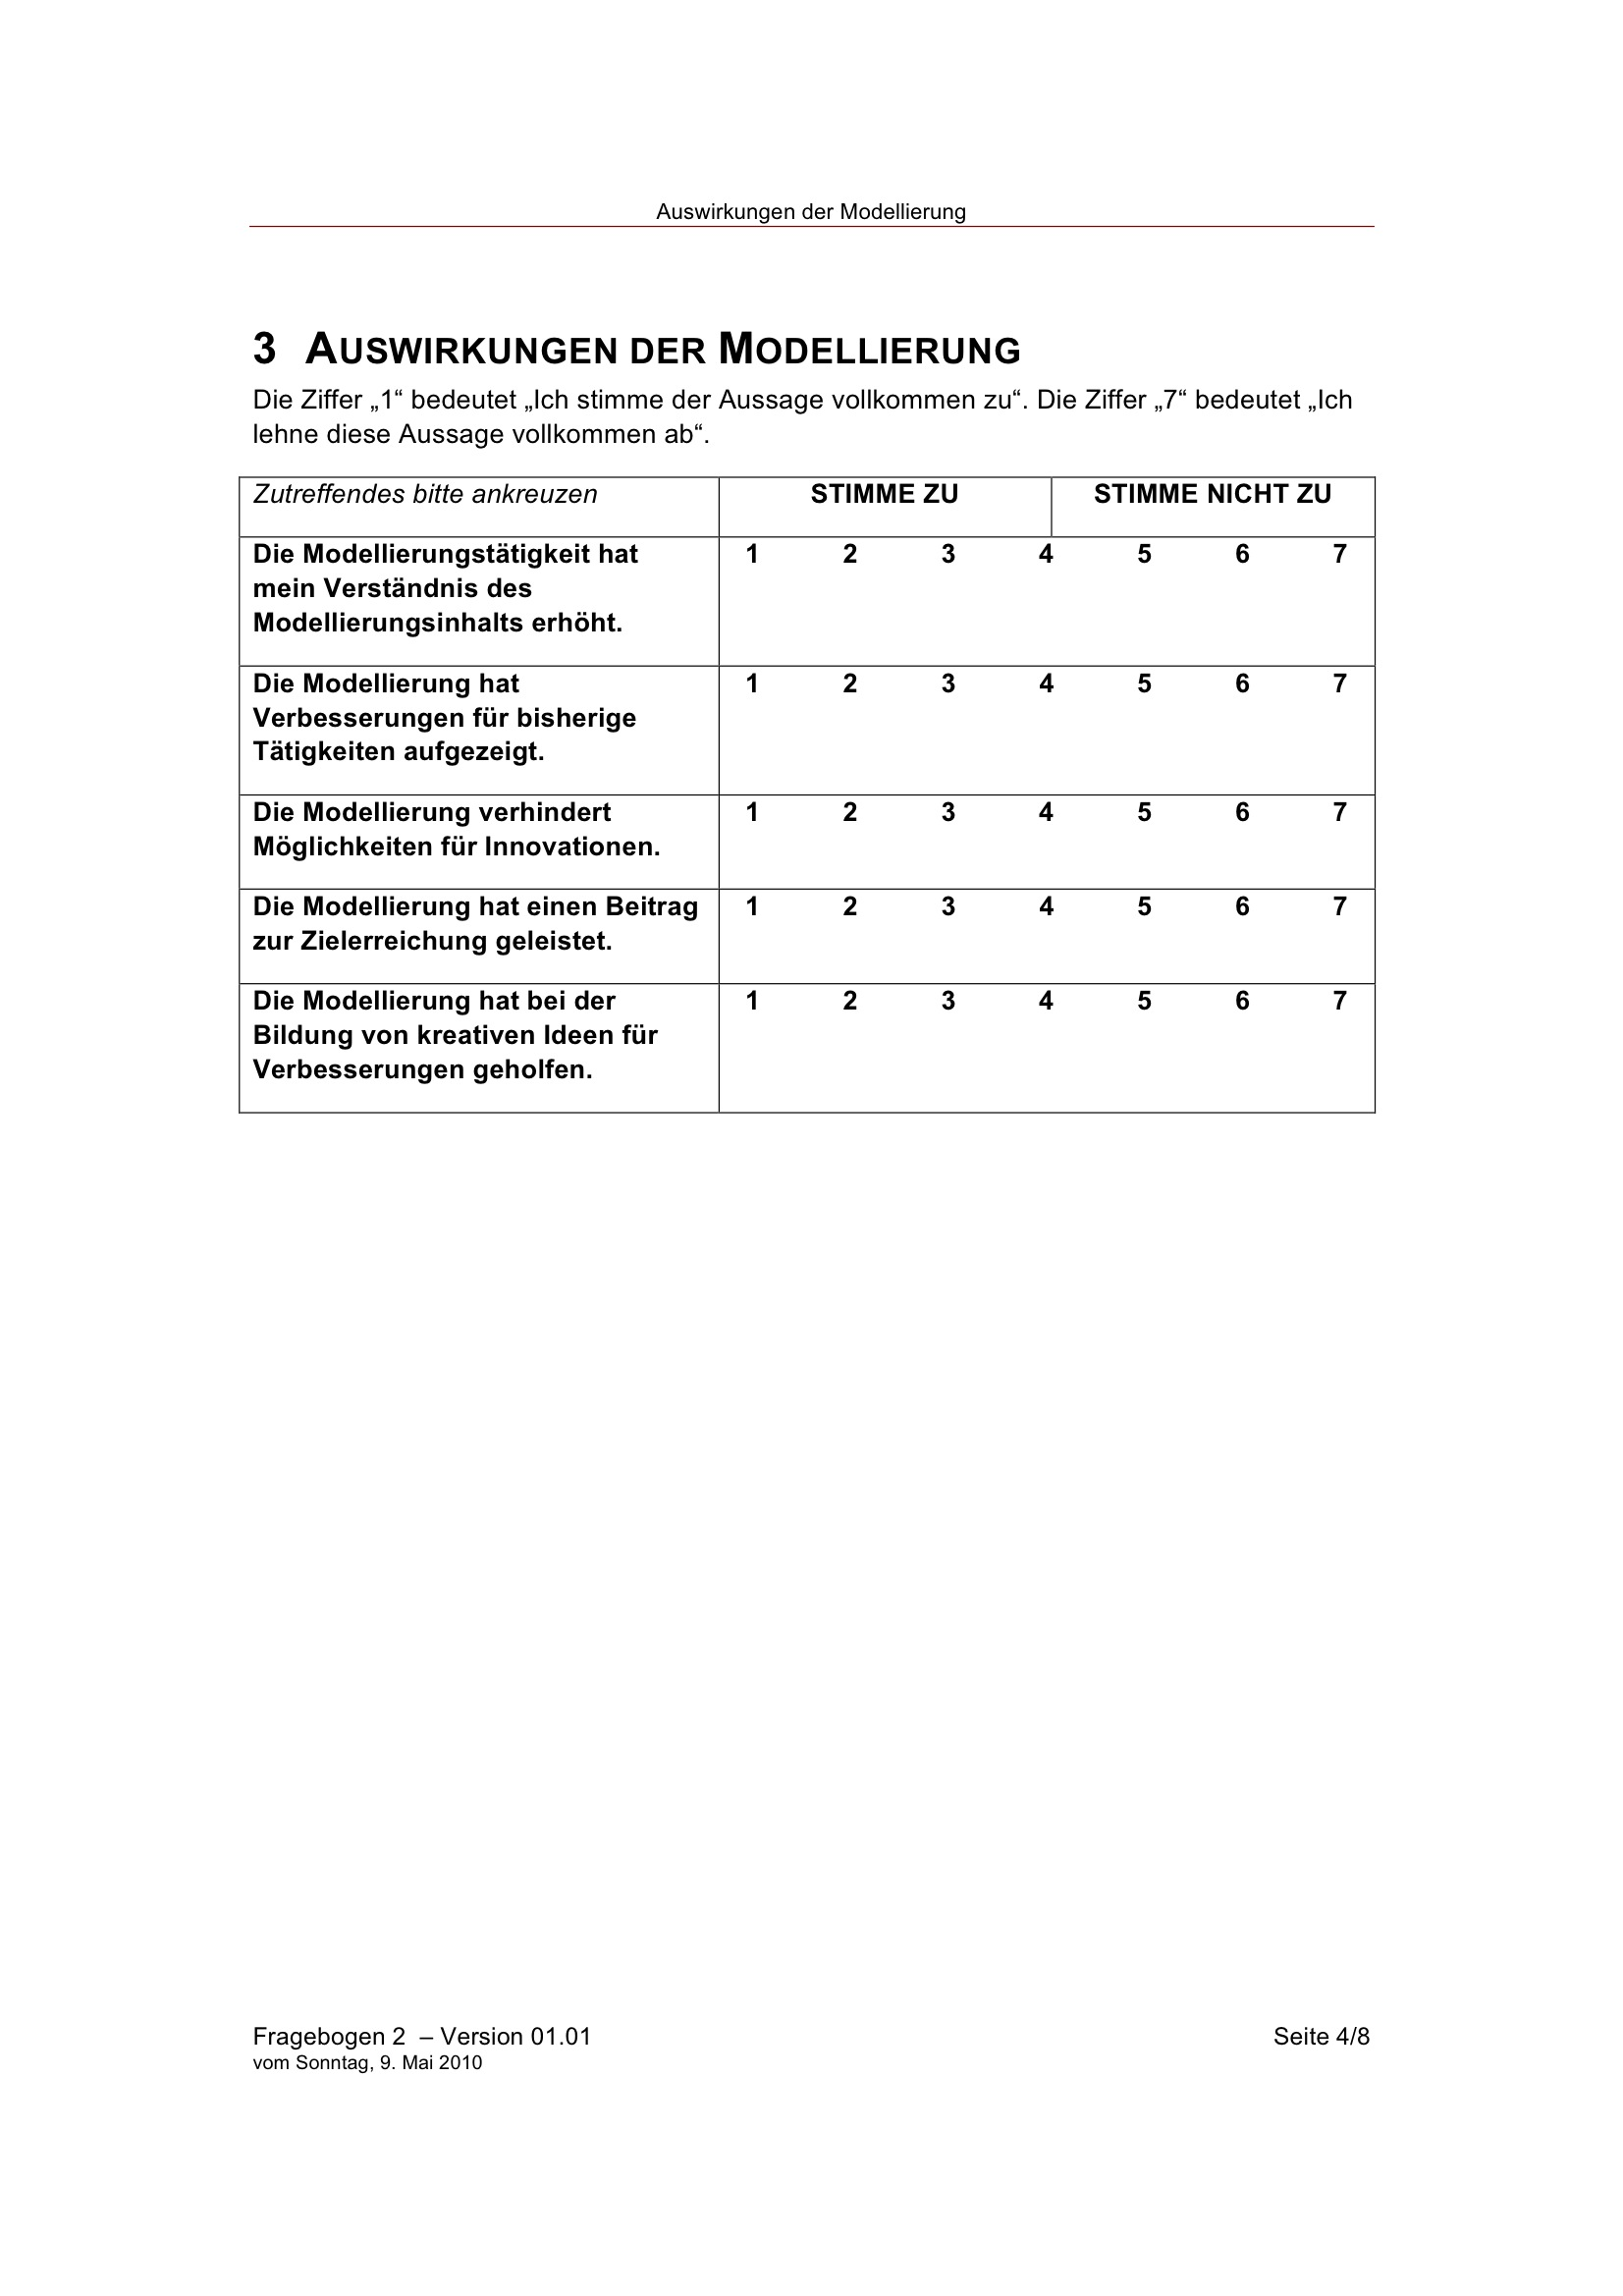
\includegraphics[width=0.9\textwidth]{img/AnhangEmpirie/fb4_1-04.jpeg}%
	}
	\caption{Erster Fragebogen für Evaluierungsblock 4 - Seite 4}
	\label{fig:img_AnhangEmpirie_fb4_1-04}
\end{figure}

\begin{figure}[htbp]
	\centering
	\fbox{%
		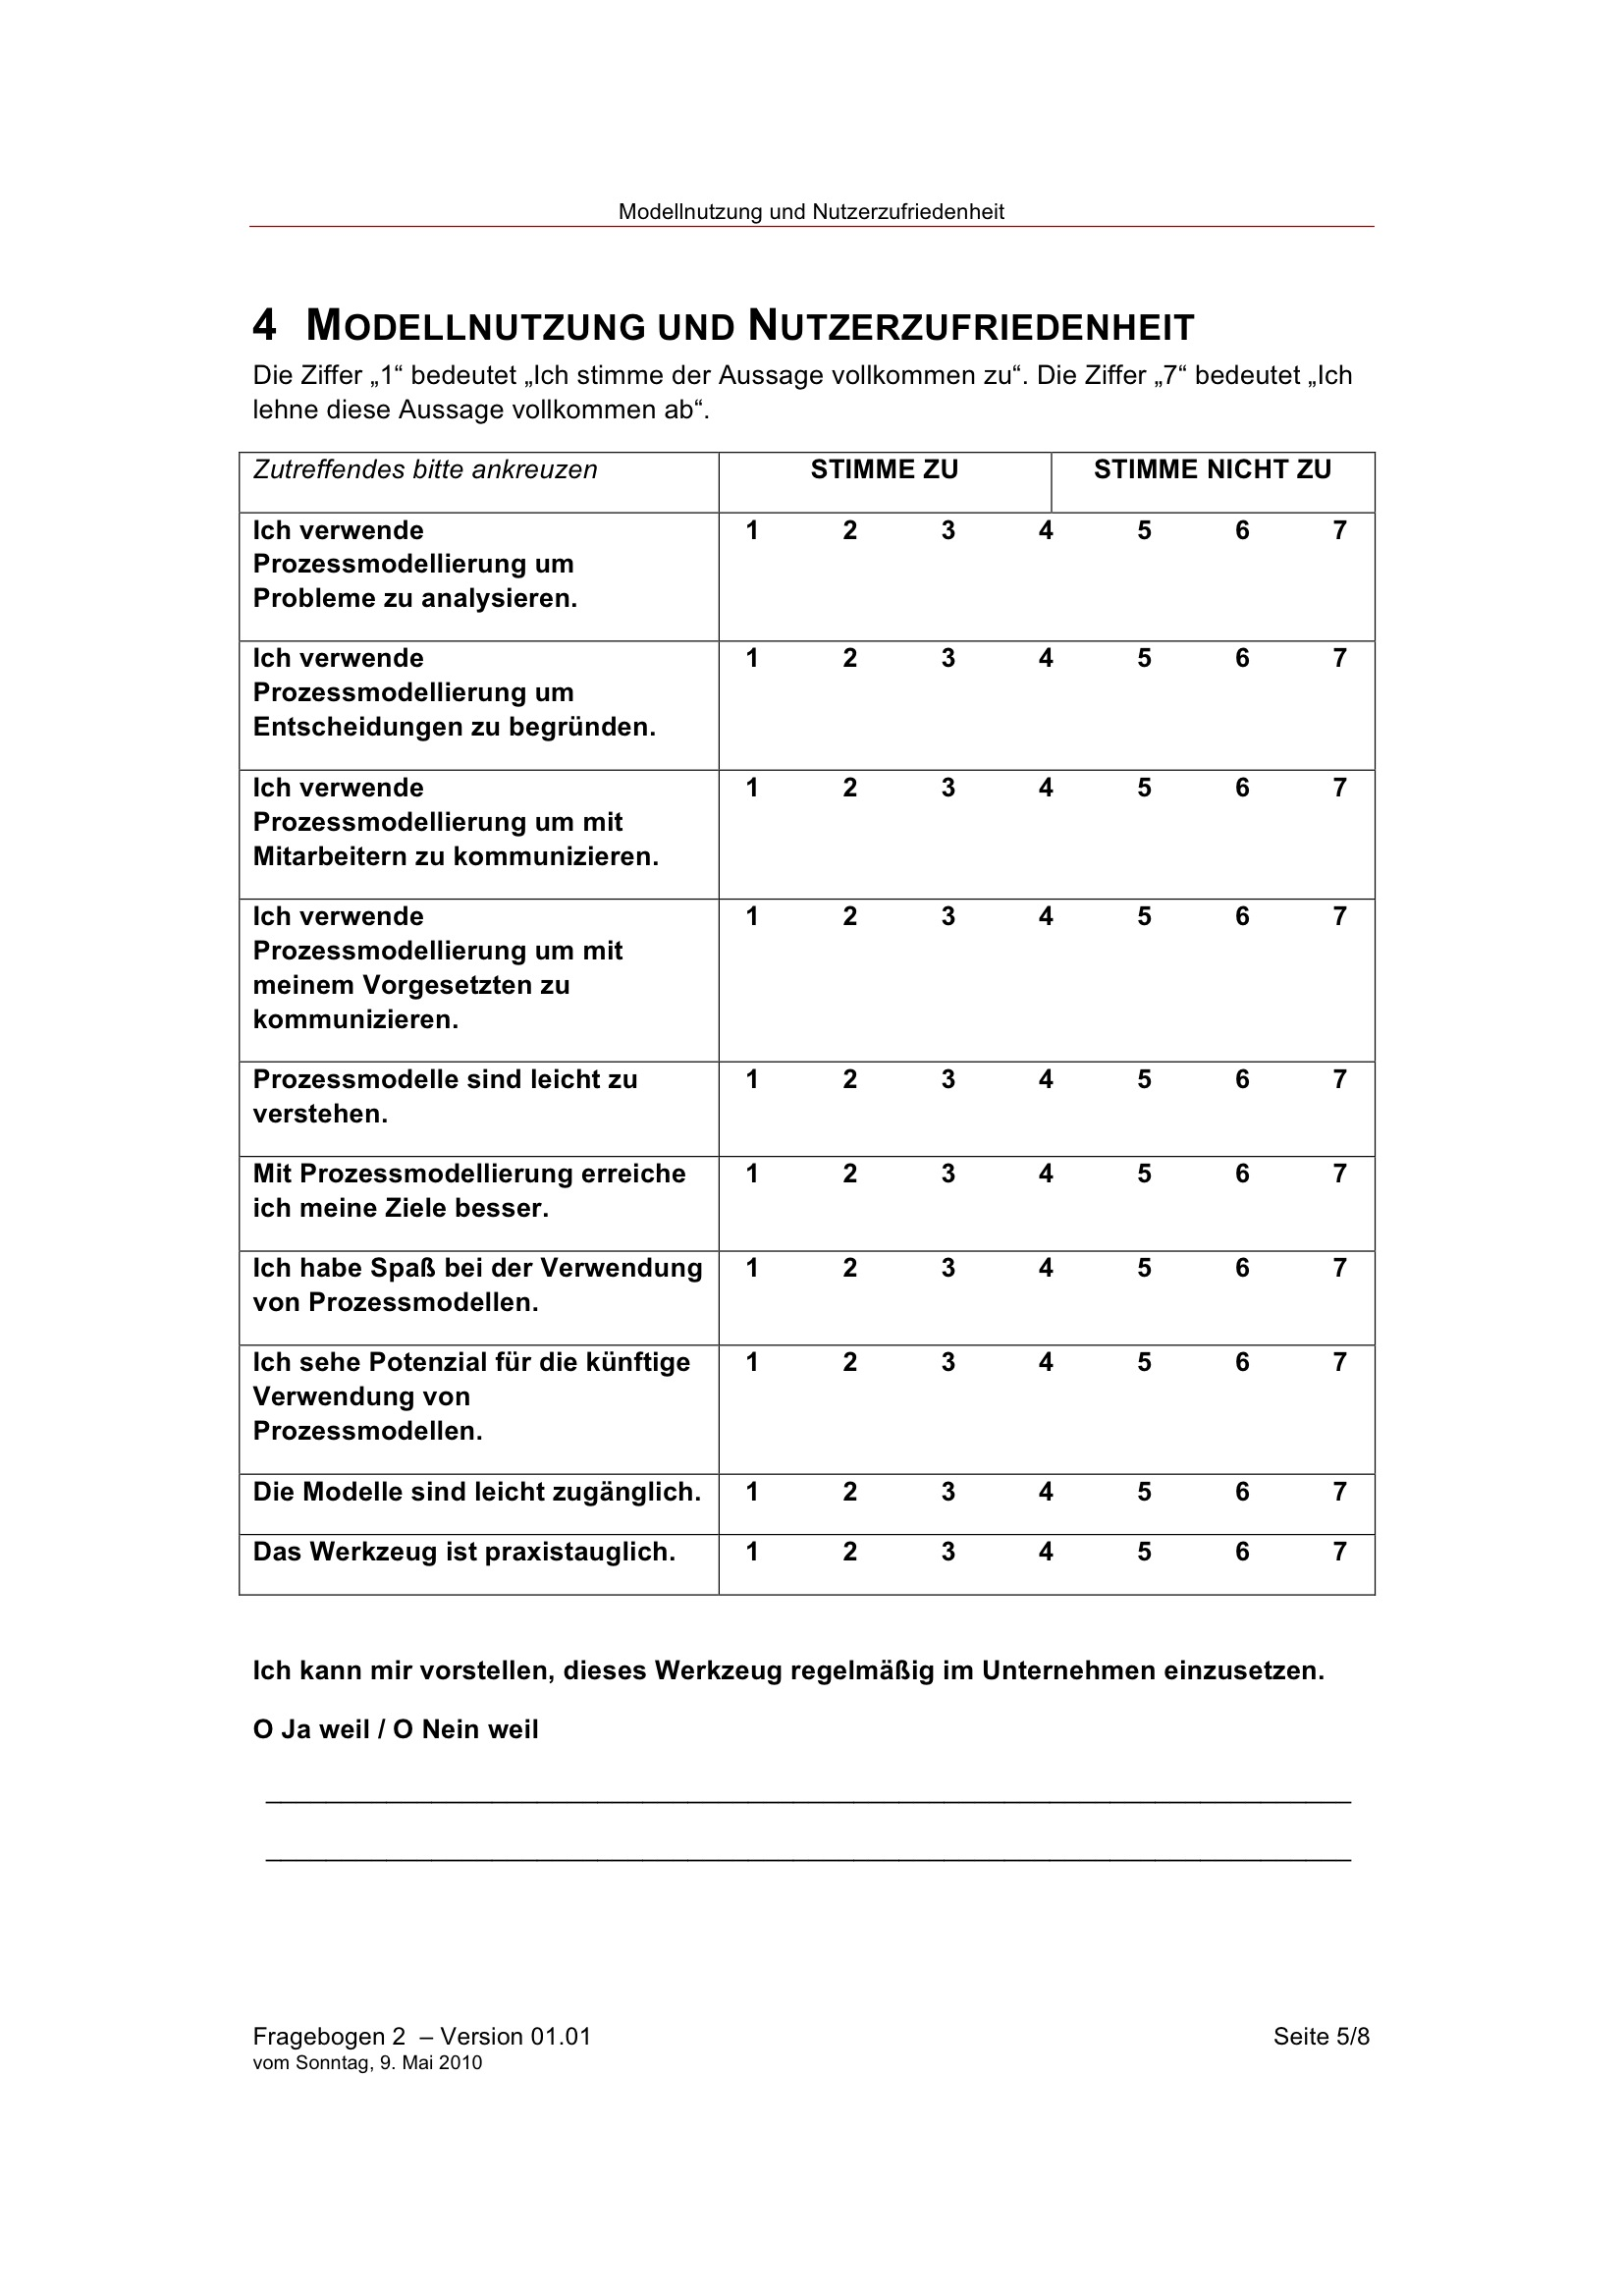
\includegraphics[width=0.9\textwidth]{img/AnhangEmpirie/fb4_1-05.jpeg}%
	}
	\caption{Erster Fragebogen für Evaluierungsblock 4 - Seite 5}
	\label{fig:img_AnhangEmpirie_fb4_1-05}
\end{figure}

\begin{figure}[htbp]
	\centering
	\fbox{%
		
\includegraphics[width=0.9\textwidth]{img/AnhangEmpirie/fb4_1-06.jpeg}%
	}
	\caption{Erster Fragebogen für Evaluierungsblock 4 - Seite 6}
	\label{fig:img_AnhangEmpirie_fb4_1-06}
\end{figure}

\begin{figure}[htbp]
	\centering
	\fbox{%
		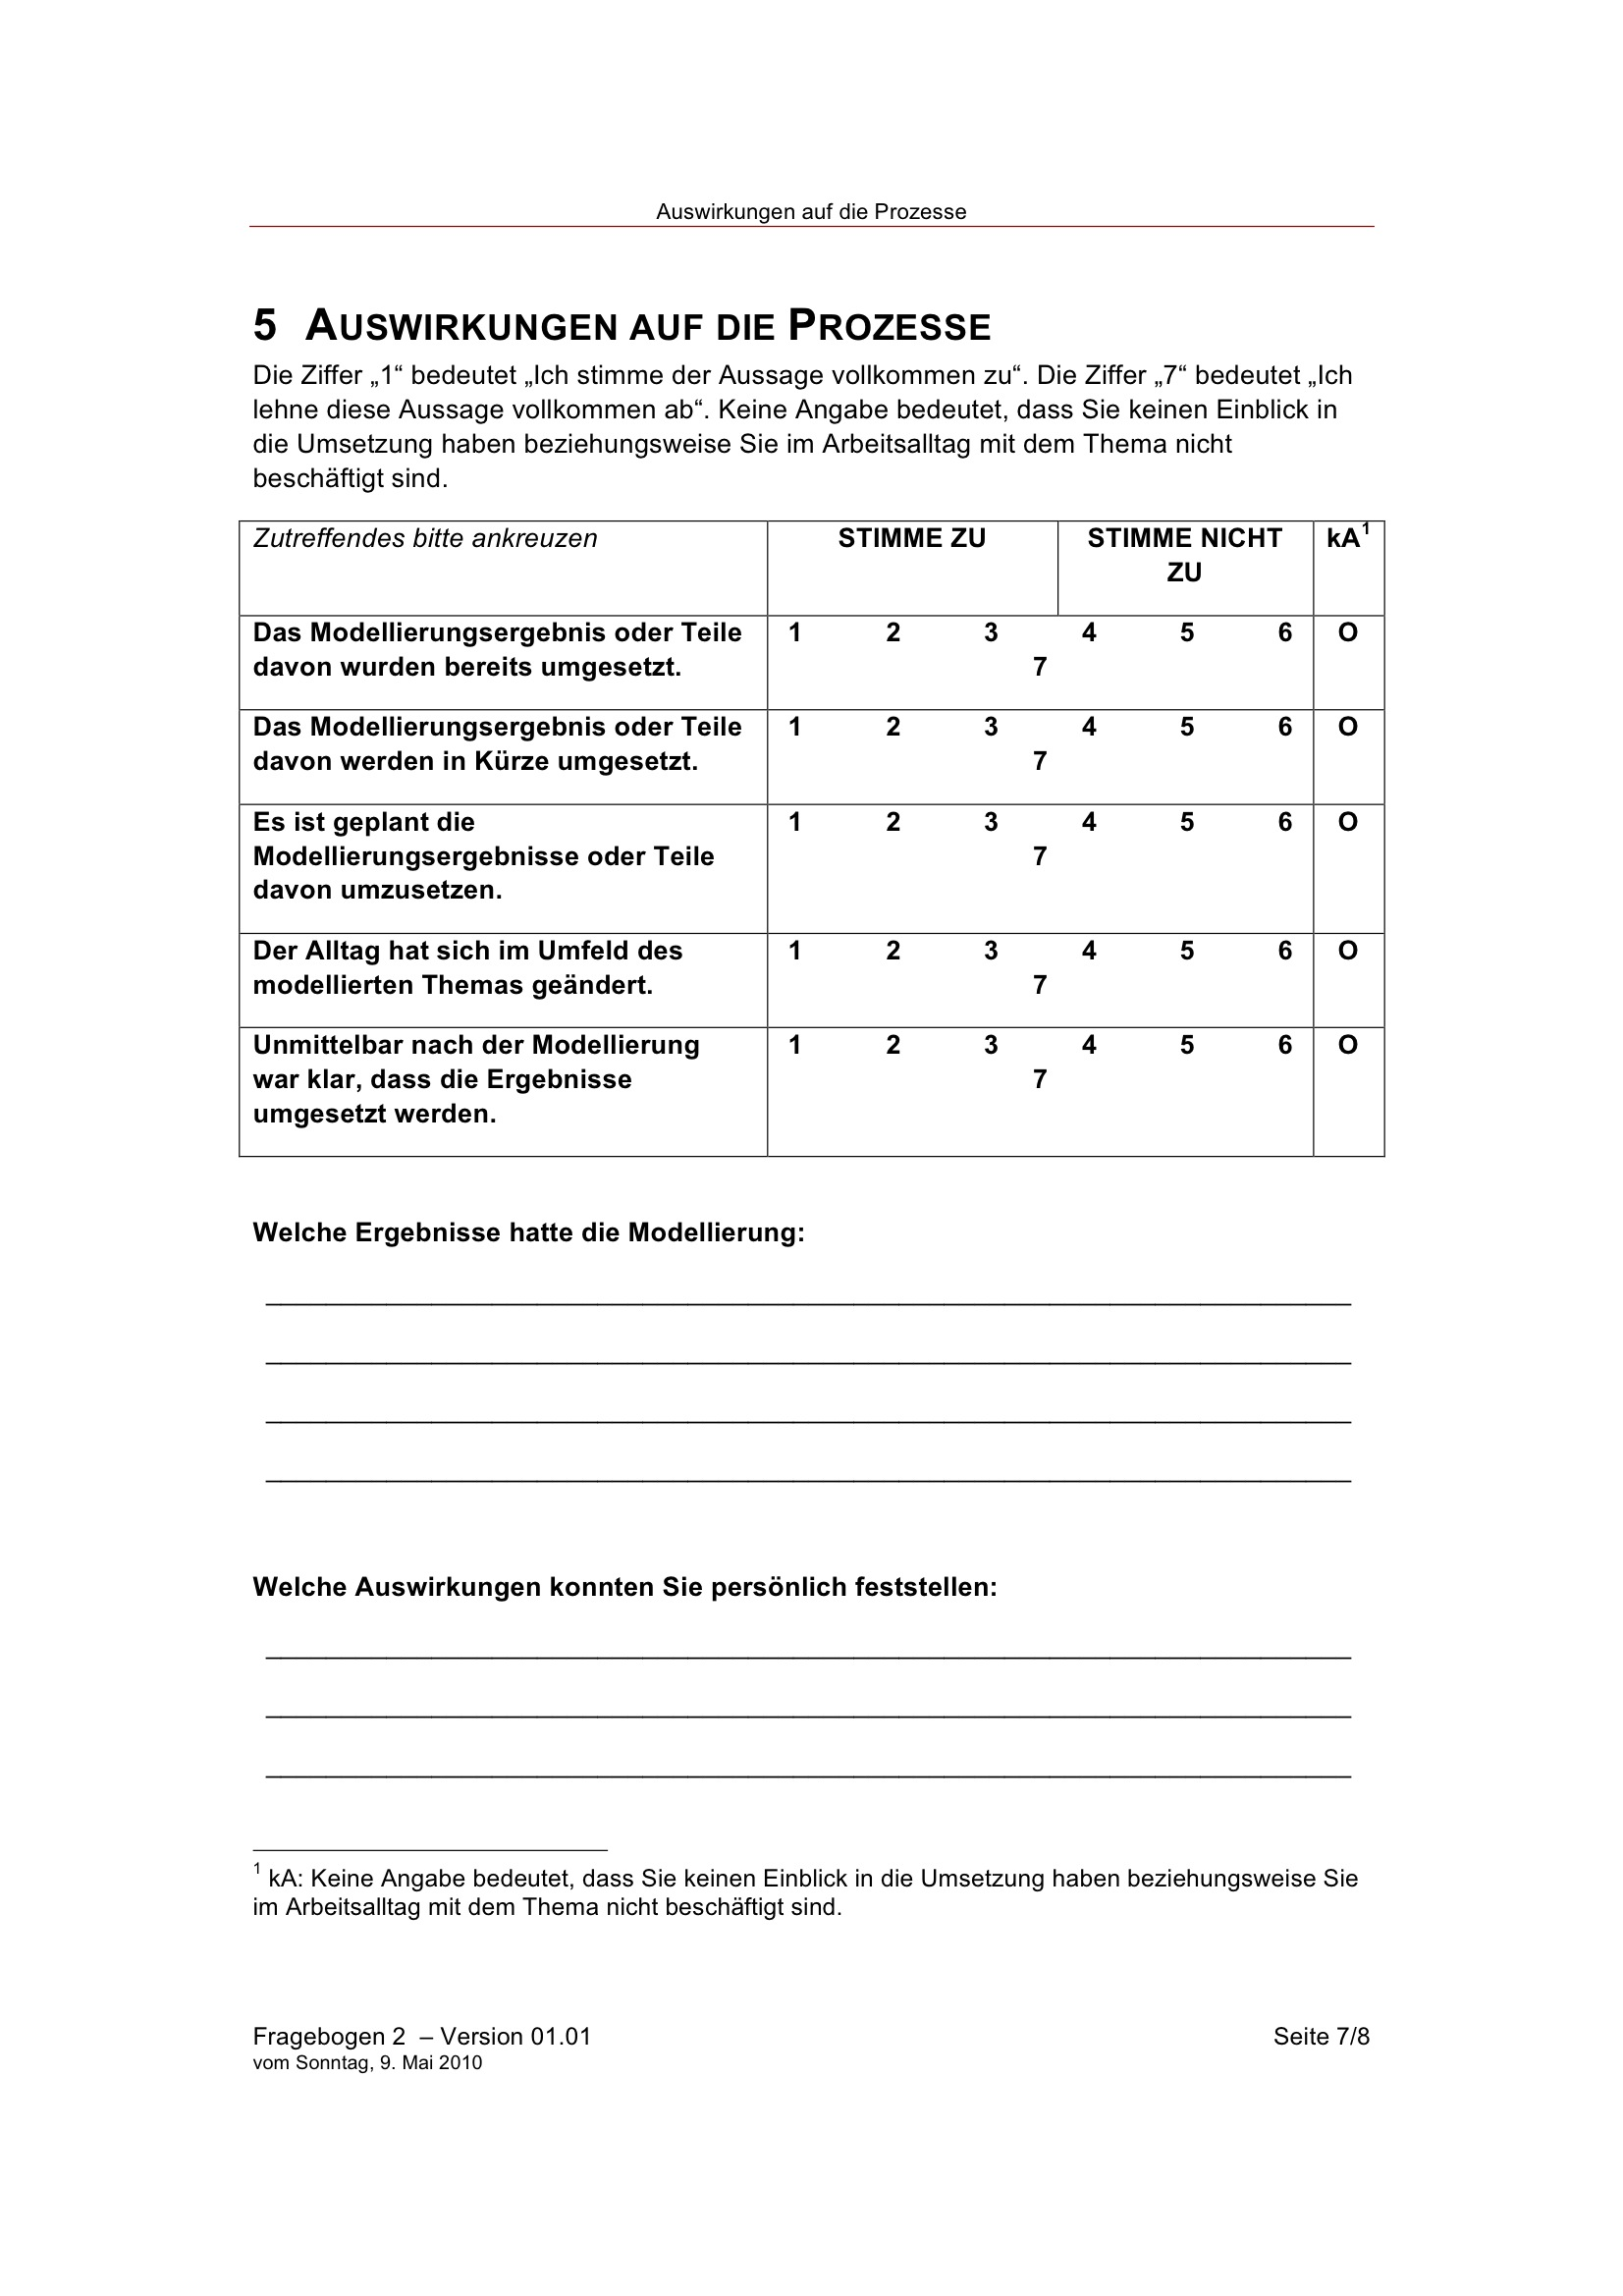
\includegraphics[width=0.9\textwidth]{img/AnhangEmpirie/fb4_1-07.jpeg}%
	}
	\caption{Erster Fragebogen für Evaluierungsblock 4 - Seite 7}
	\label{fig:img_AnhangEmpirie_fb4_1-07}
\end{figure}

\begin{figure}[htbp]
	\centering
	\fbox{%
		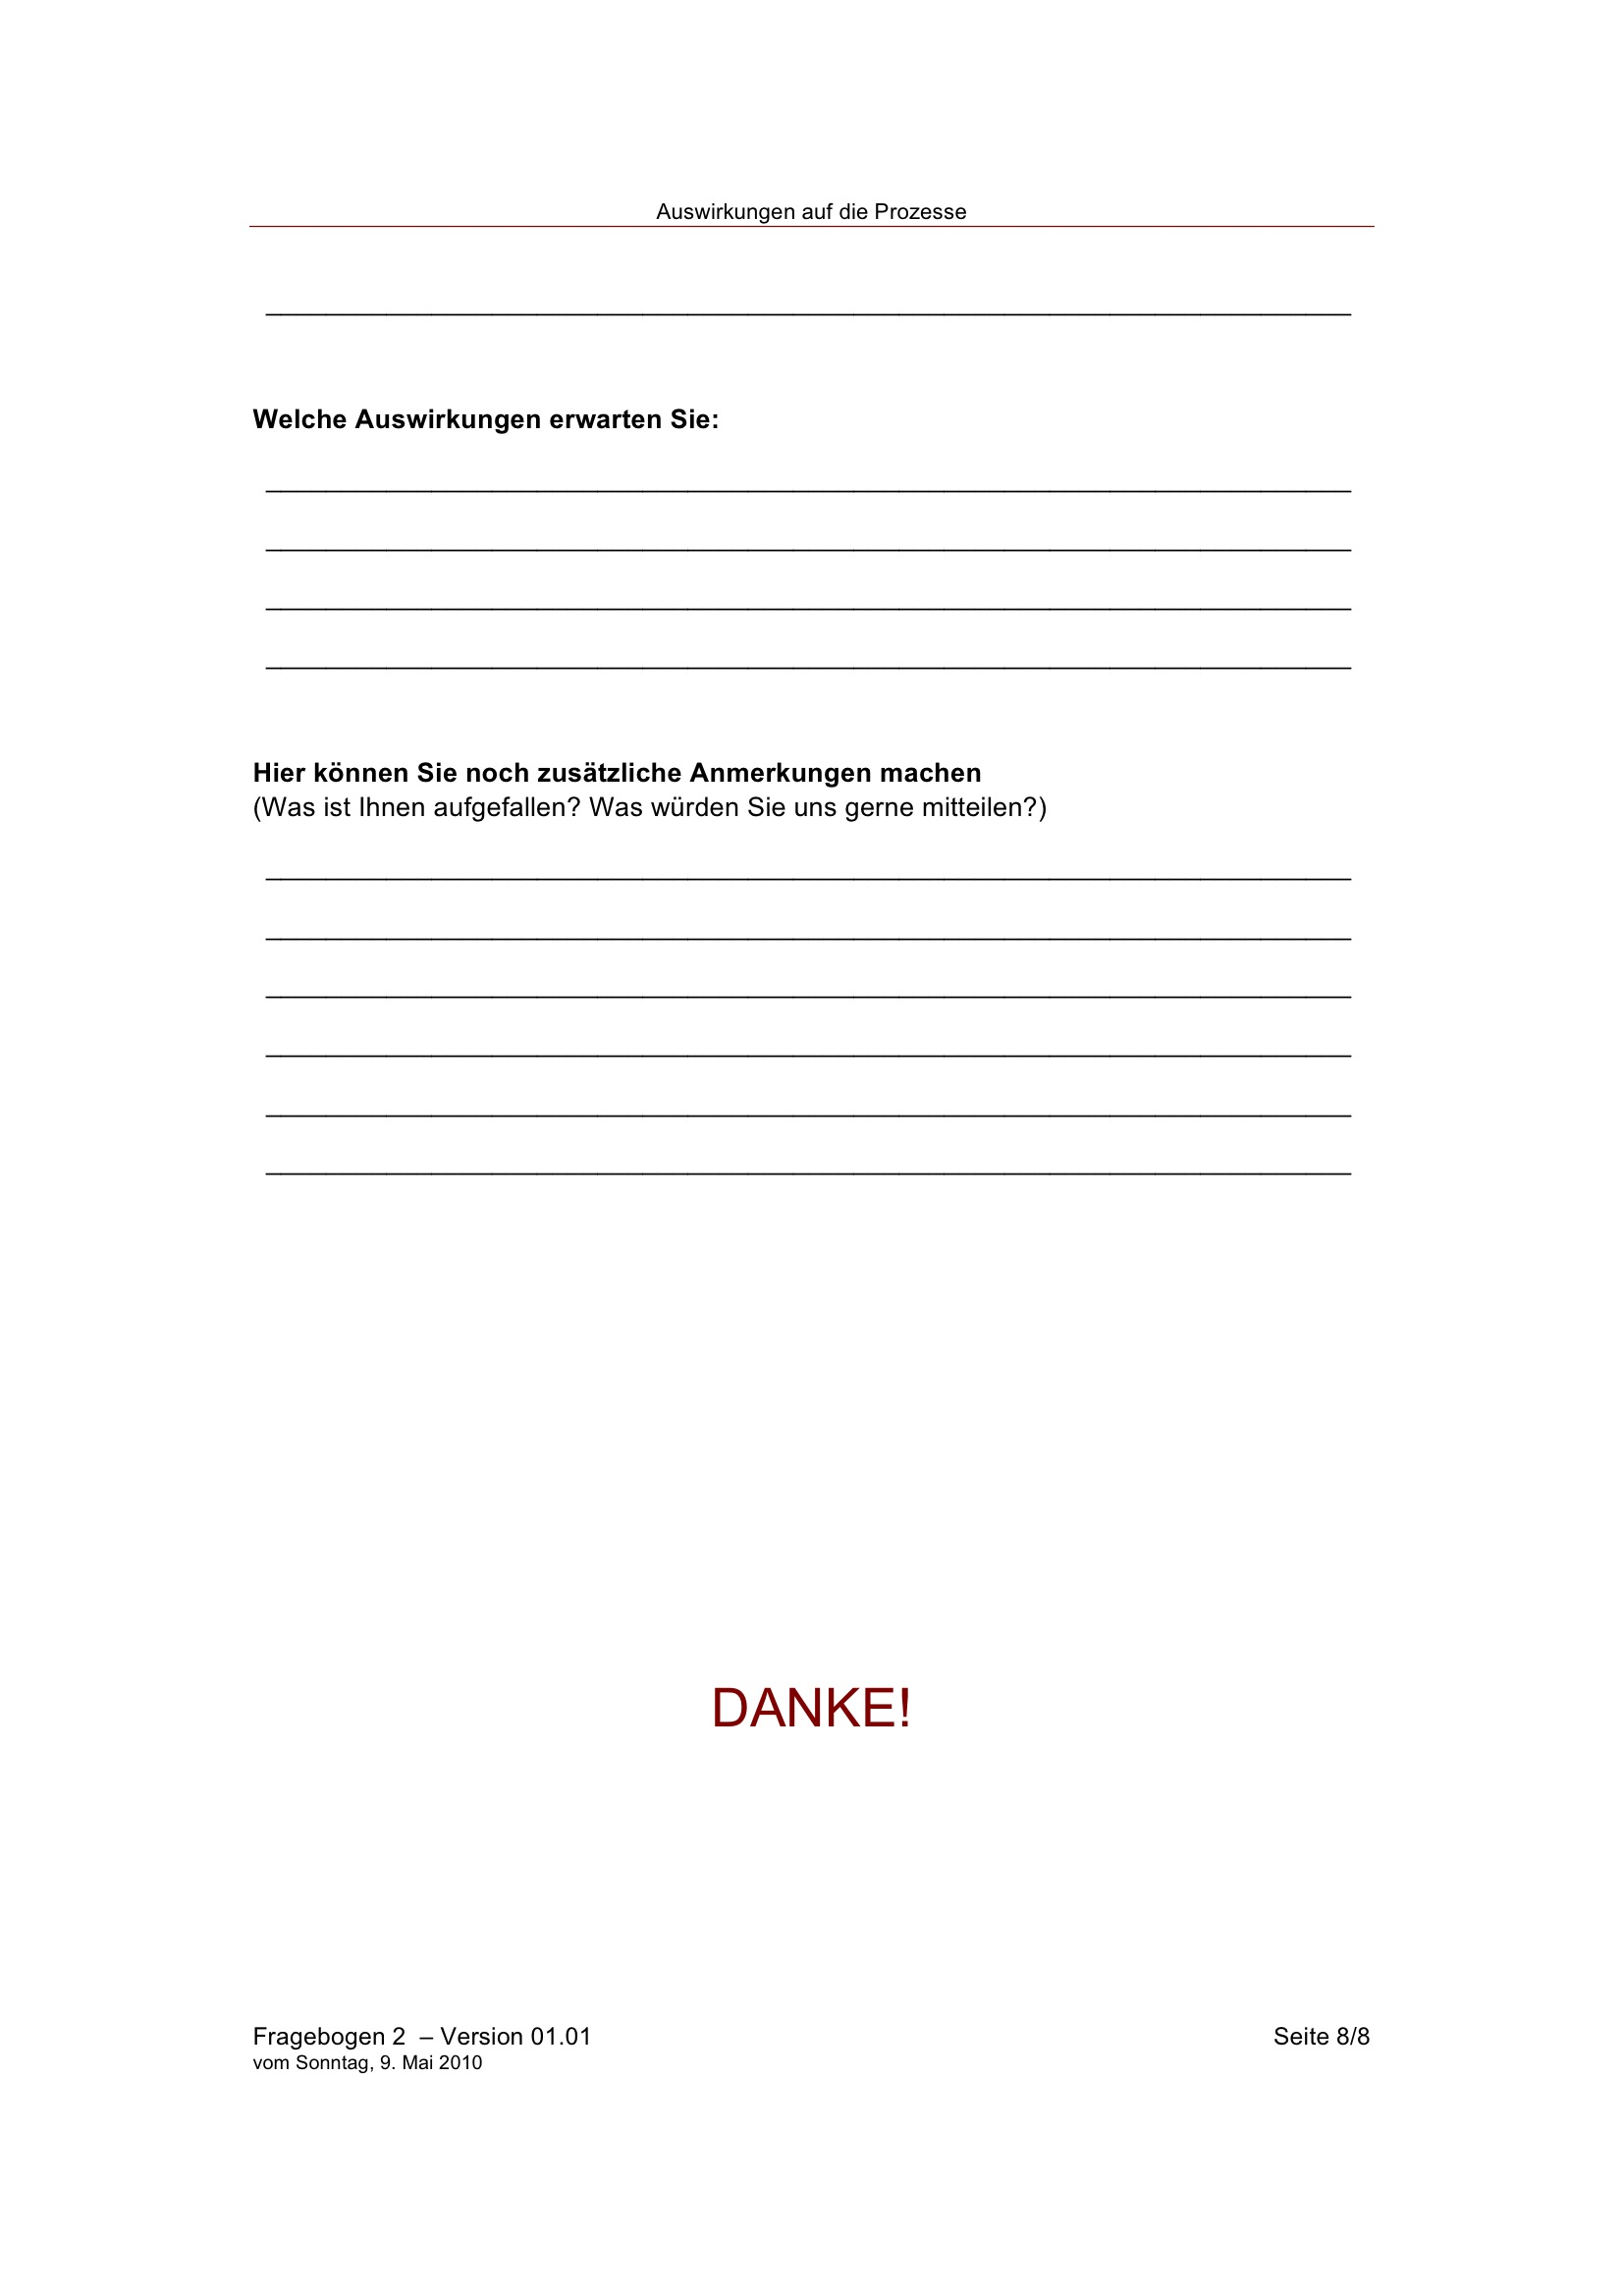
\includegraphics[width=0.9\textwidth]{img/AnhangEmpirie/fb4_1-08.jpeg}%
	}
	\caption{Erster Fragebogen für Evaluierungsblock 4 - Seite 8}
	\label{fig:img_AnhangEmpirie_fb4_1-08}
\end{figure}

\begin{figure}[htbp]
	\centering
	\fbox{%
		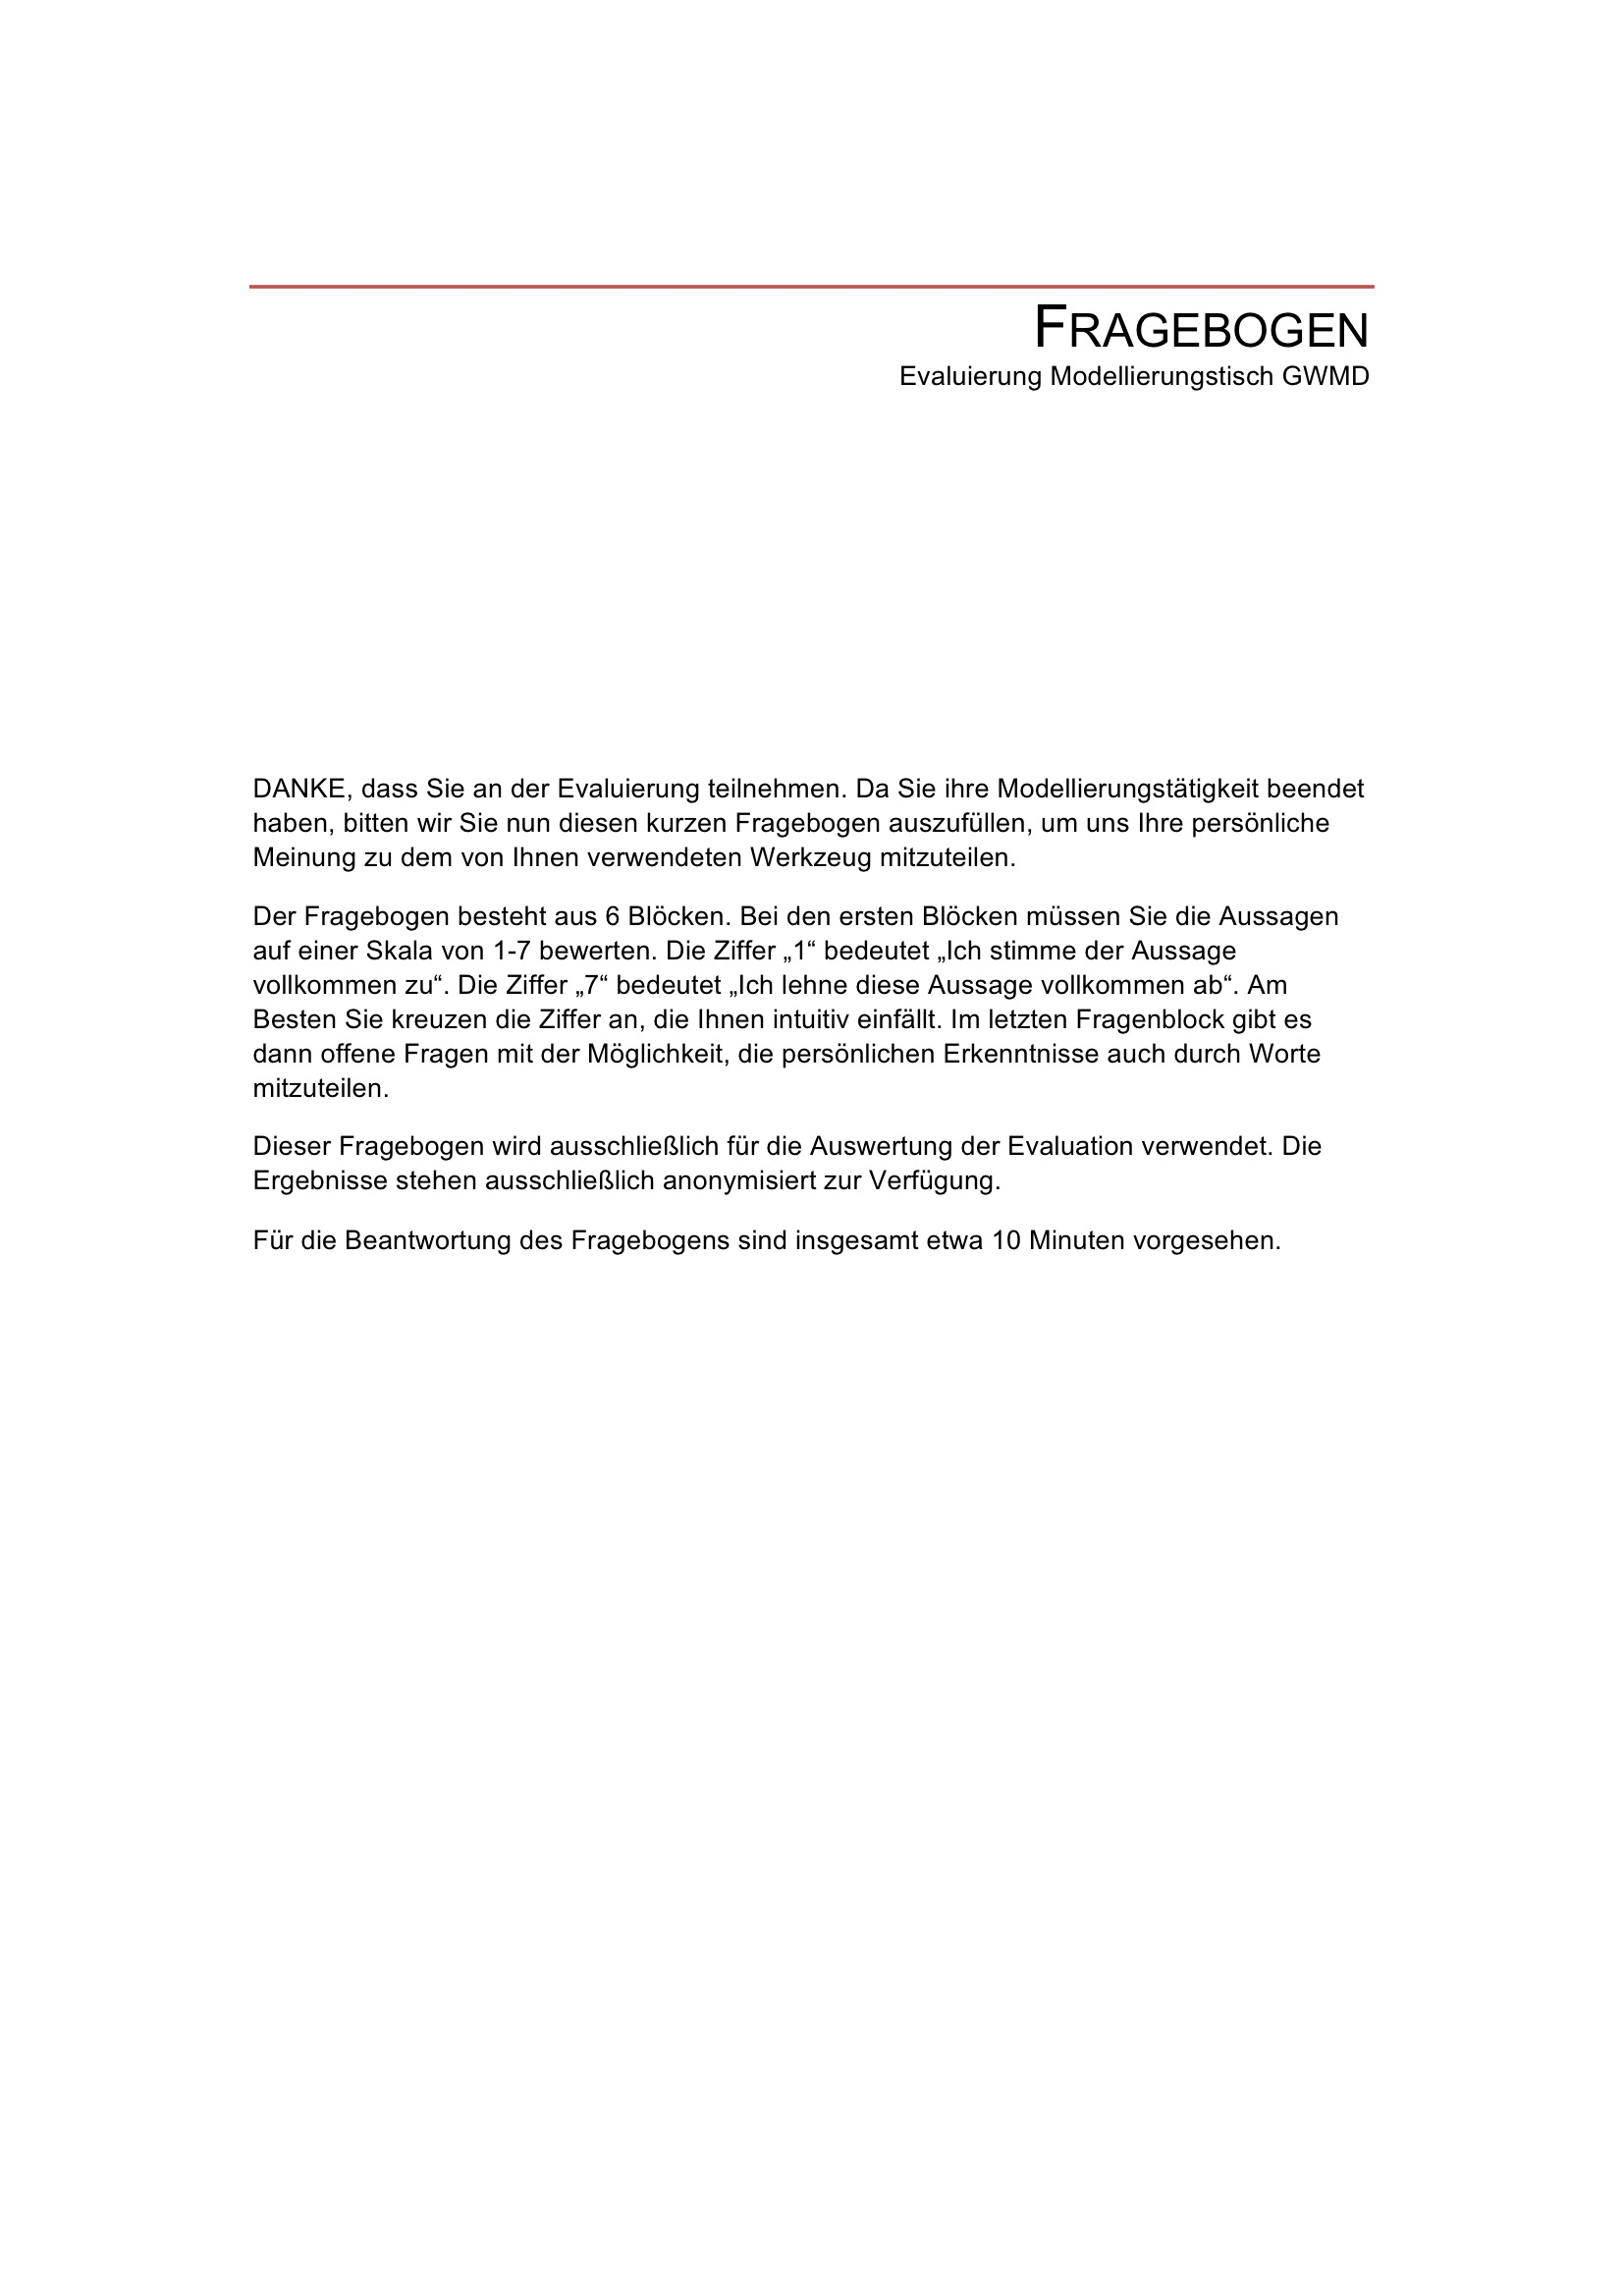
\includegraphics[width=0.9\textwidth]{img/AnhangEmpirie/fb4_2-01.jpeg}%
	}
	\caption{Zweiter Fragebogen für Evaluierungsblock 4 - Seite 1}
	\label{fig:img_AnhangEmpirie_fb4_2-01}
\end{figure}

\begin{figure}[htbp]
	\centering
	\fbox{%
		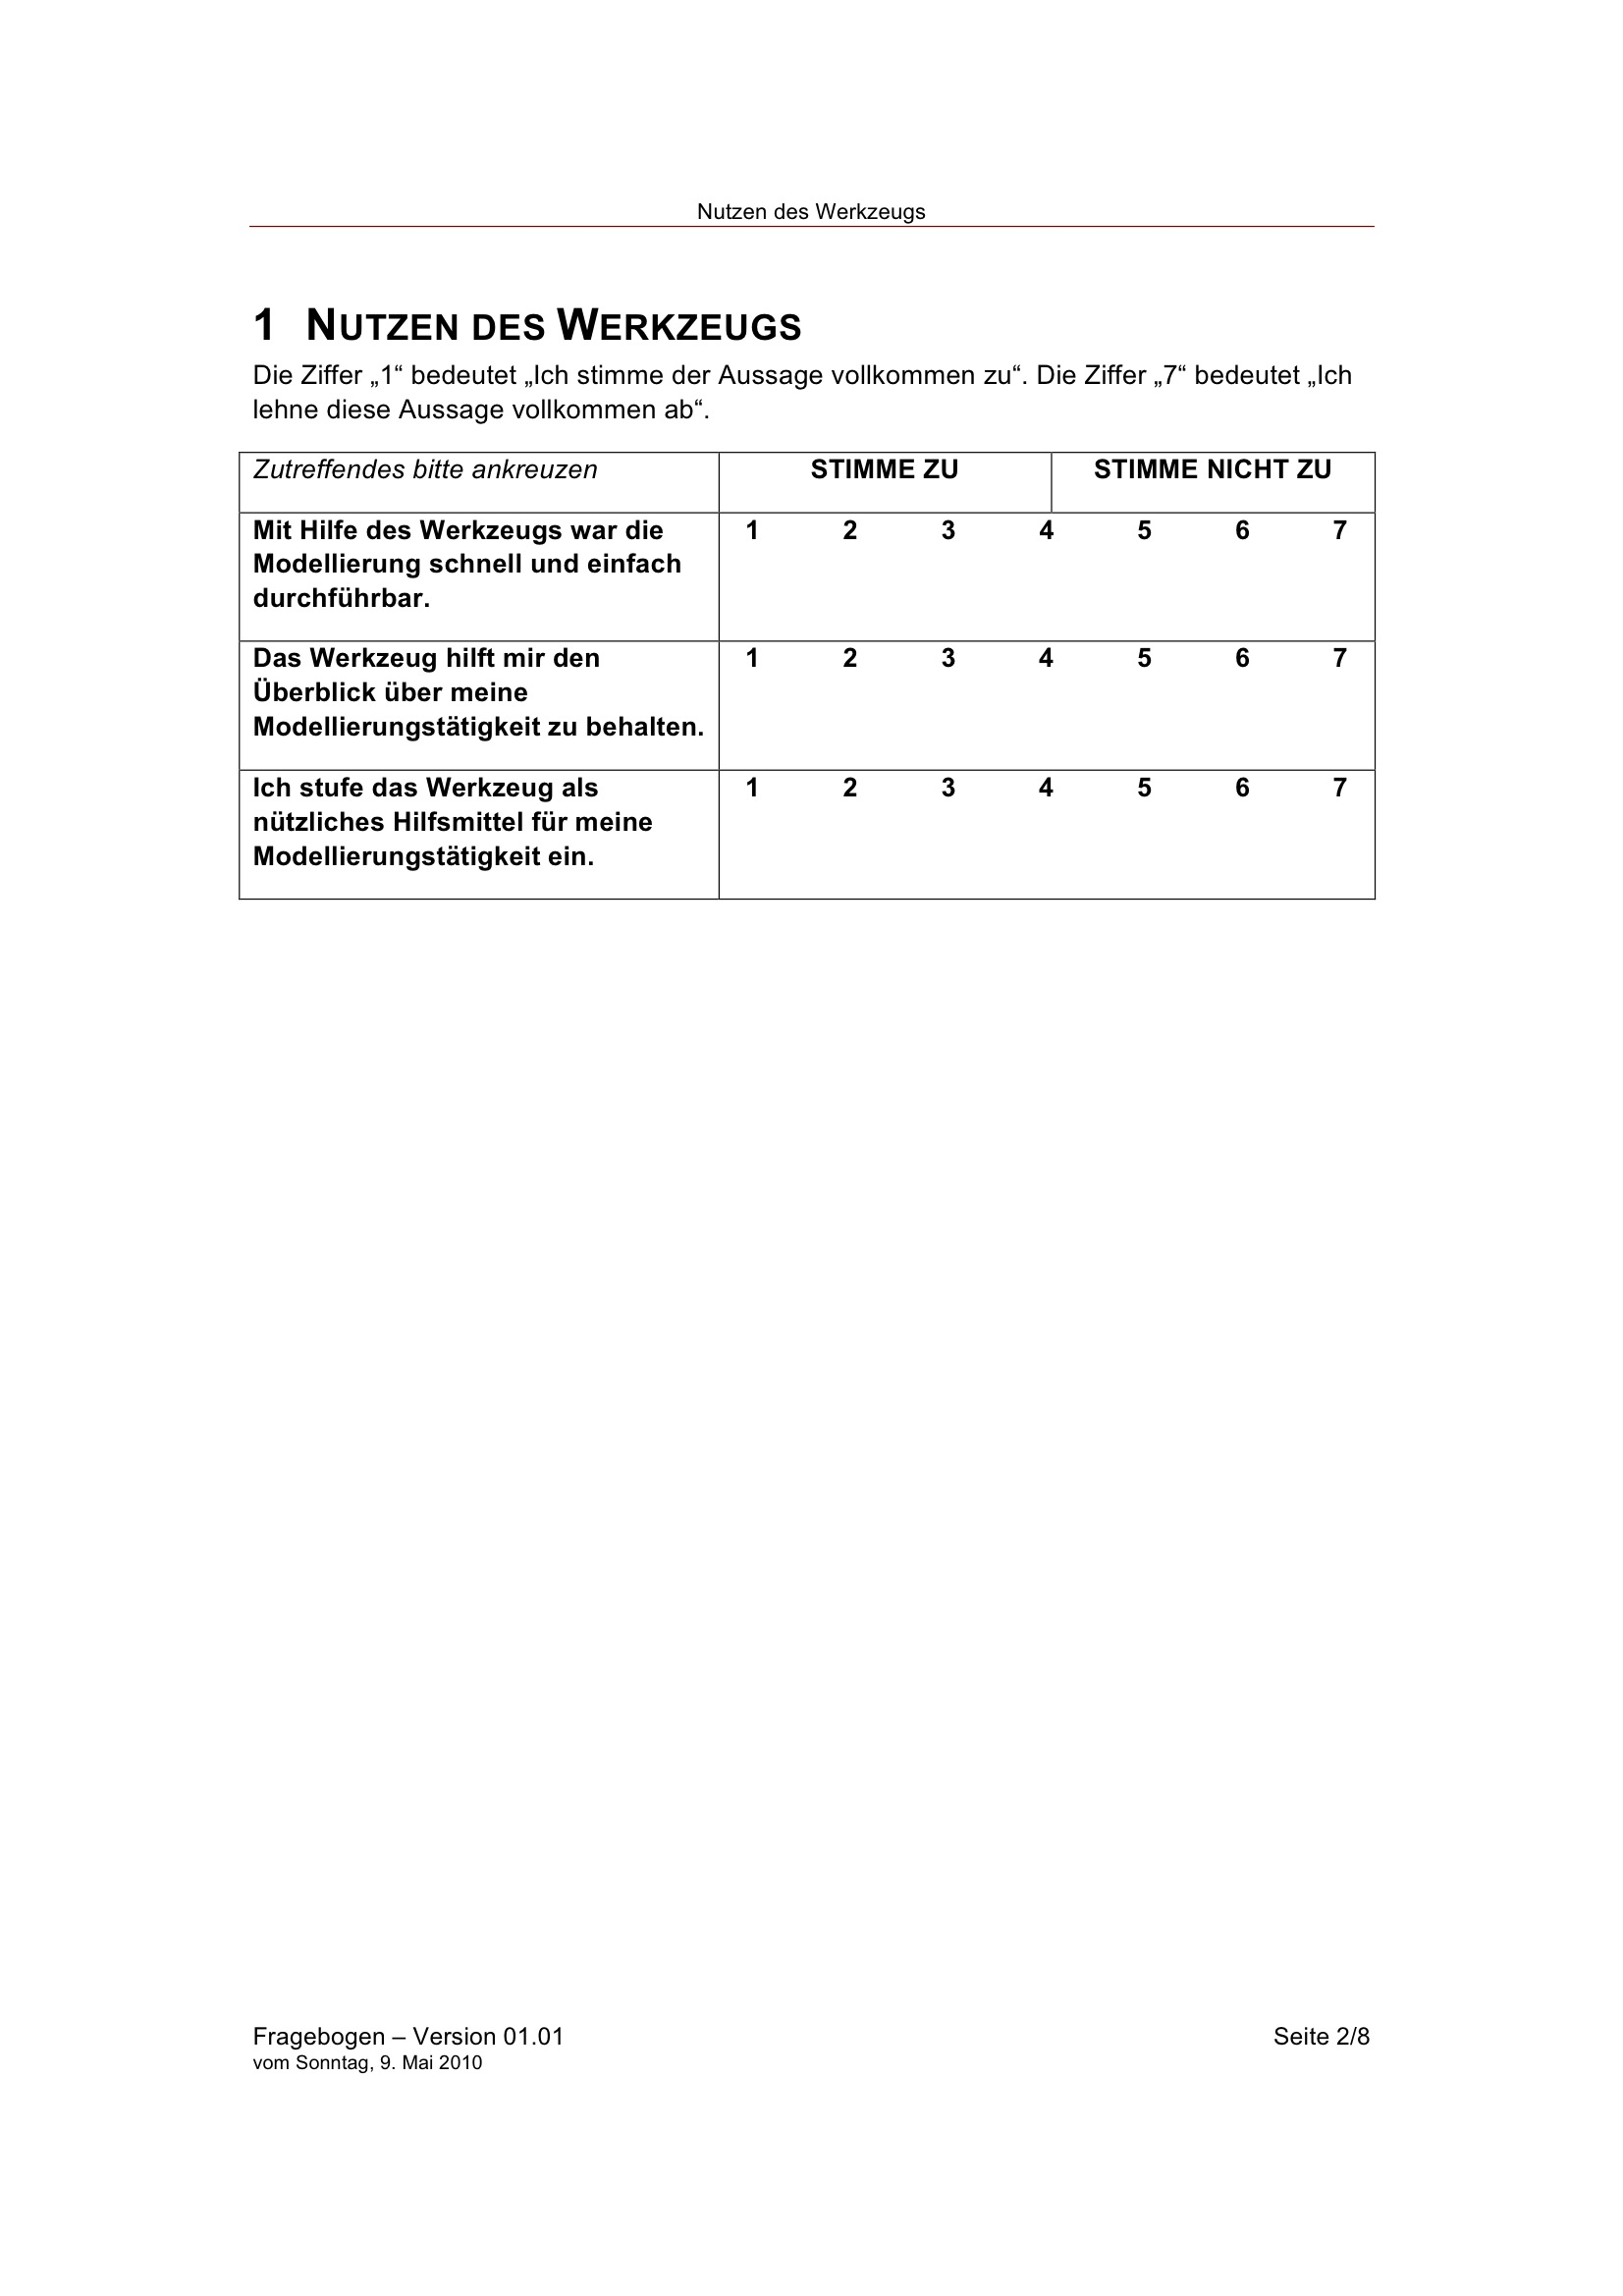
\includegraphics[width=0.9\textwidth]{img/AnhangEmpirie/fb4_2-02.jpeg}%
	}
	\caption{Zweiter Fragebogen für Evaluierungsblock 4 - Seite 2}
	\label{fig:img_AnhangEmpirie_fb4_2-02}
\end{figure}

\begin{figure}[htbp]
	\centering
	\fbox{%
		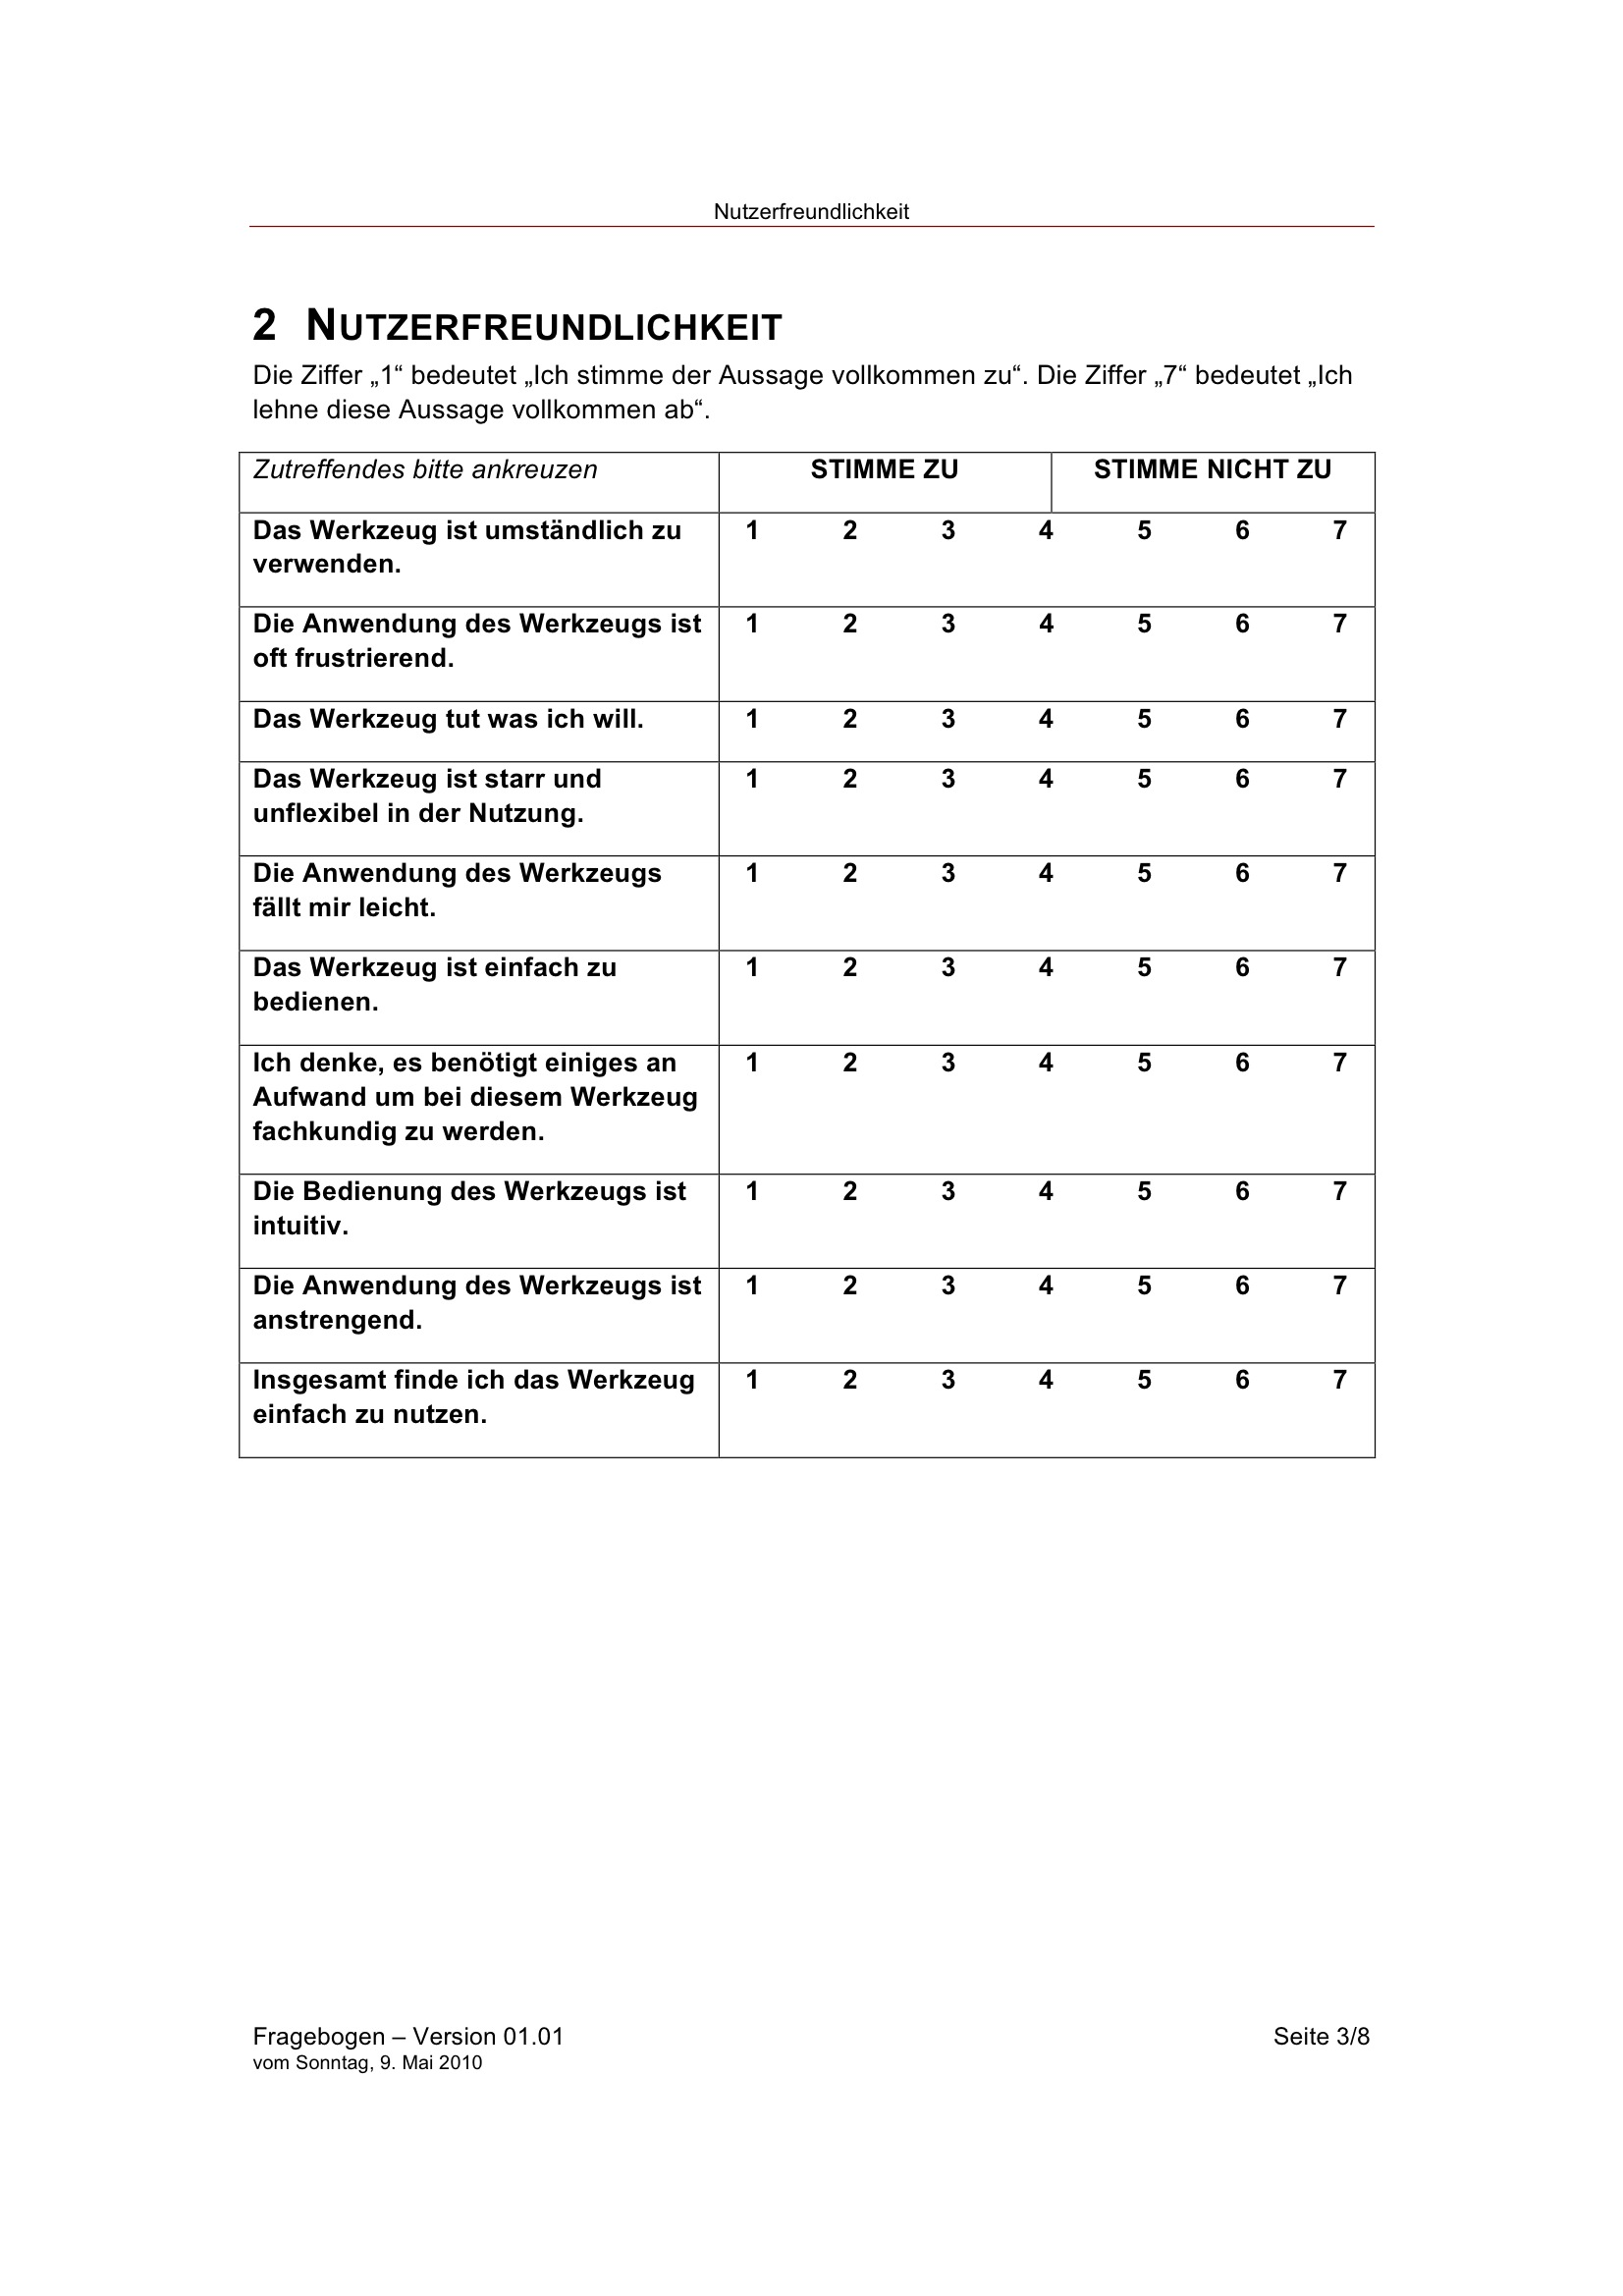
\includegraphics[width=0.9\textwidth]{img/AnhangEmpirie/fb4_2-03.jpeg}%
	}
	\caption{Zweiter Fragebogen für Evaluierungsblock 4 - Seite 3}
	\label{fig:img_AnhangEmpirie_fb4_2-03}
\end{figure}

\begin{figure}[htbp]
	\centering
	\fbox{%
		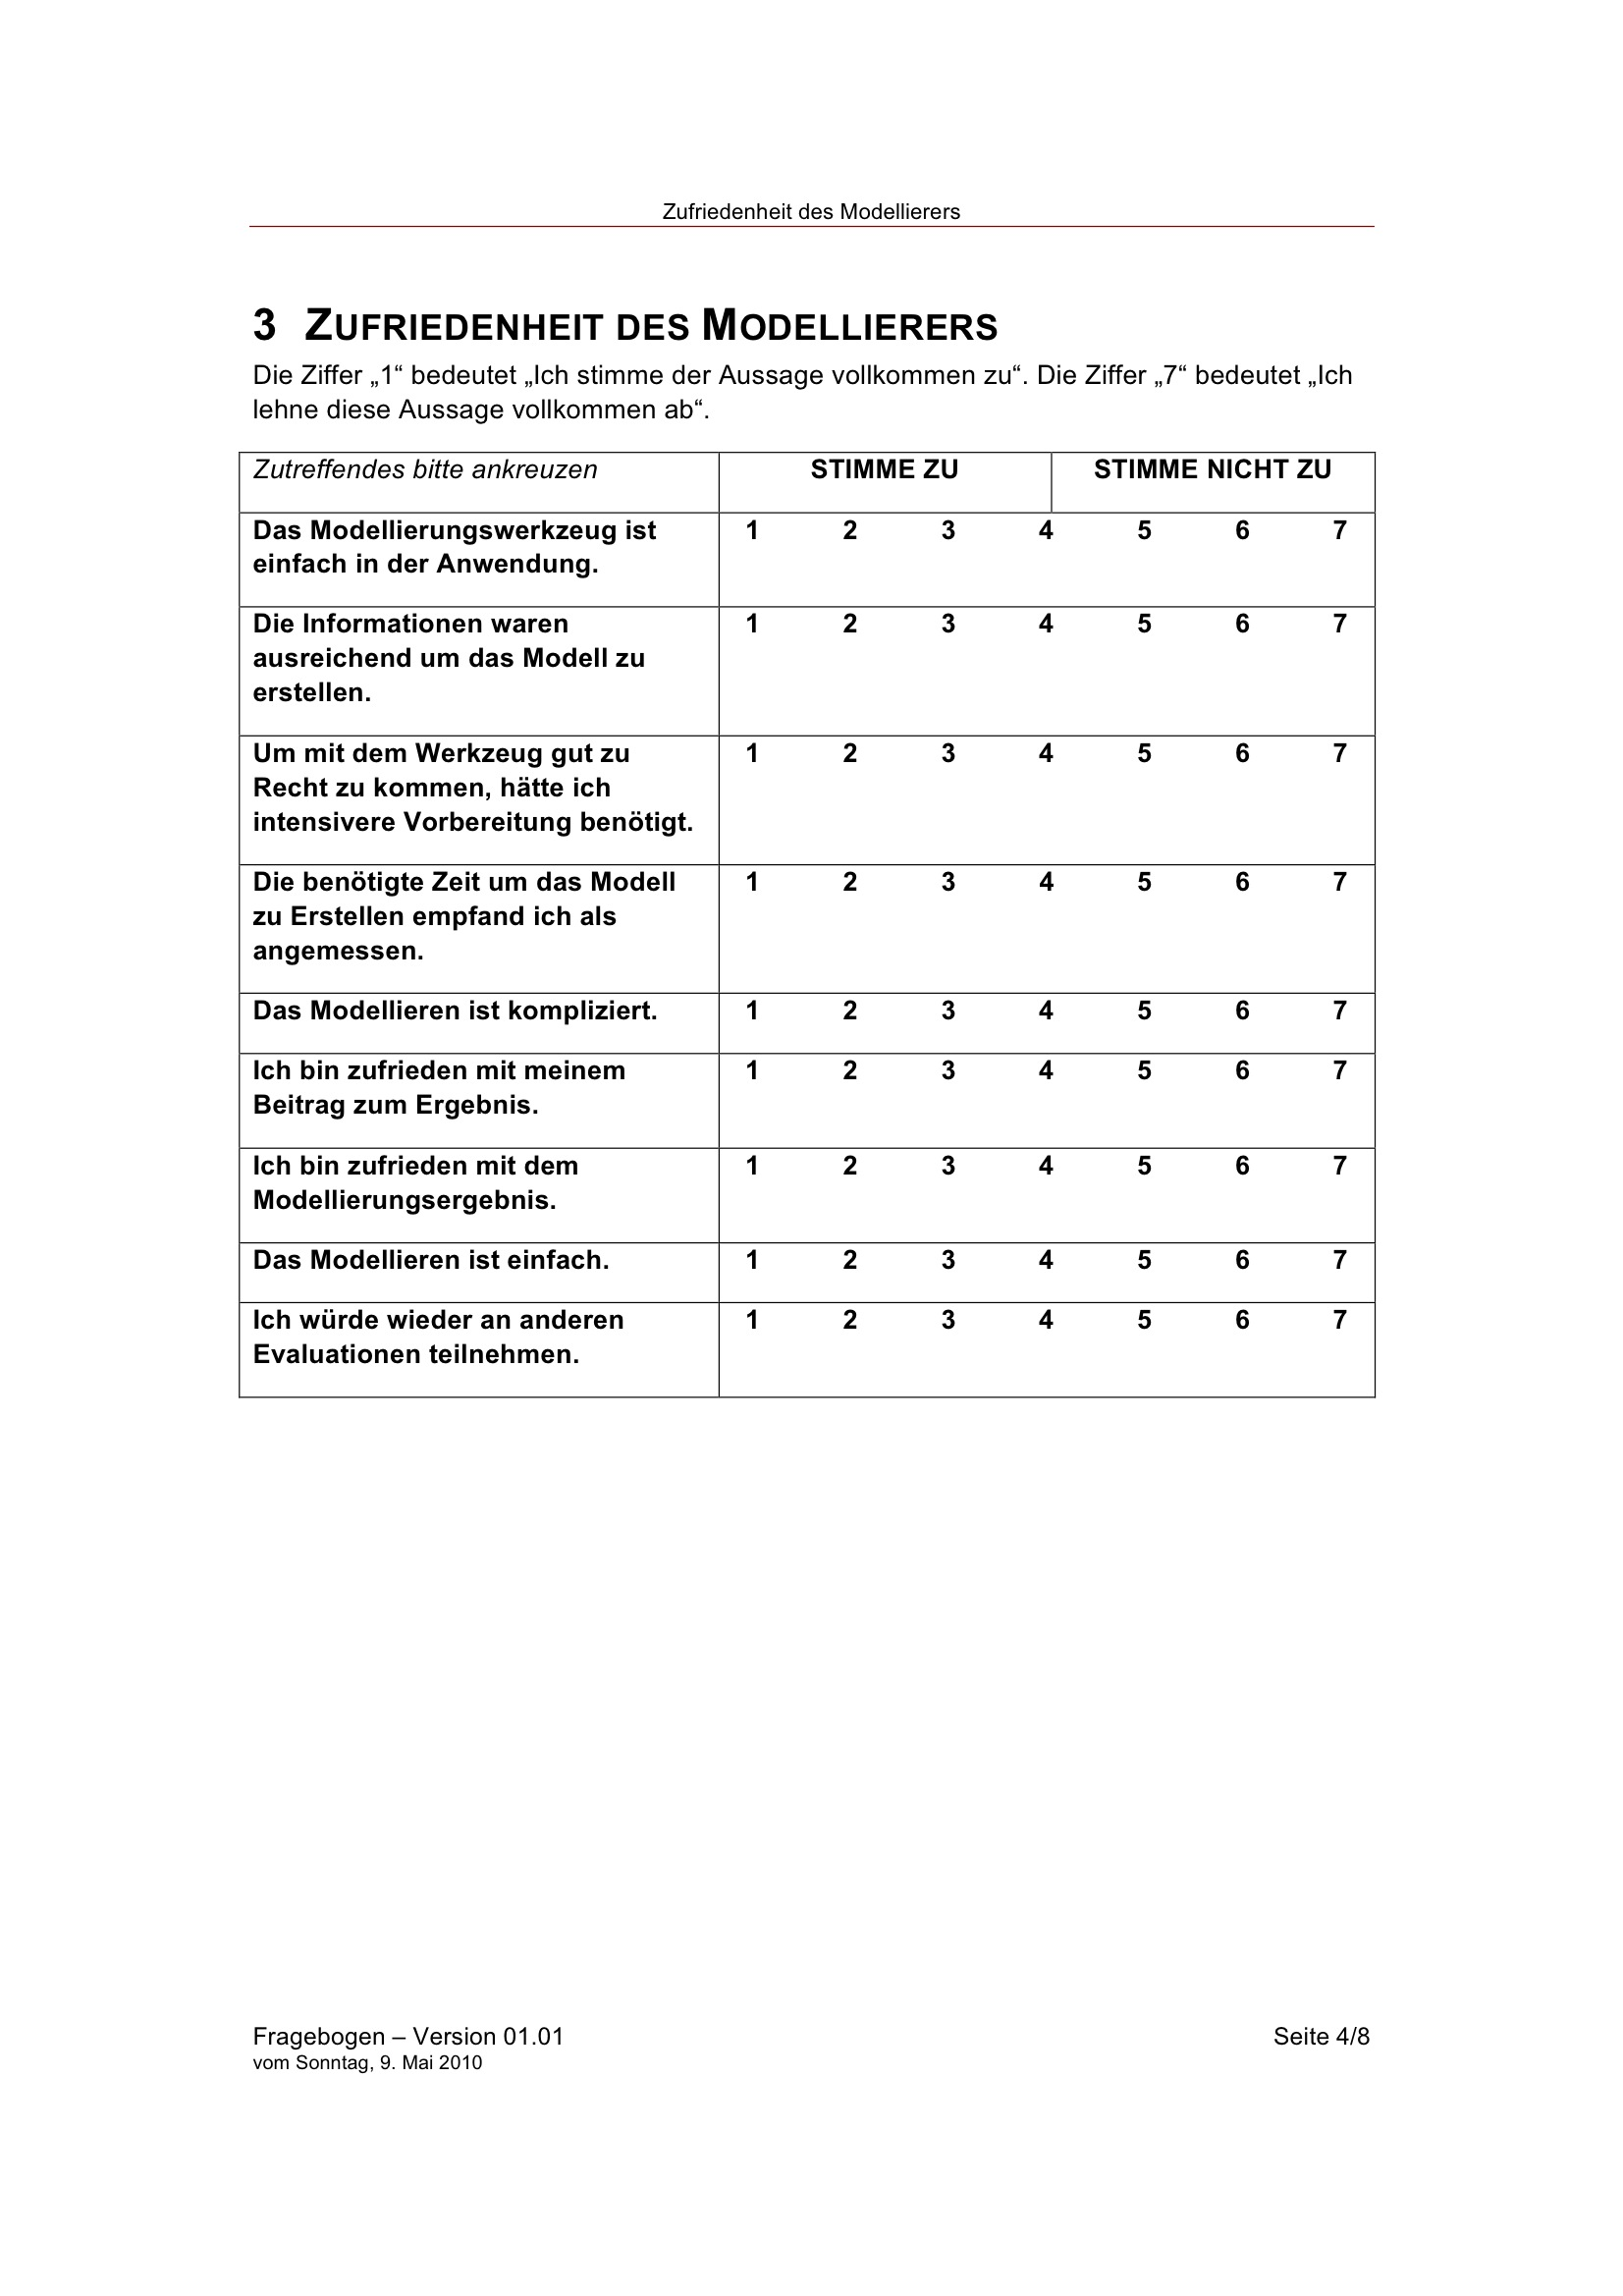
\includegraphics[width=0.9\textwidth]{img/AnhangEmpirie/fb4_2-04.jpeg}%
	}
	\caption{Zweiter Fragebogen für Evaluierungsblock 4 - Seite 4}
	\label{fig:img_AnhangEmpirie_fb4_2-04}
\end{figure}

\begin{figure}[htbp]
	\centering
	\fbox{%
		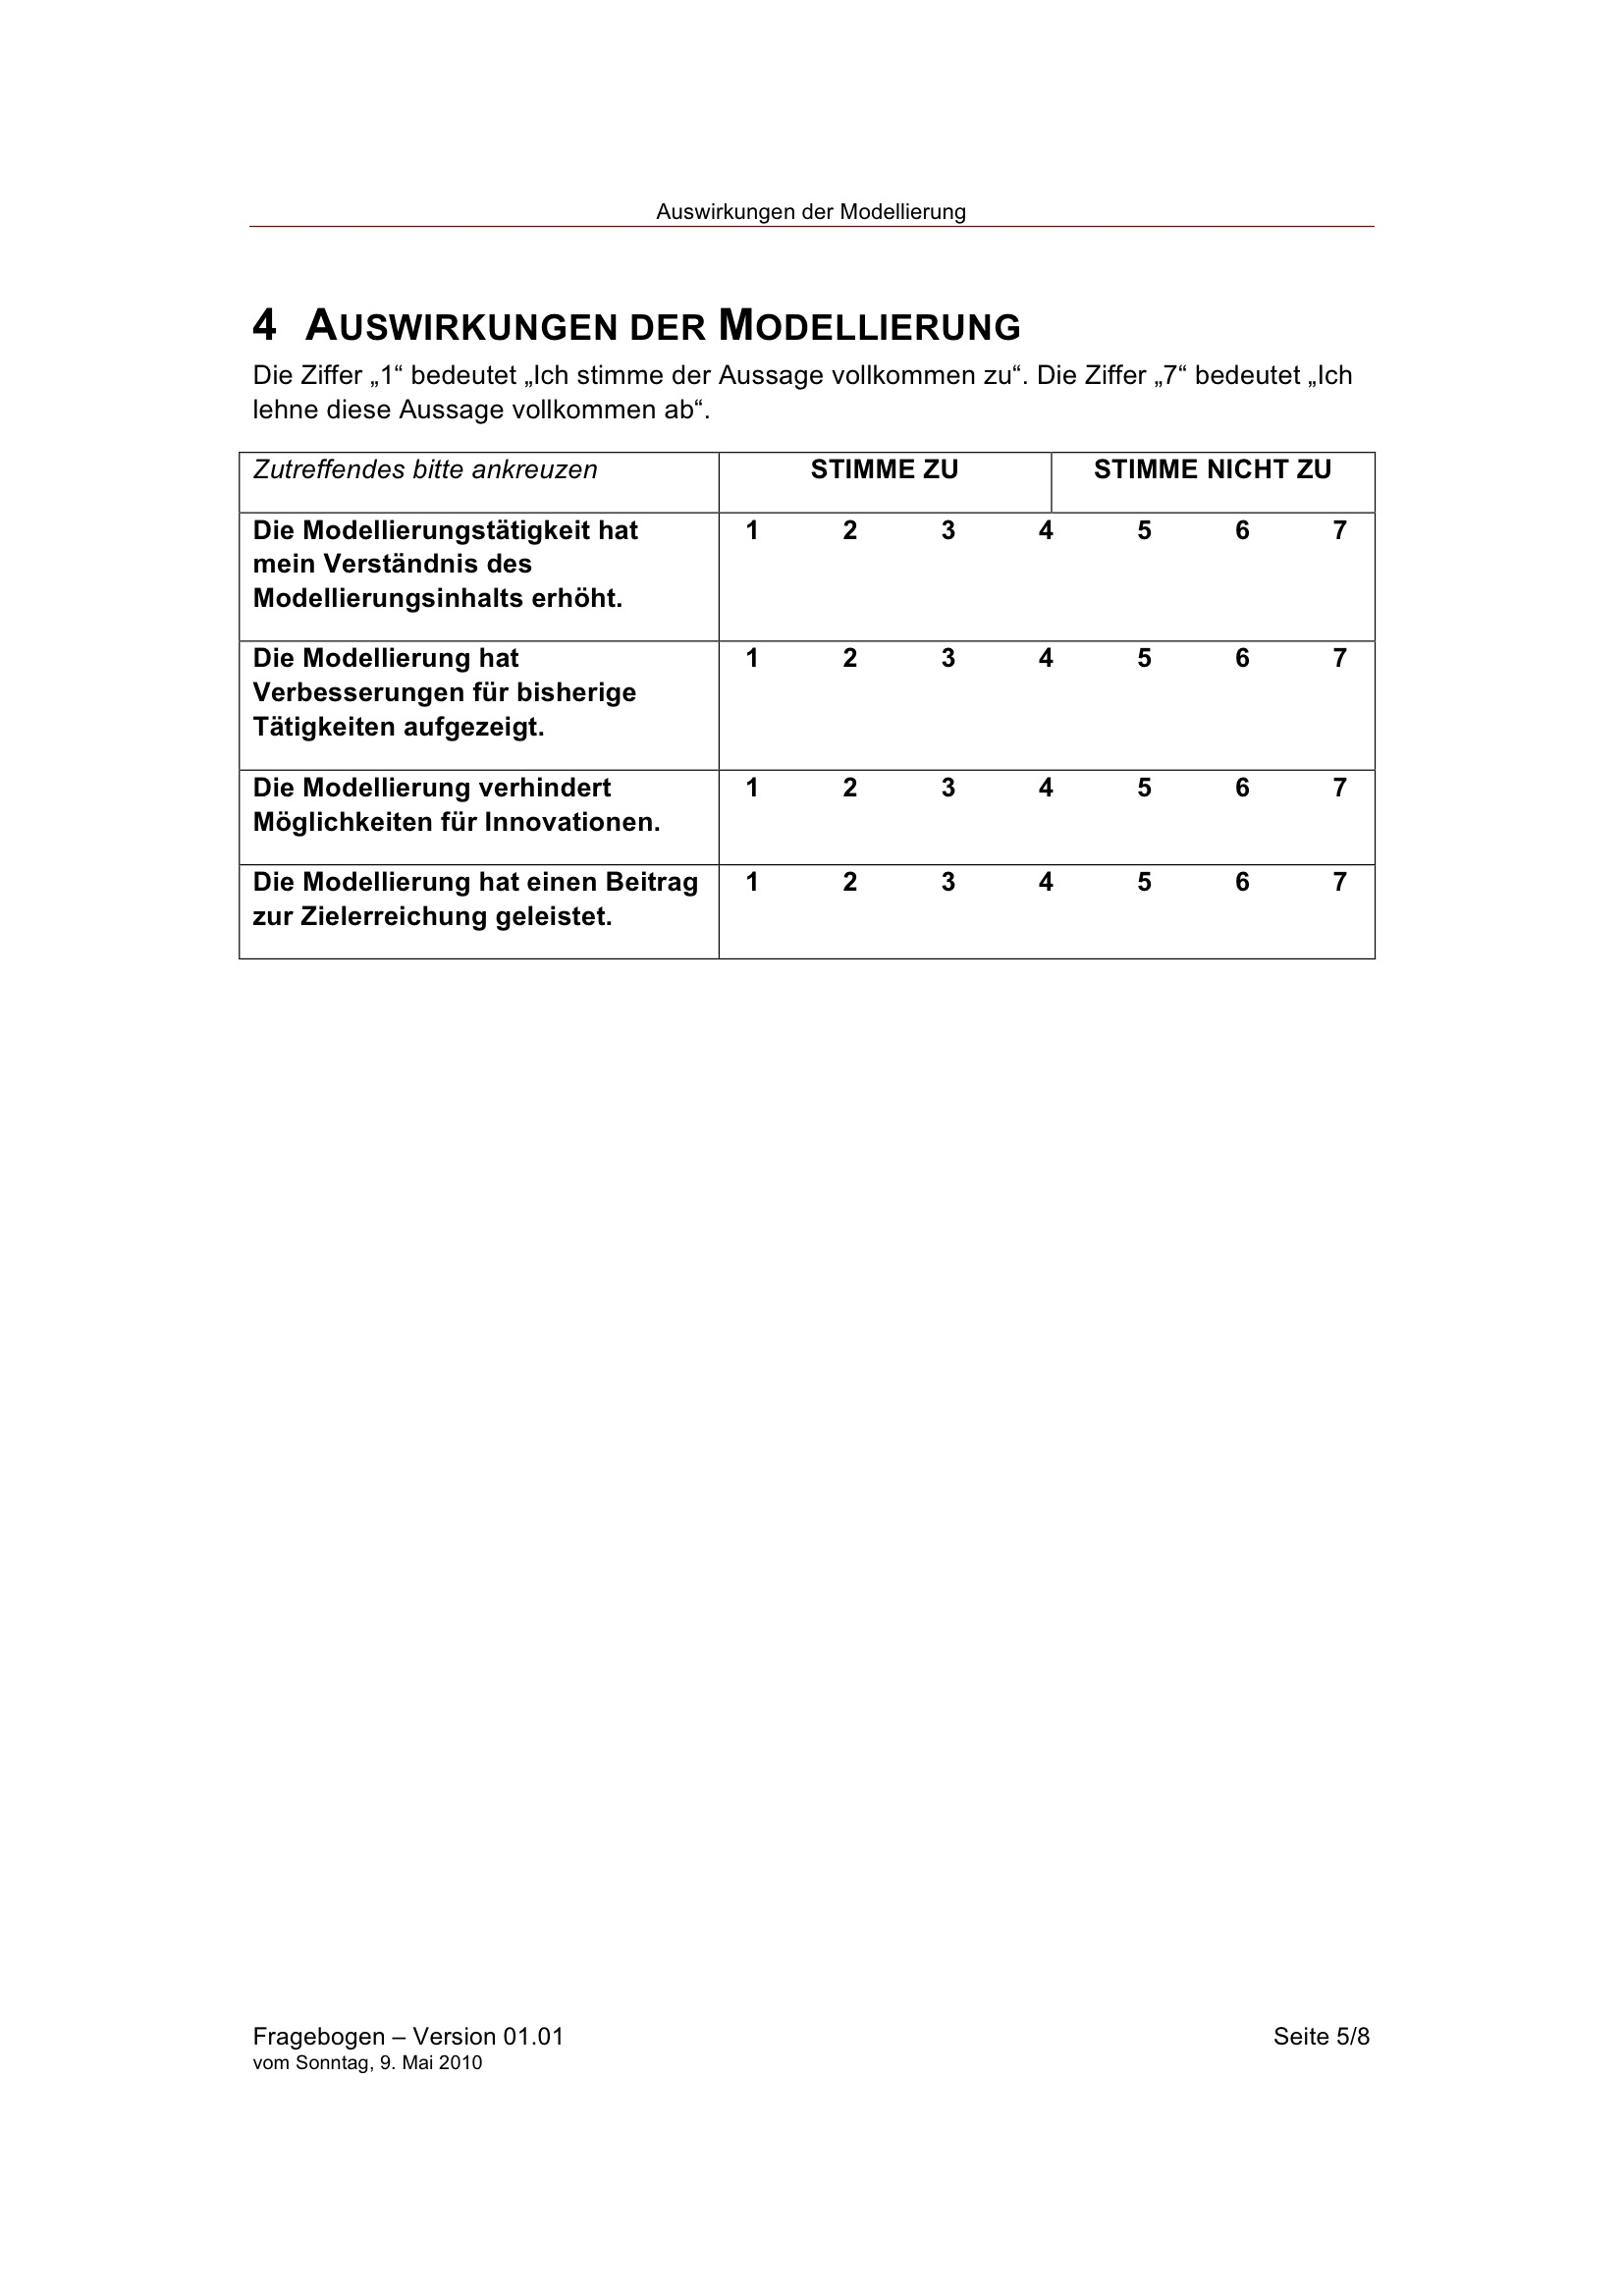
\includegraphics[width=0.9\textwidth]{img/AnhangEmpirie/fb4_2-05.jpeg}%
	}
	\caption{Zweiter Fragebogen für Evaluierungsblock 4 - Seite 5}
	\label{fig:img_AnhangEmpirie_fb4_2-05}
\end{figure}

\begin{figure}[htbp]
	\centering
	\fbox{%
		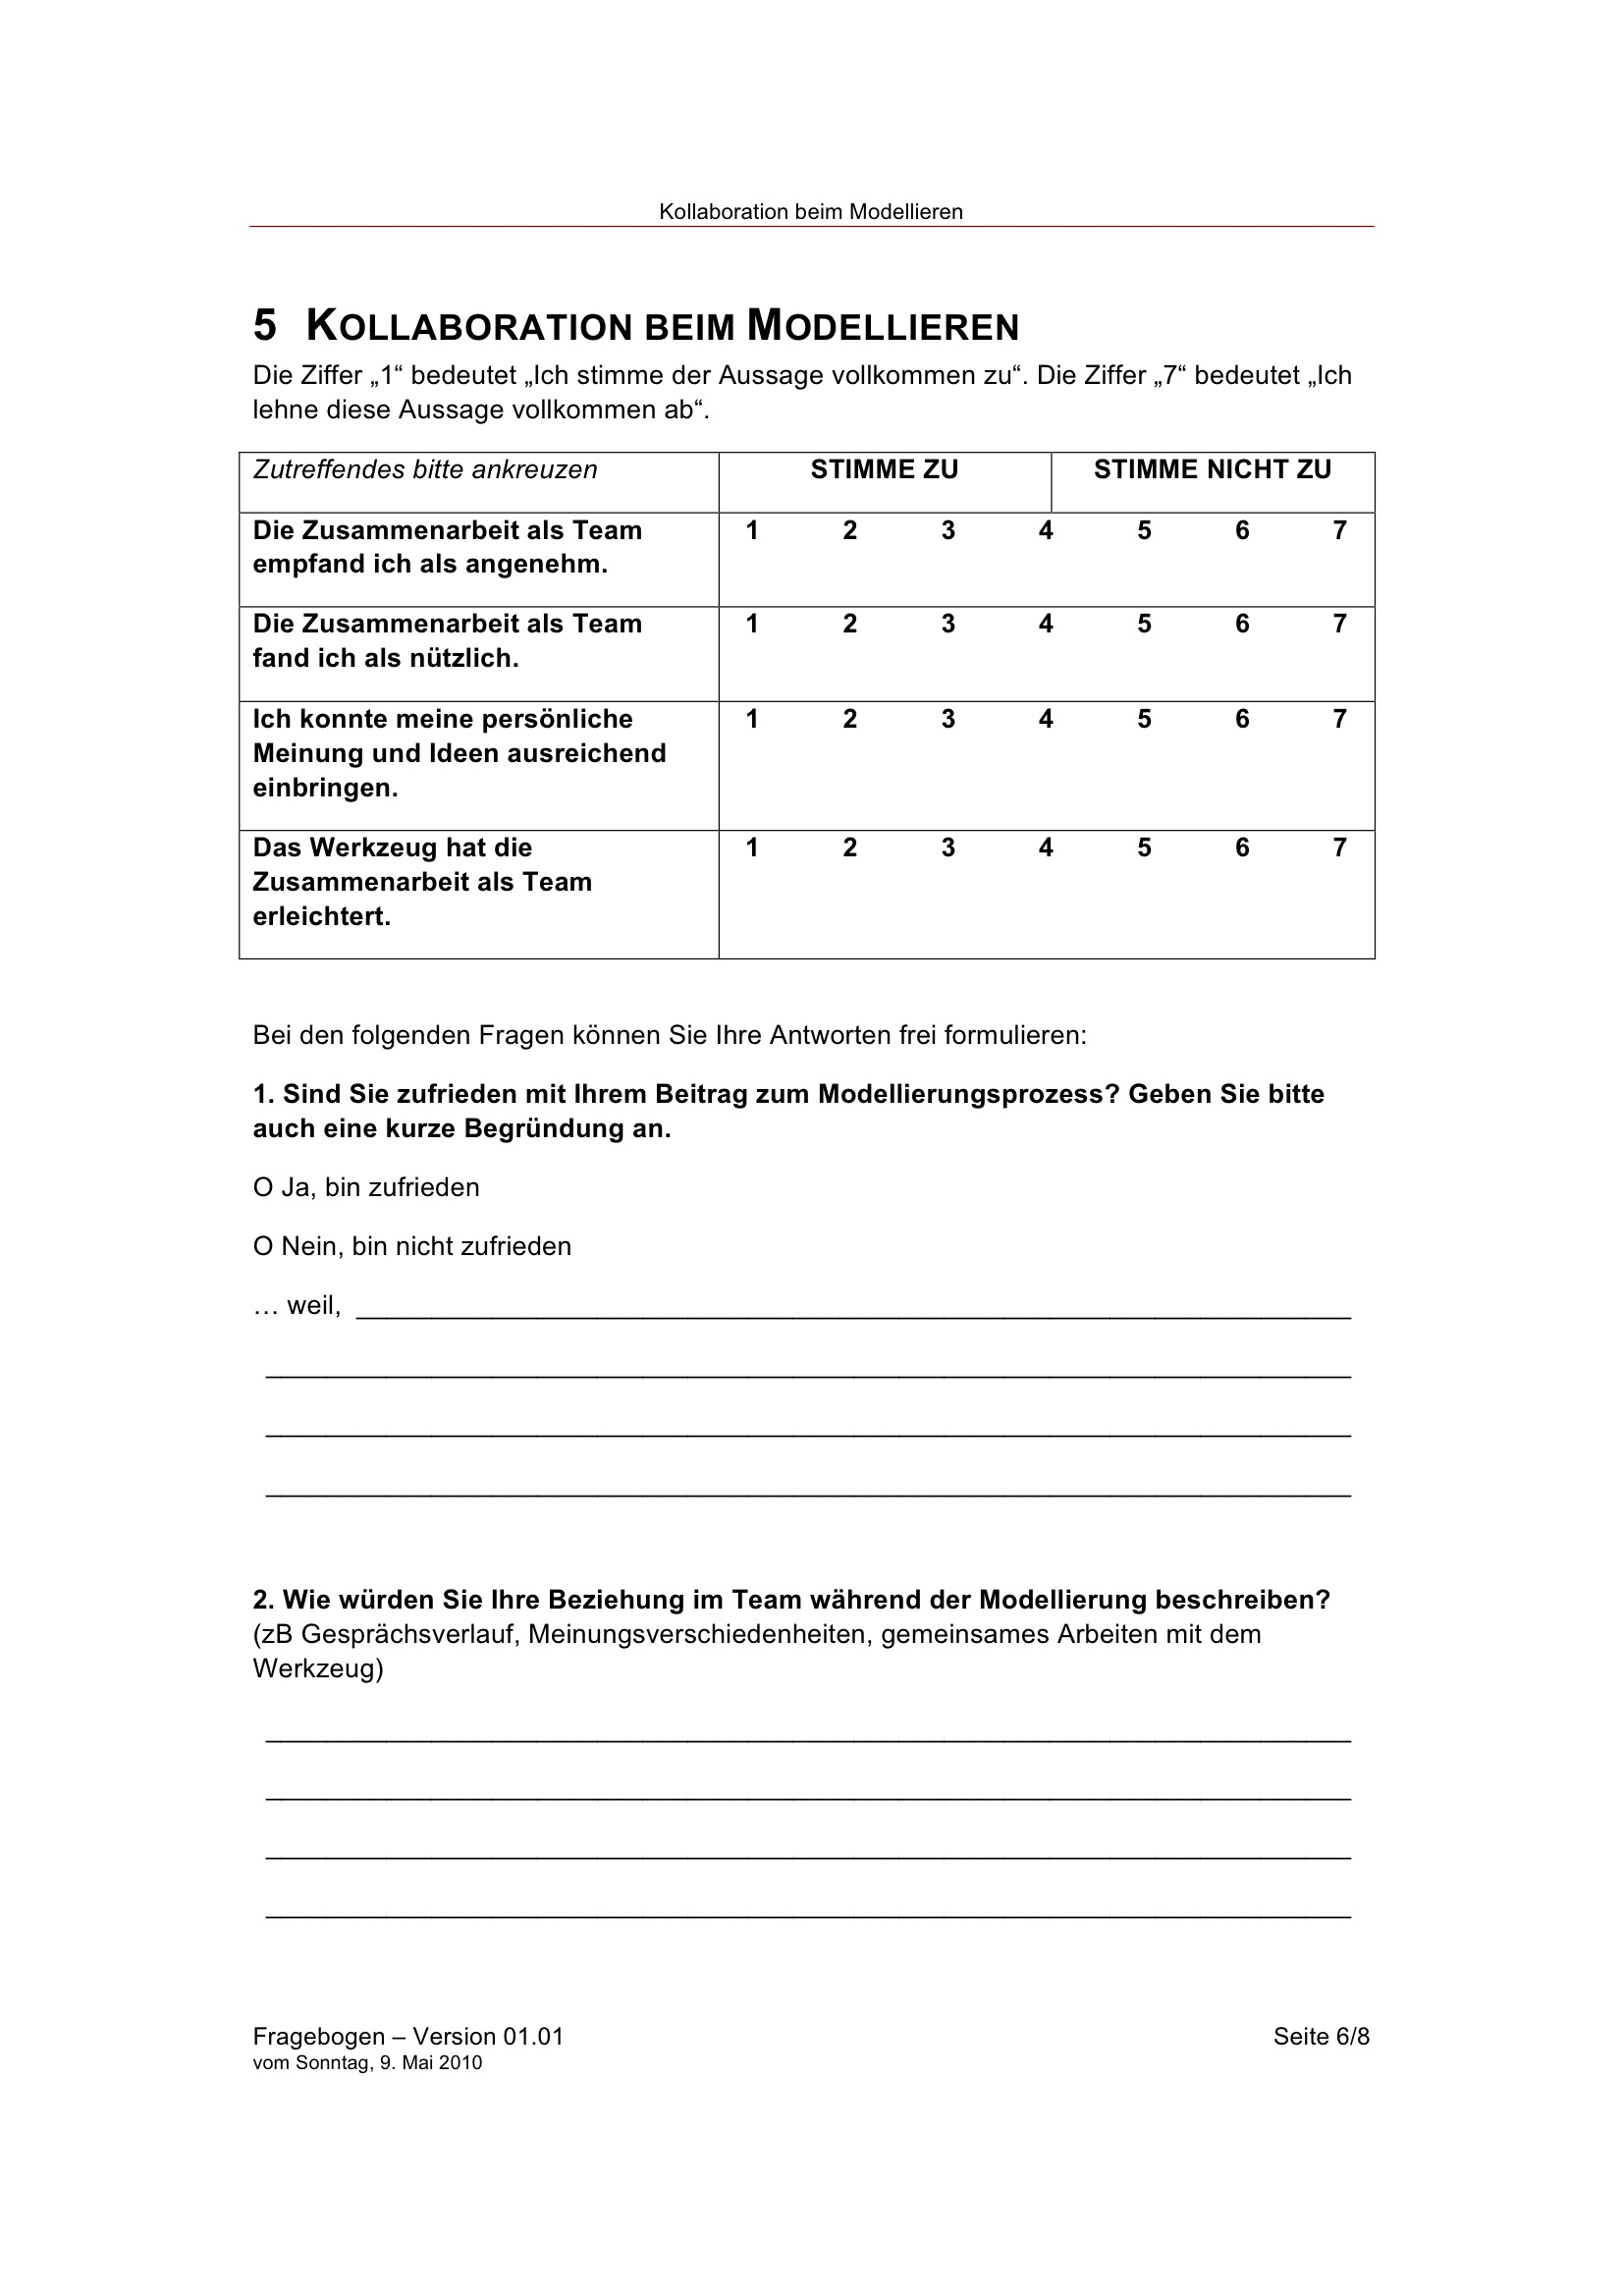
\includegraphics[width=0.9\textwidth]{img/AnhangEmpirie/fb4_2-06.jpeg}%
	}
	\caption{Zweiter Fragebogen für Evaluierungsblock 4 - Seite 6}
	\label{fig:img_AnhangEmpirie_fb4_2-06}
\end{figure}

\begin{figure}[htbp]
	\centering
	\fbox{%
		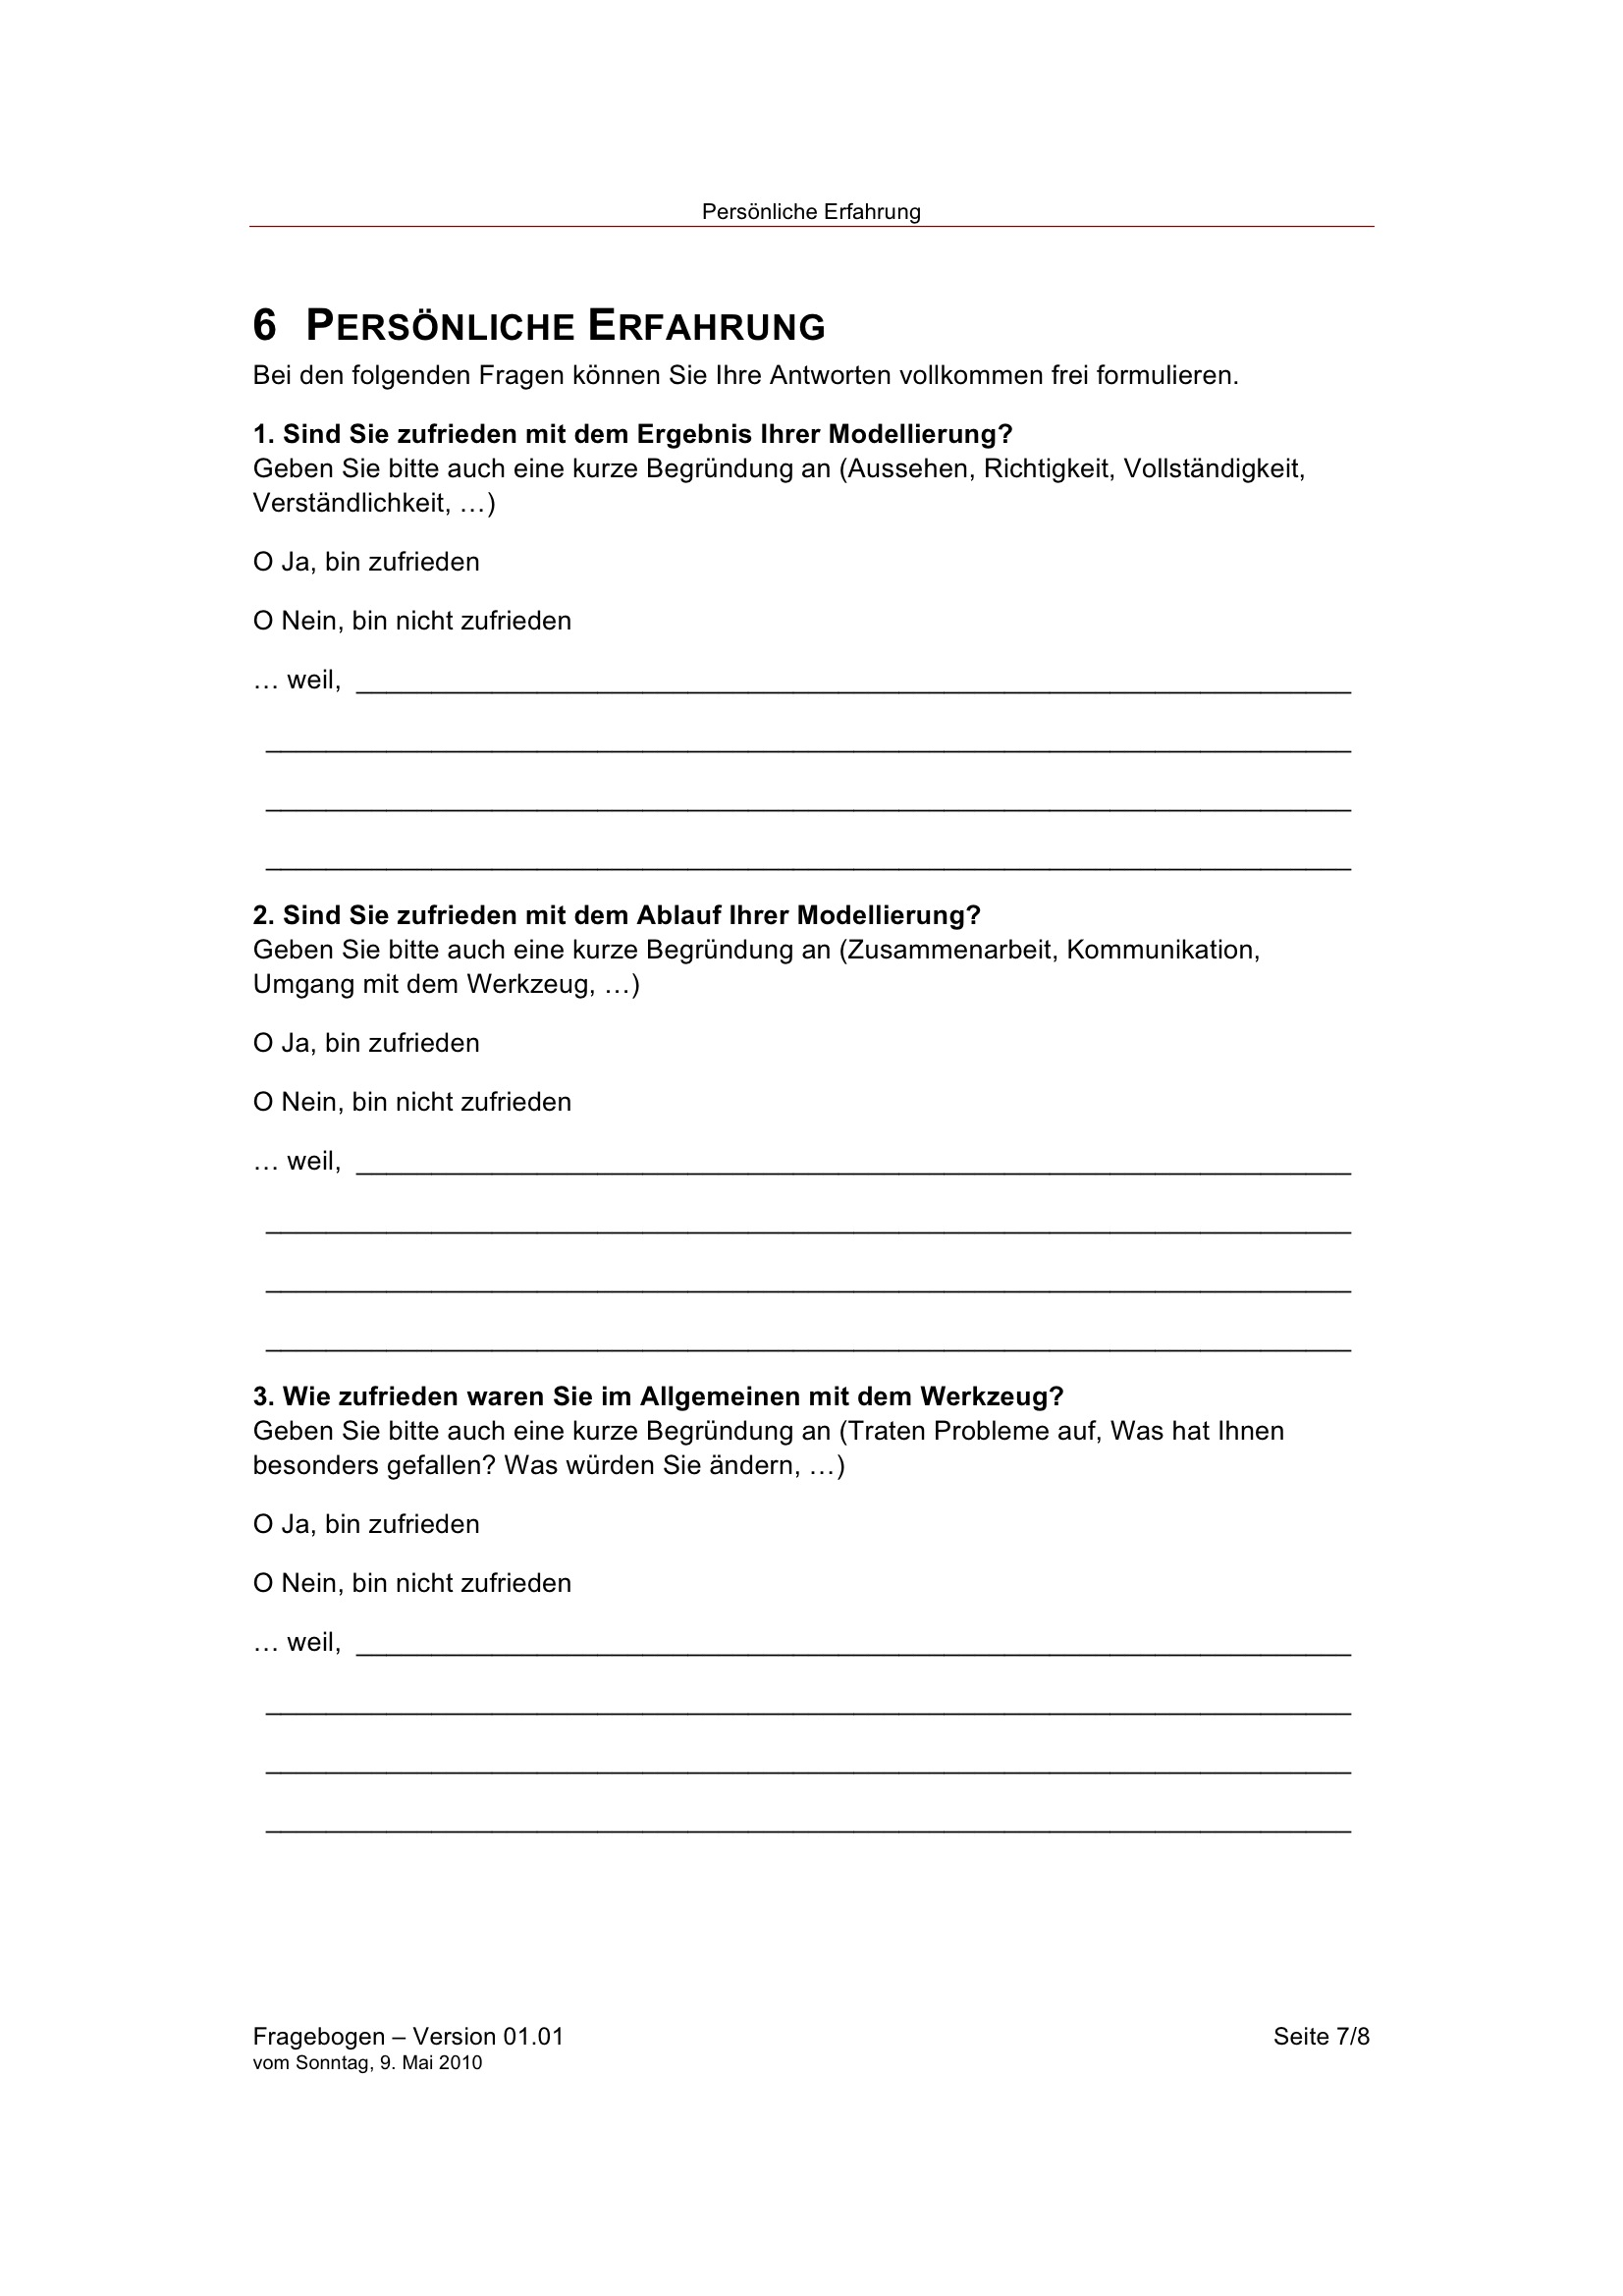
\includegraphics[width=0.9\textwidth]{img/AnhangEmpirie/fb4_2-07.jpeg}%
	}
	\caption{Zweiter Fragebogen für Evaluierungsblock 4 - Seite 7}
	\label{fig:img_AnhangEmpirie_fb4_2-07}
\end{figure}

\begin{figure}[htbp]
	\centering
	\fbox{%
		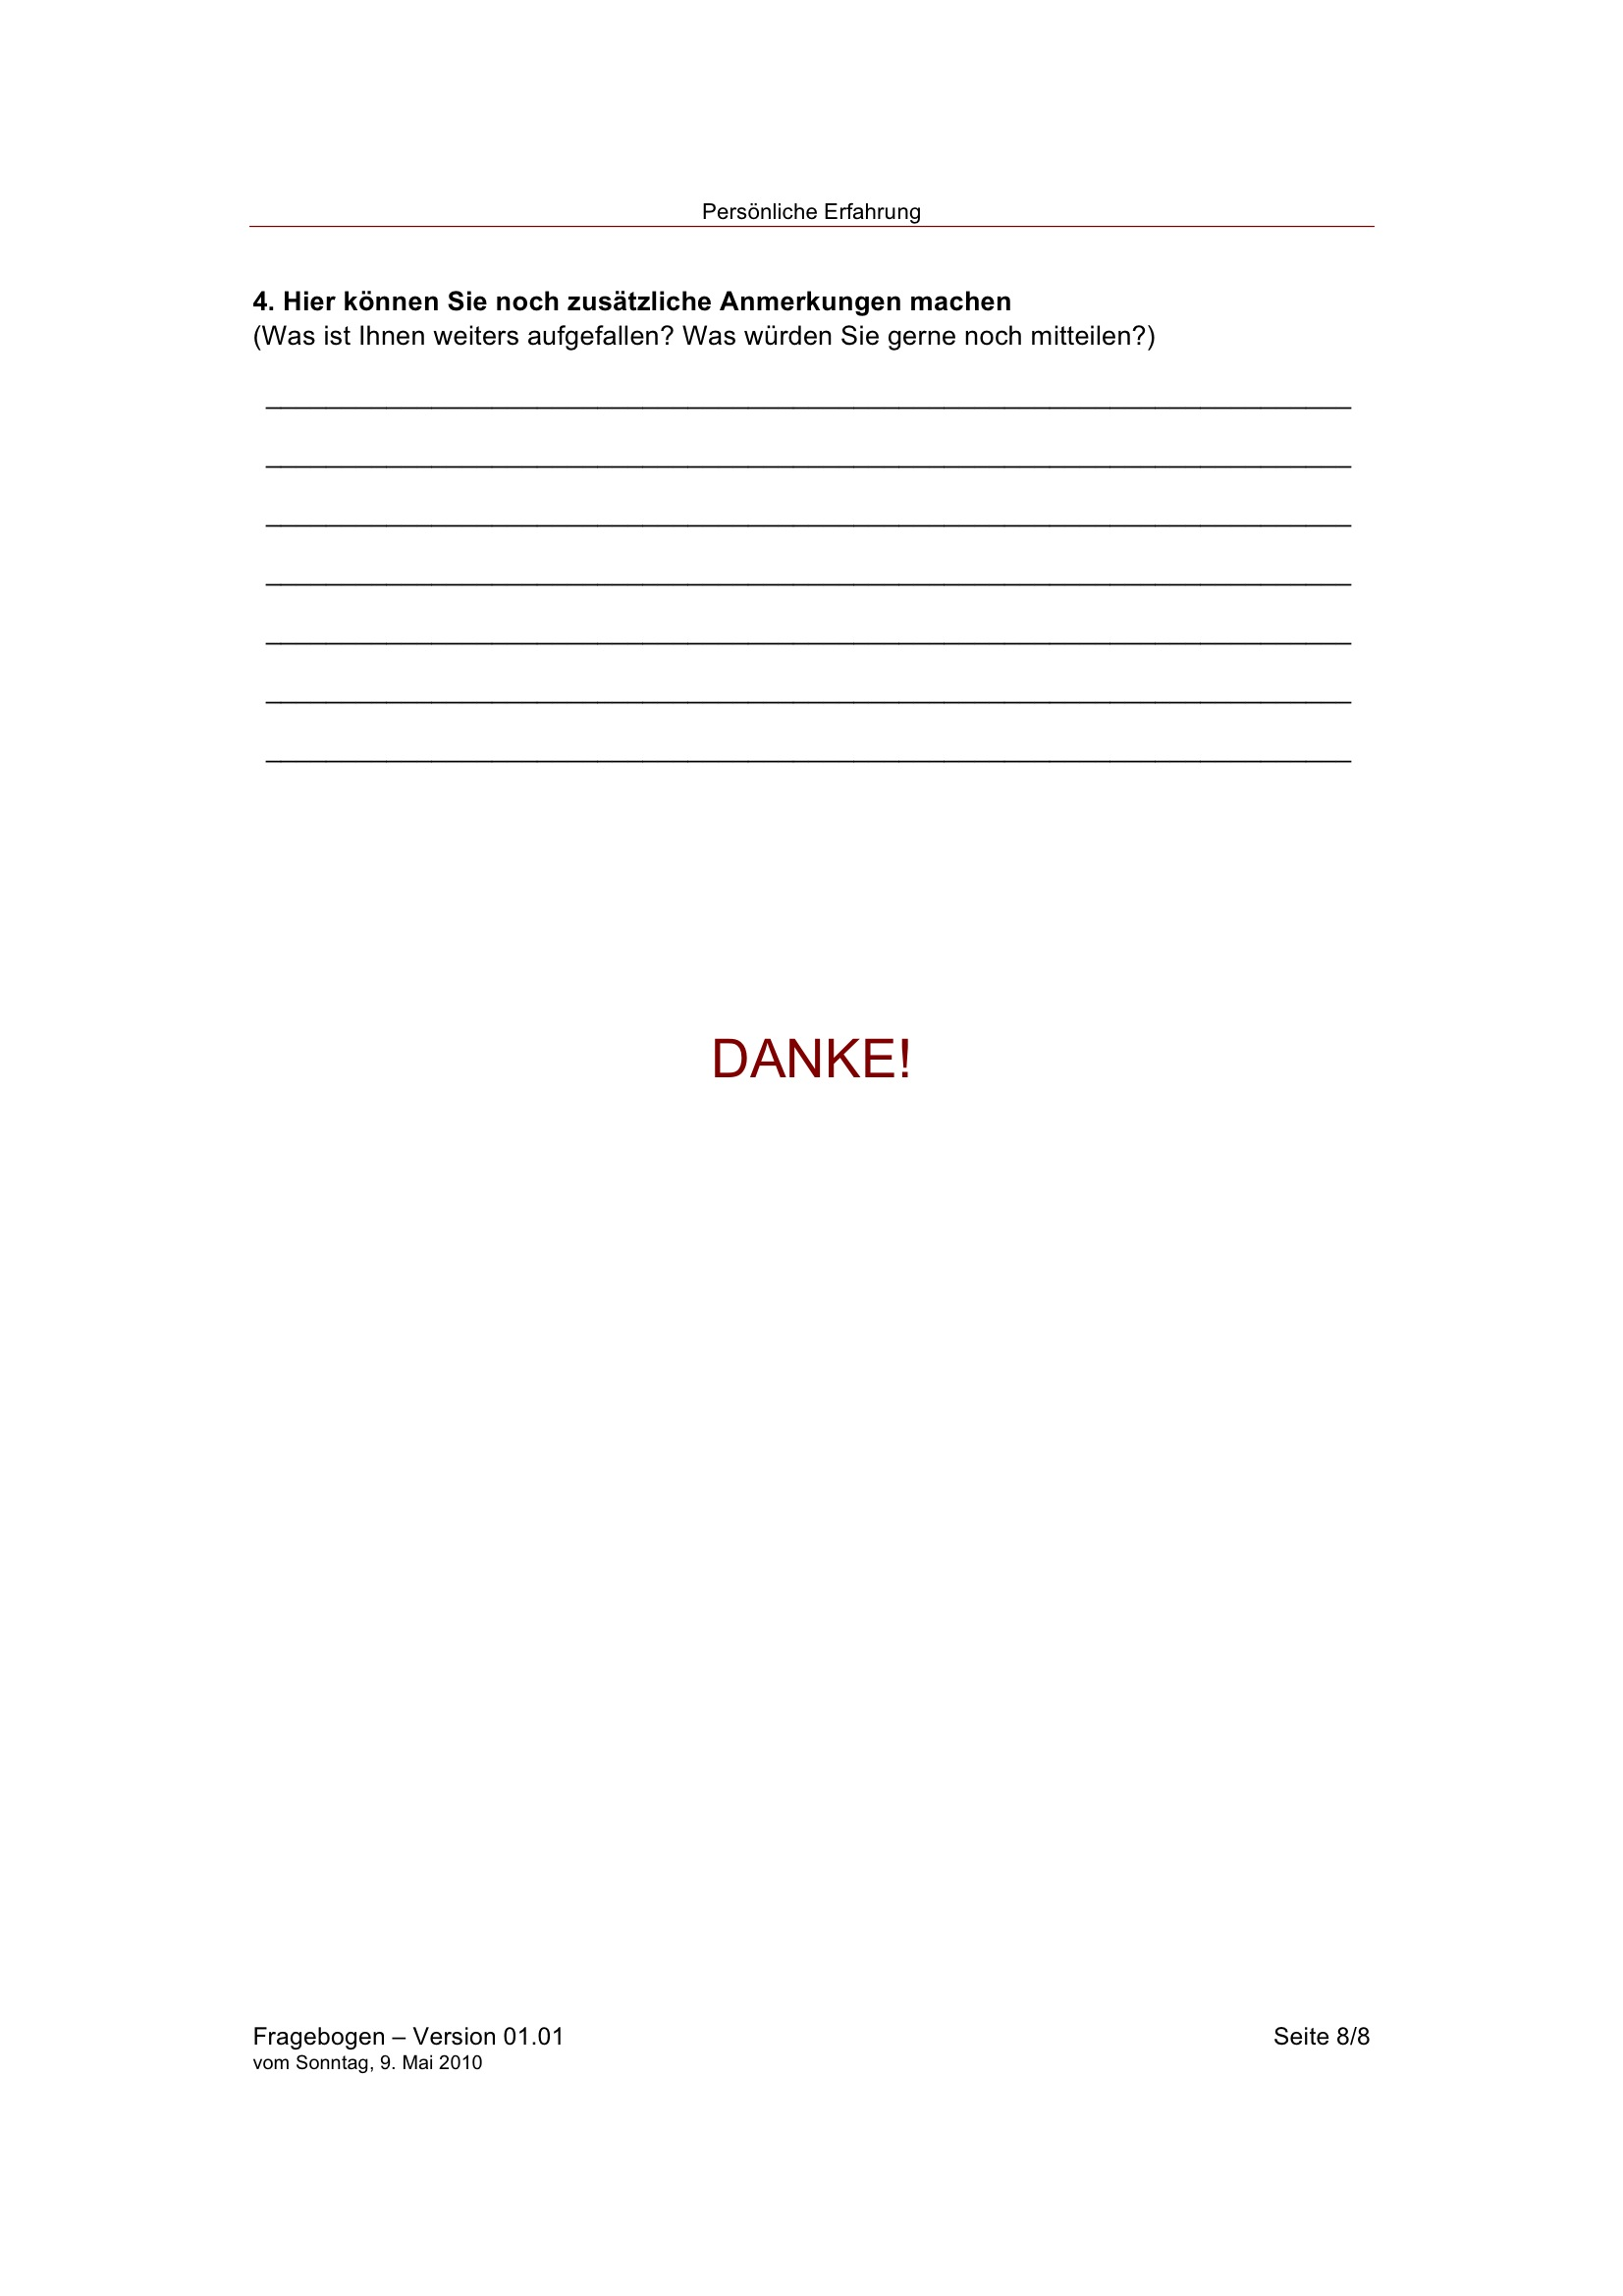
\includegraphics[width=0.9\textwidth]{img/AnhangEmpirie/fb4_2-08.jpeg}%
	}
	\caption{Zweiter Fragebogen für Evaluierungsblock 4 - Seite 8}
	\label{fig:img_AnhangEmpirie_fb4_2-08}
\end{figure}

\clearpage
\subsection{Frageböqgen aus Evaluierungsblock 5}
\label{sub:fb_eval5}

Die Abbildungen \ref{fig:img_AnhangEmpirie_fb5-01} bis \ref{fig:img_AnhangEmpirie_fb5-07} zeigen den in Evaluierungsblock 5 verwendeten Fragebogen. Der Aufbau des Fragebogens wurde von \citet{Bindreiter10} detailliert beschrieben und begründet.

\begin{figure}[htbp]
	\centering
	\fbox{%
		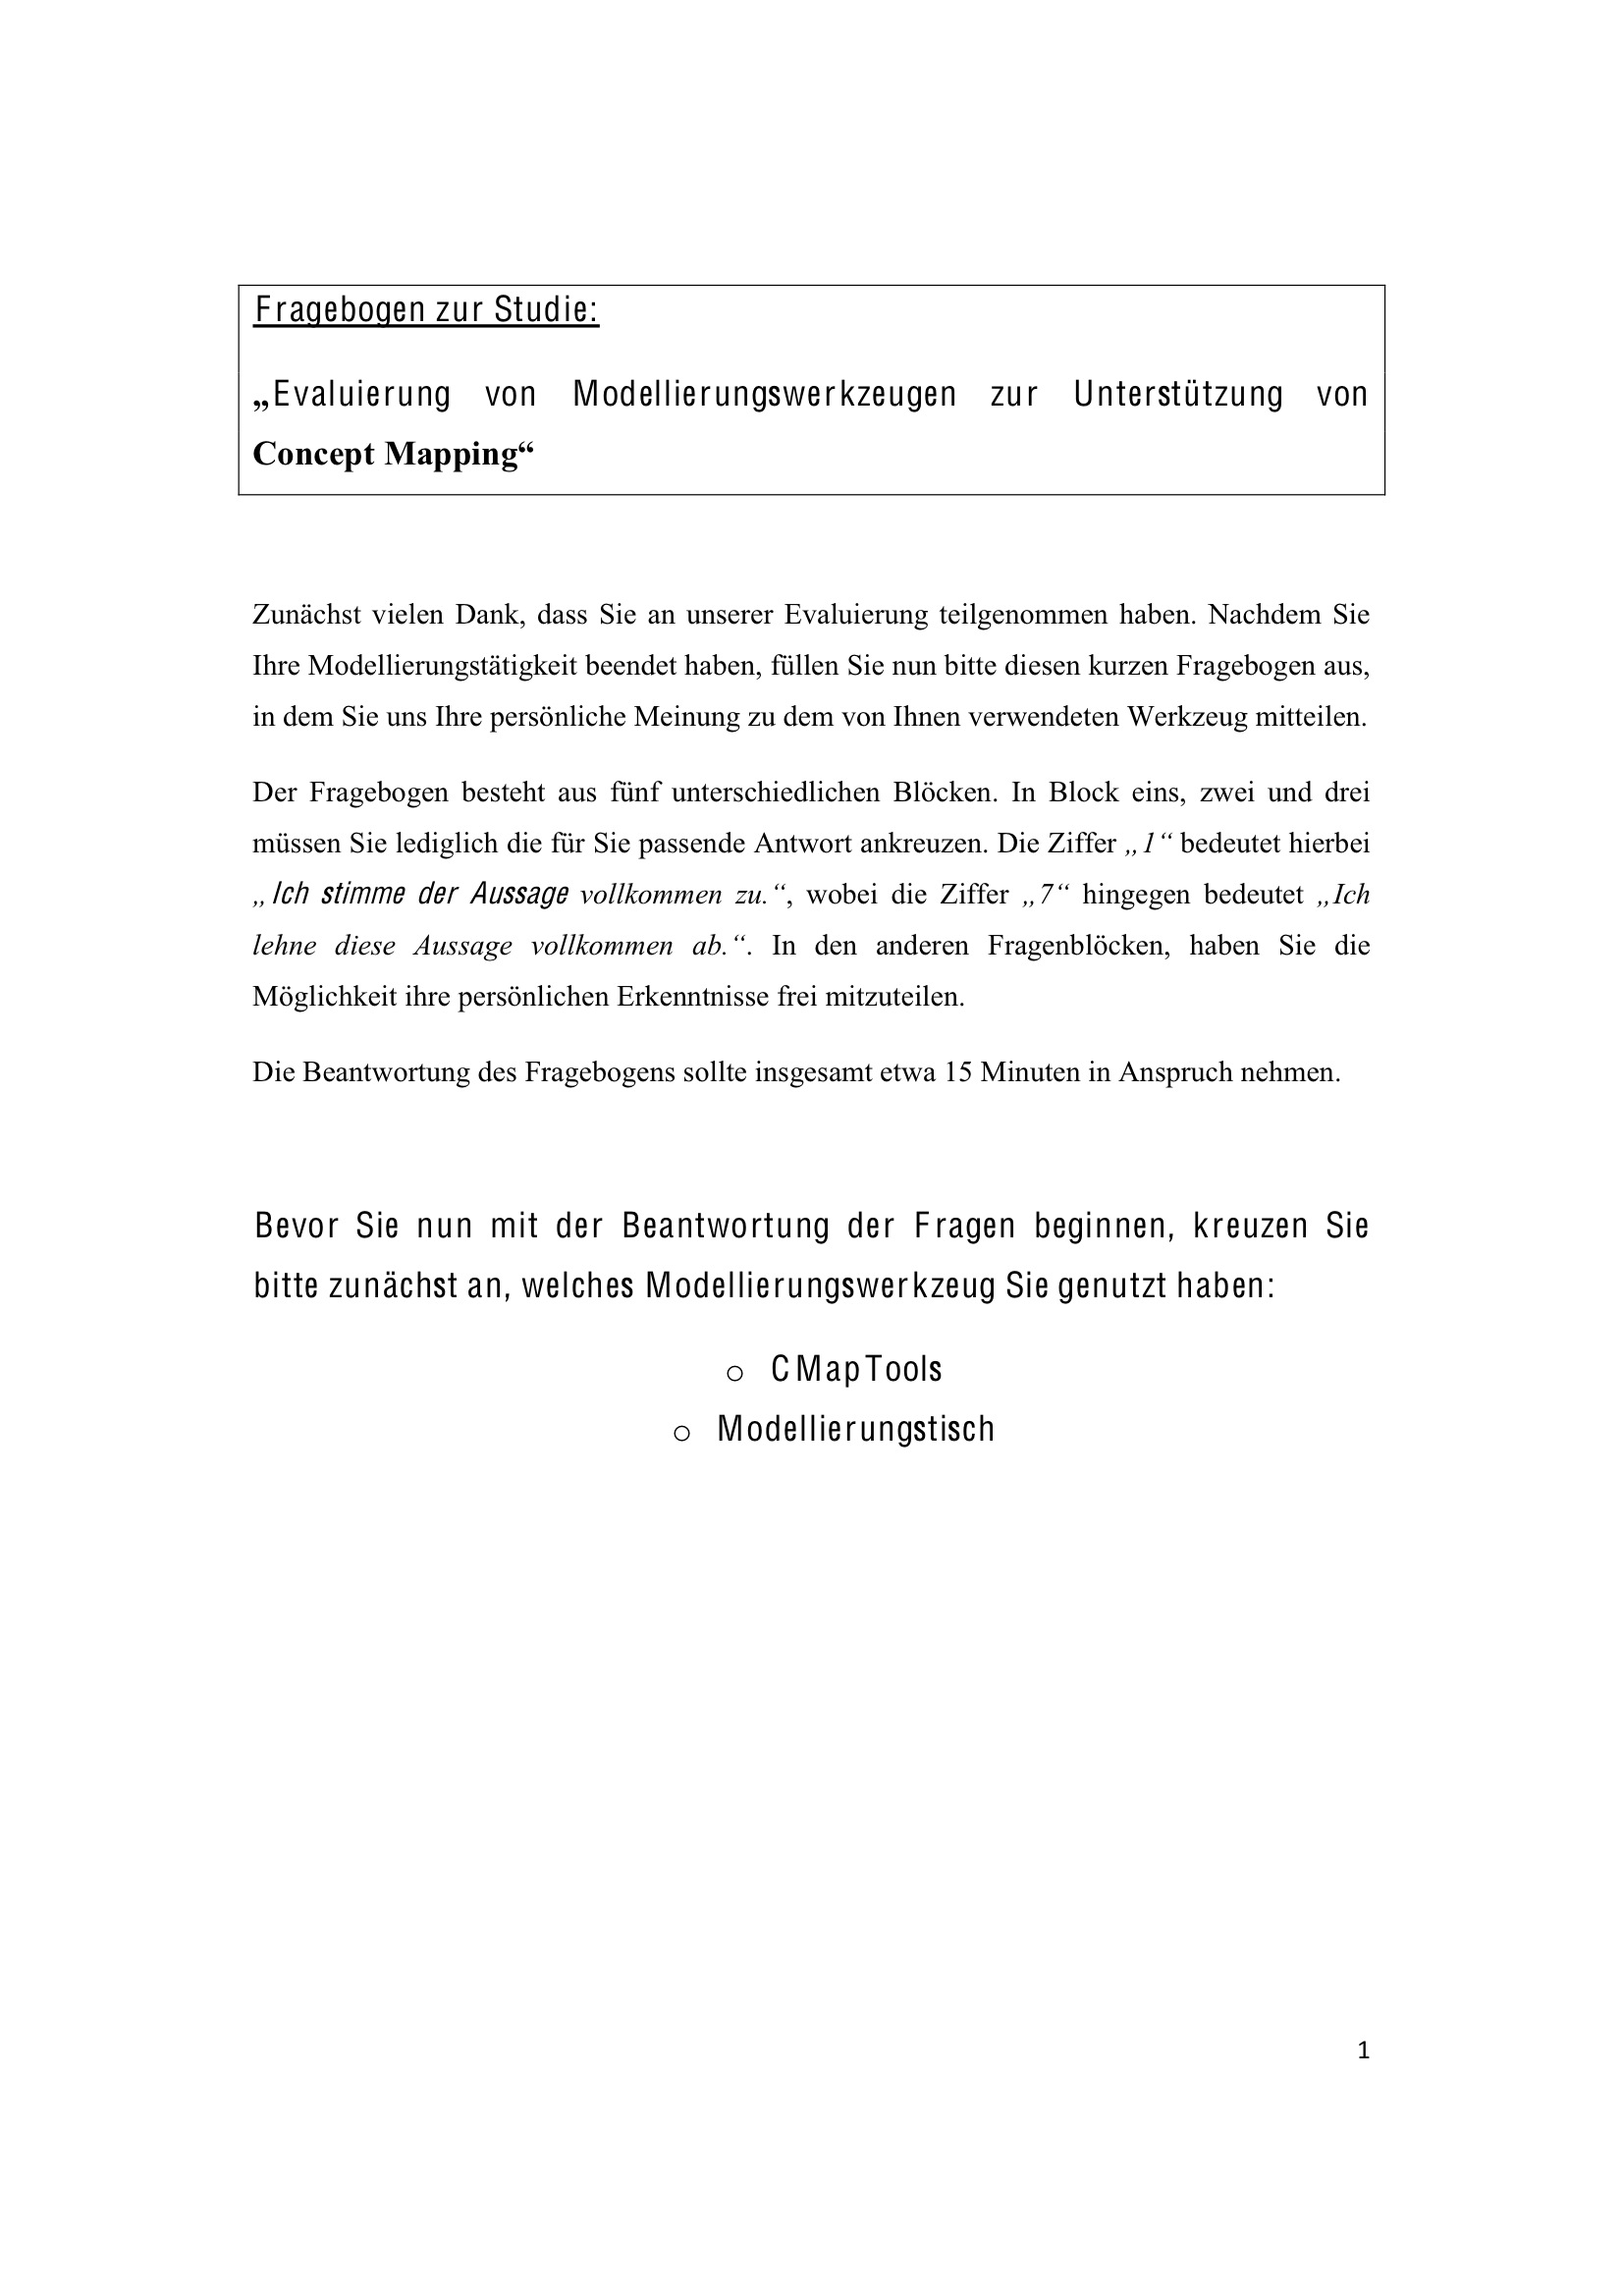
\includegraphics[width=0.9\textwidth]{img/AnhangEmpirie/fb5-01.jpeg}%
	}
	\caption{Fragebogen für Evaluierungsblock 5 - Seite 1}
	\label{fig:img_AnhangEmpirie_fb5-01}
\end{figure}

\begin{figure}[htbp]
	\centering
	\fbox{%
		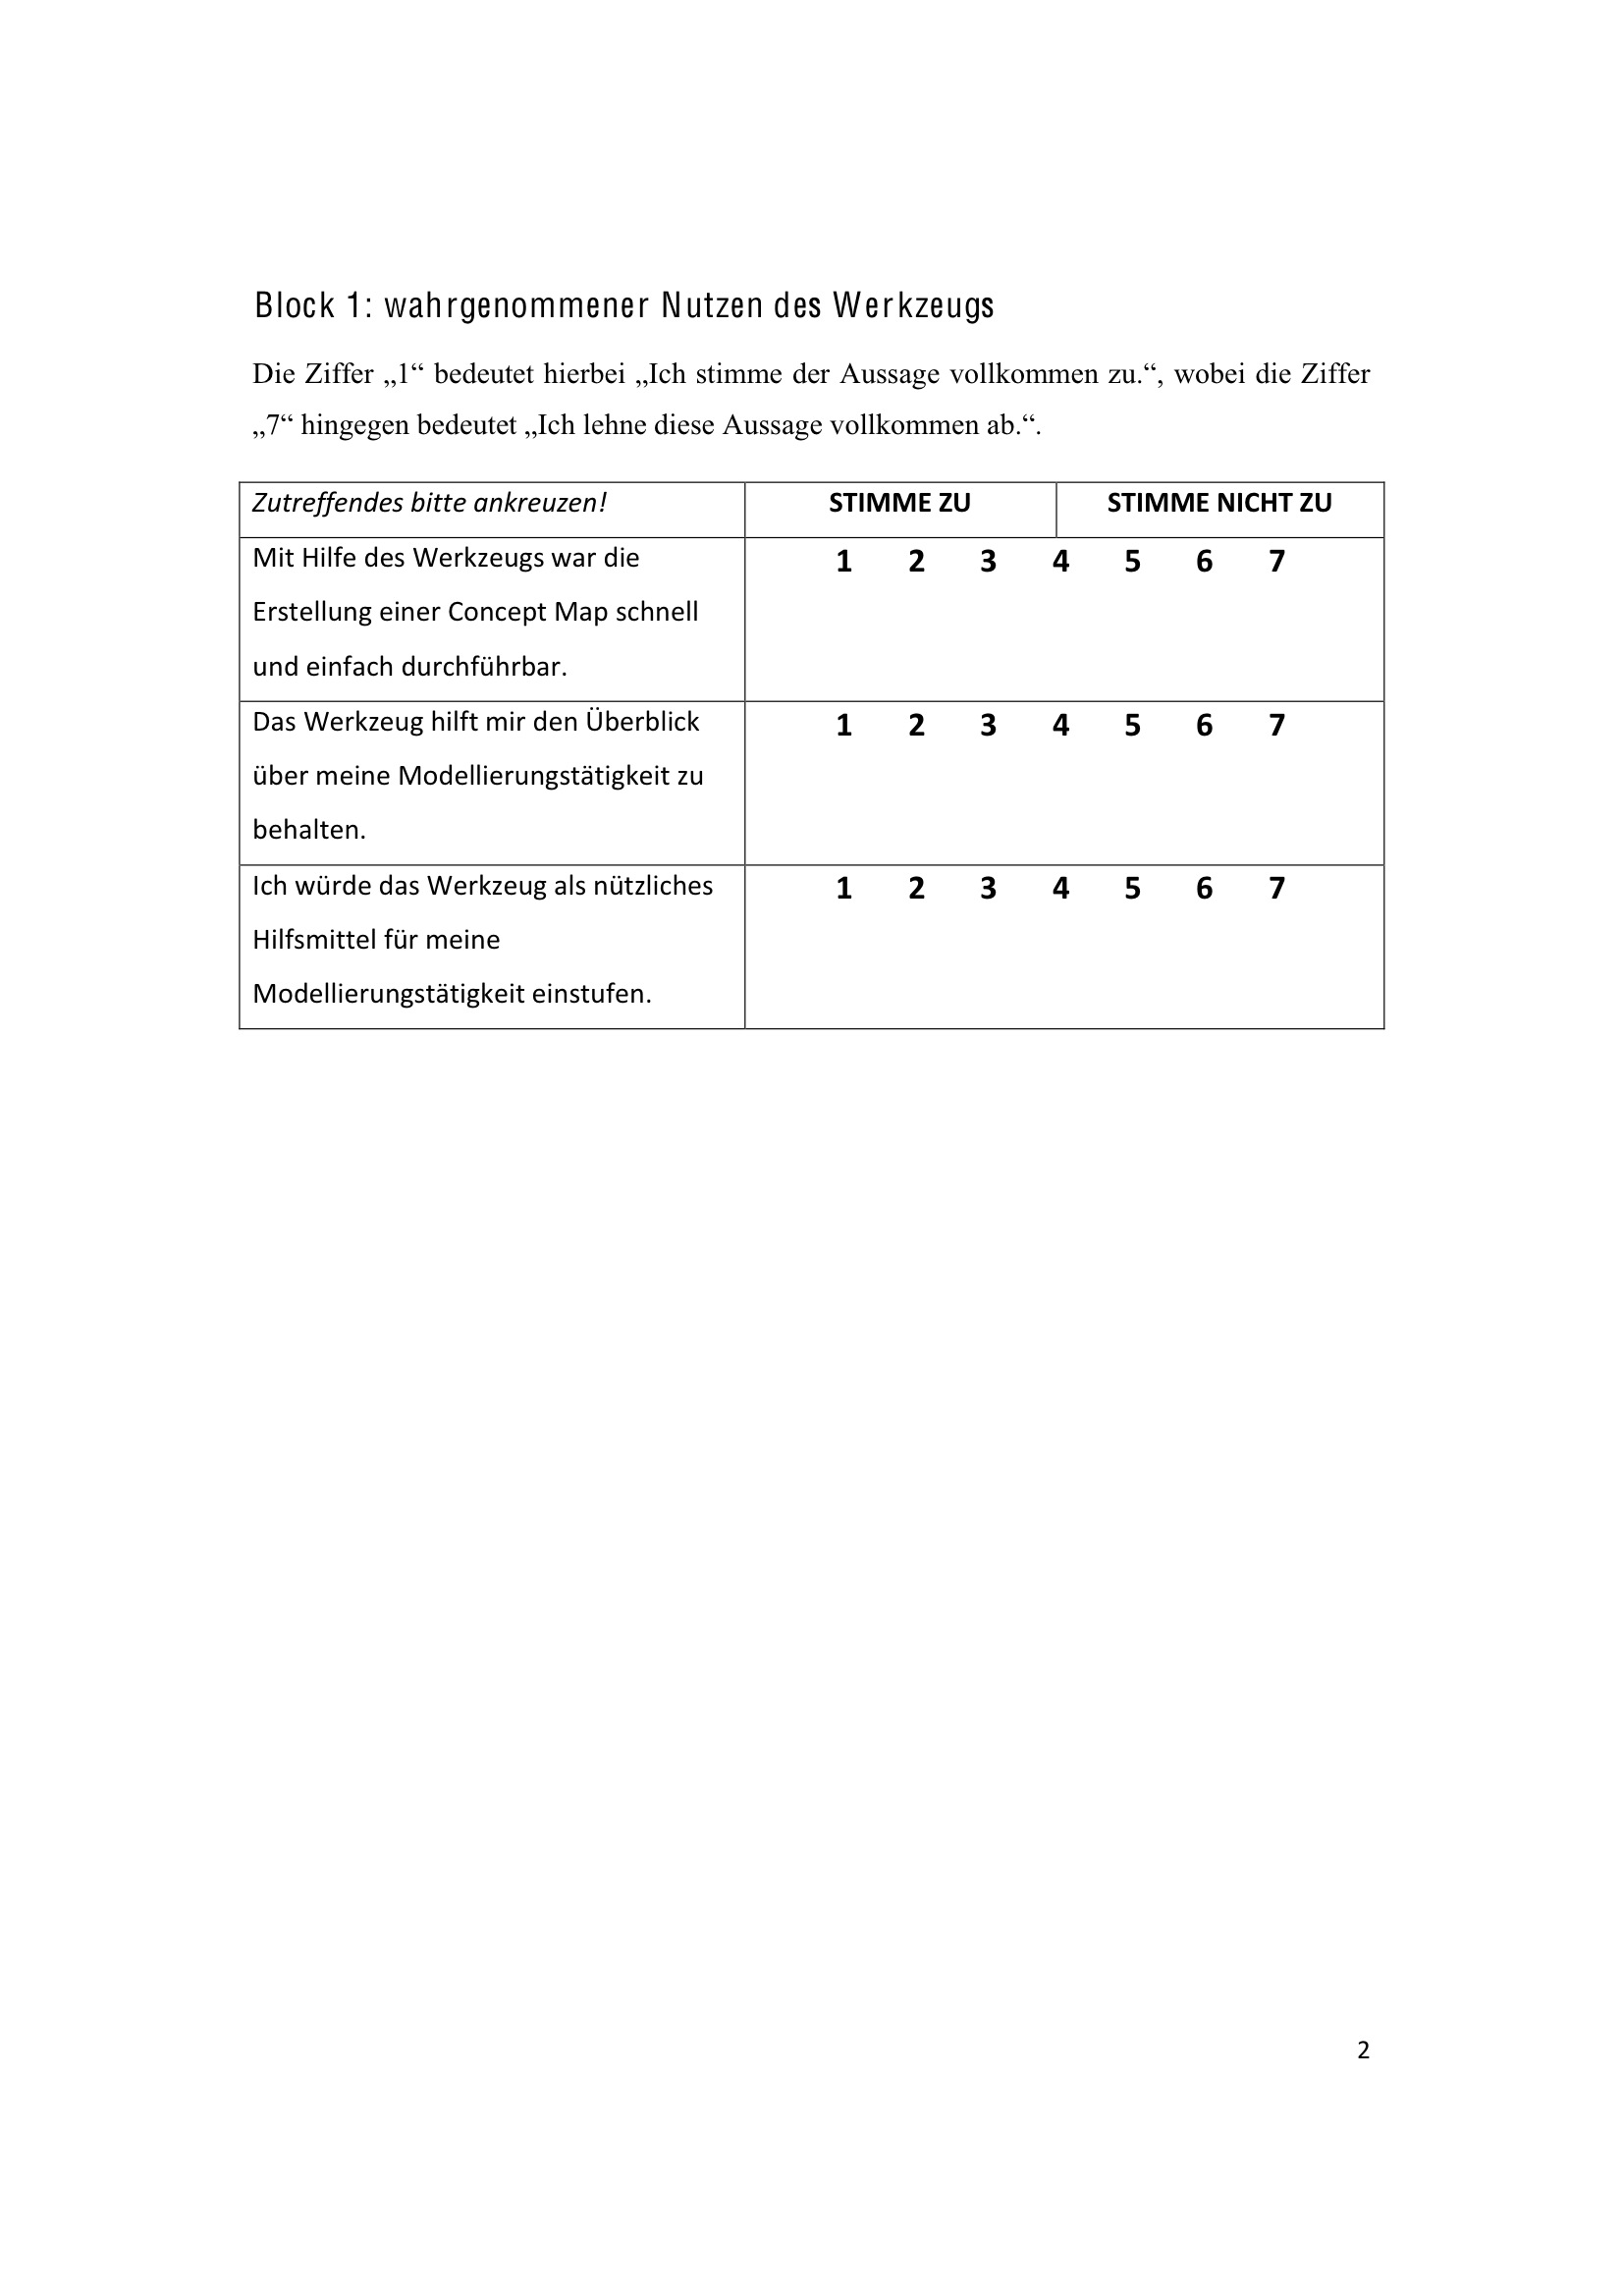
\includegraphics[width=0.9\textwidth]{img/AnhangEmpirie/fb5-02.jpeg}%
	}
	\caption{Fragebogen für Evaluierungsblock 5 - Seite 2}
	\label{fig:img_AnhangEmpirie_fb5-02}
\end{figure}

\begin{figure}[htbp]
	\centering
	\fbox{%
		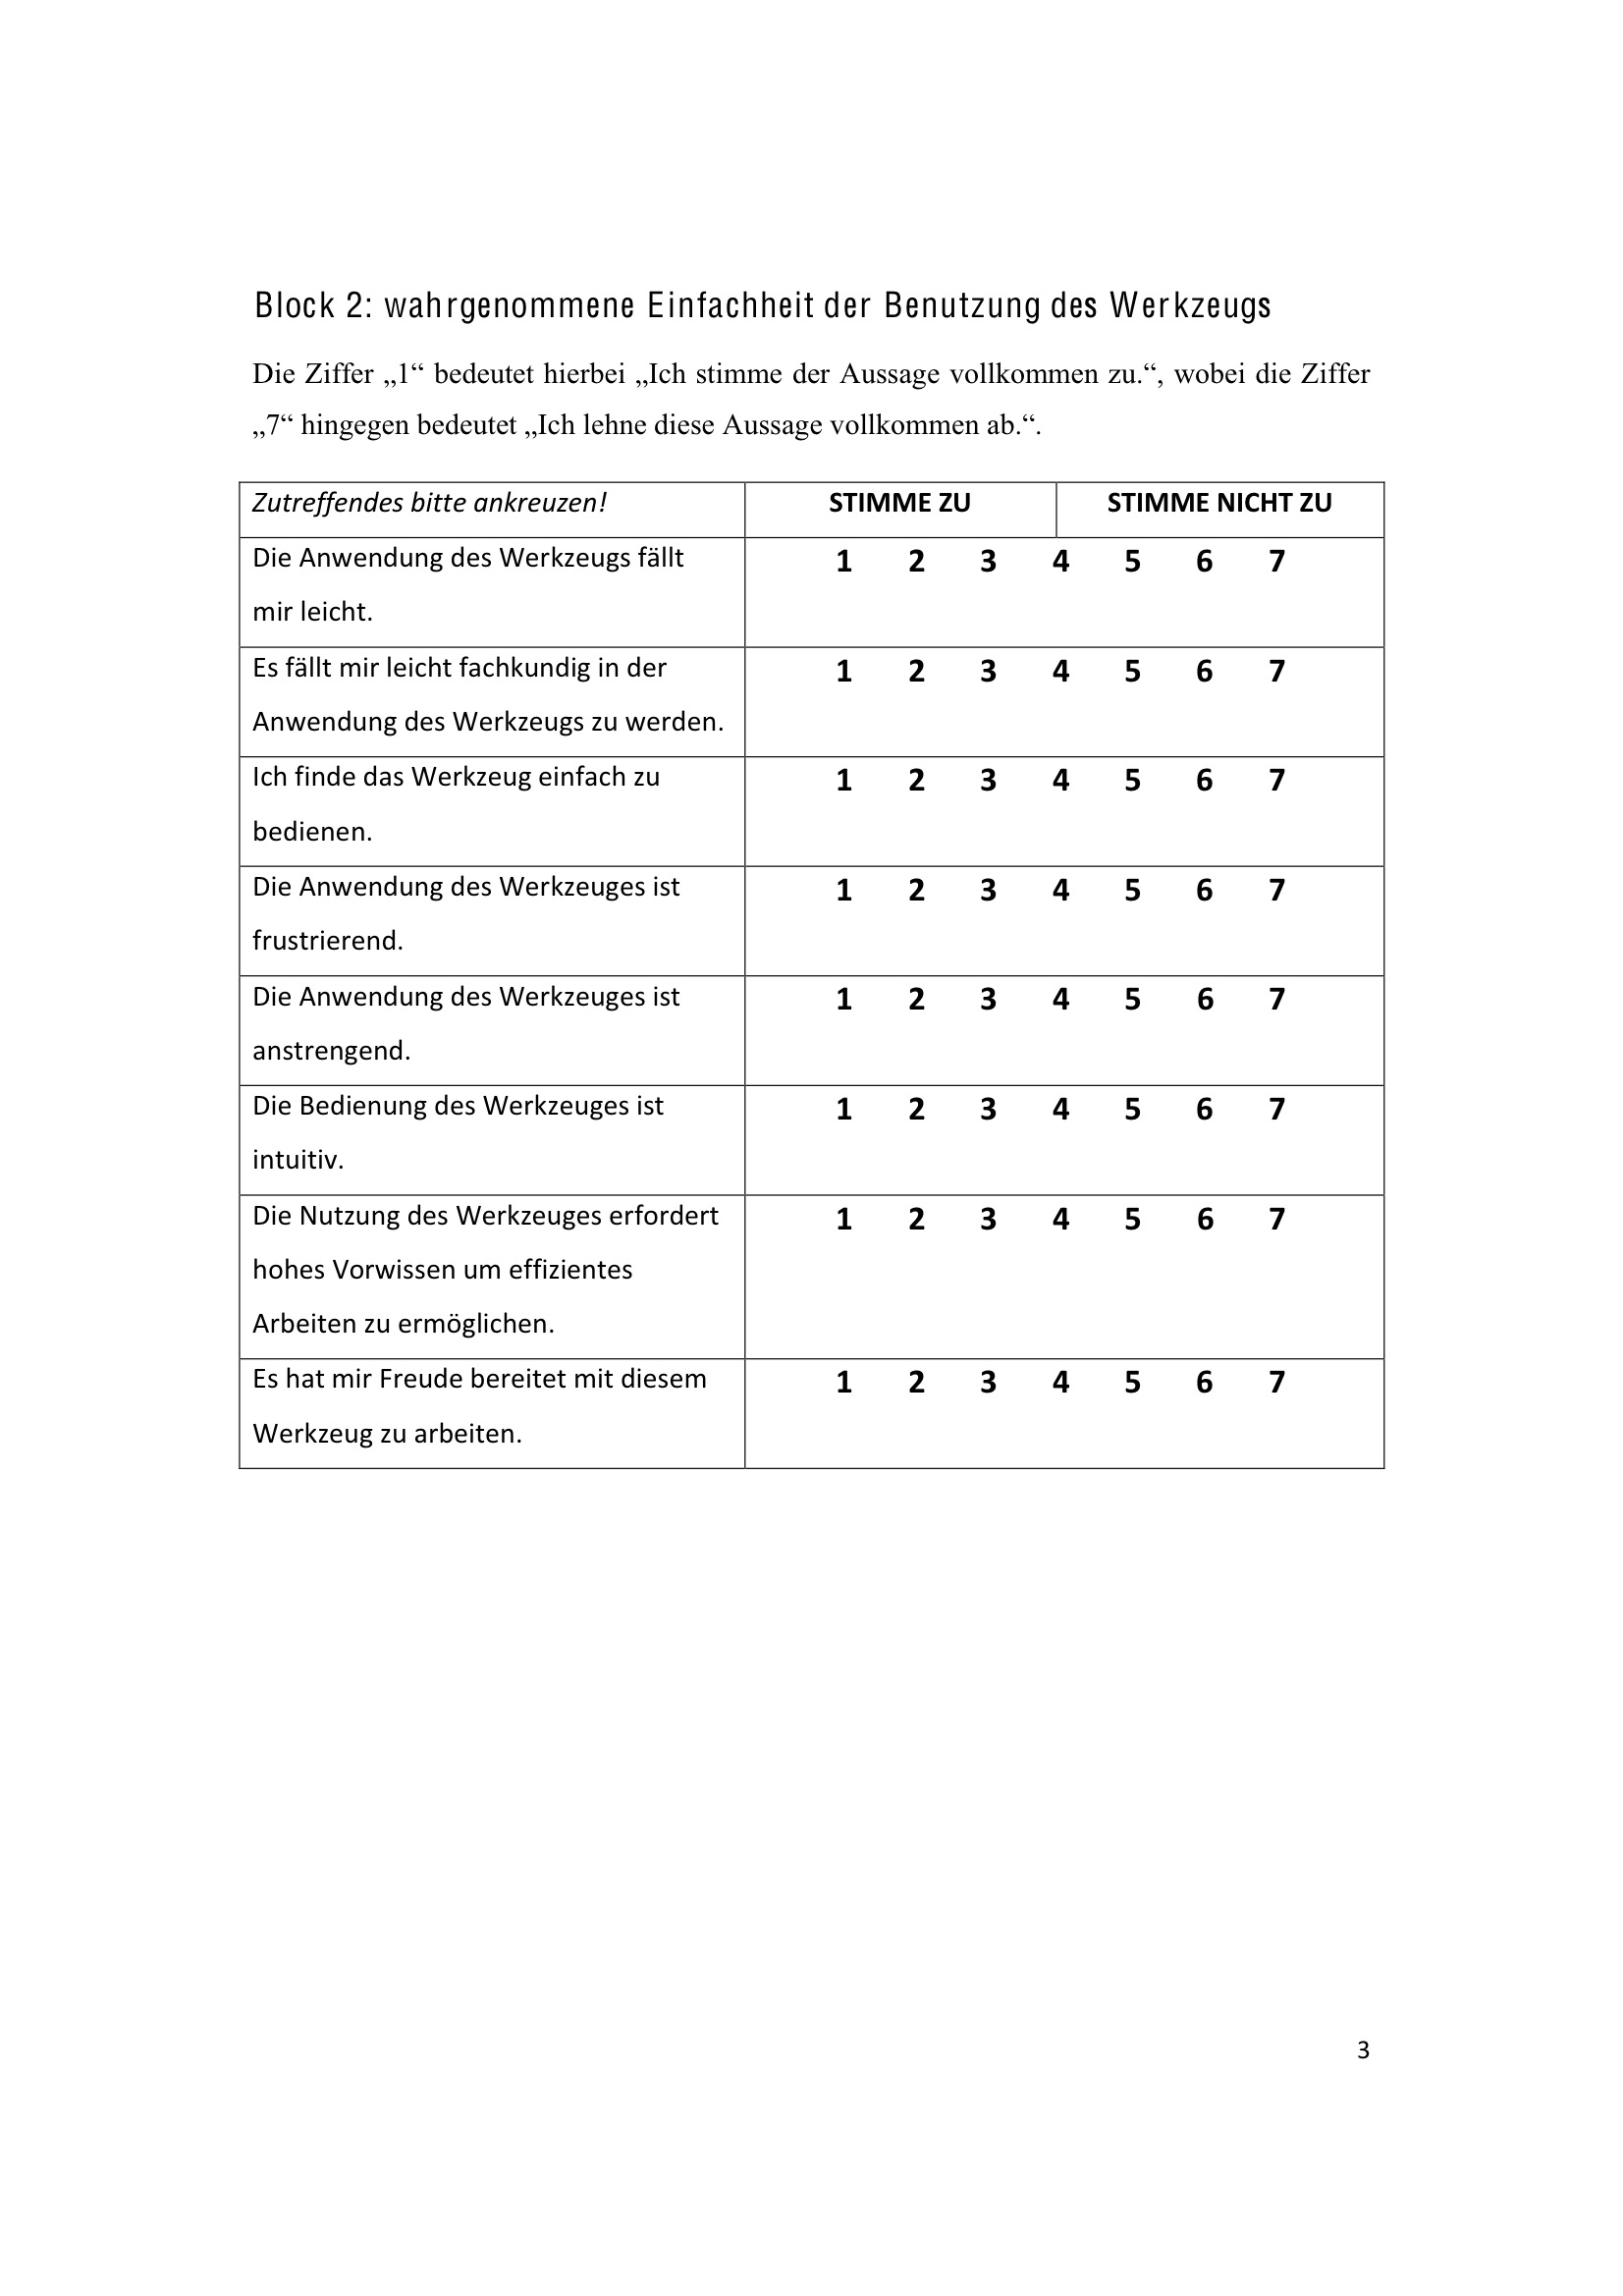
\includegraphics[width=0.9\textwidth]{img/AnhangEmpirie/fb5-03.jpeg}%
	}
	\caption{Fragebogen für Evaluierungsblock 5 - Seite 3}
	\label{fig:img_AnhangEmpirie_fb5-03}
\end{figure}

\begin{figure}[htbp]
	\centering
	\fbox{%
		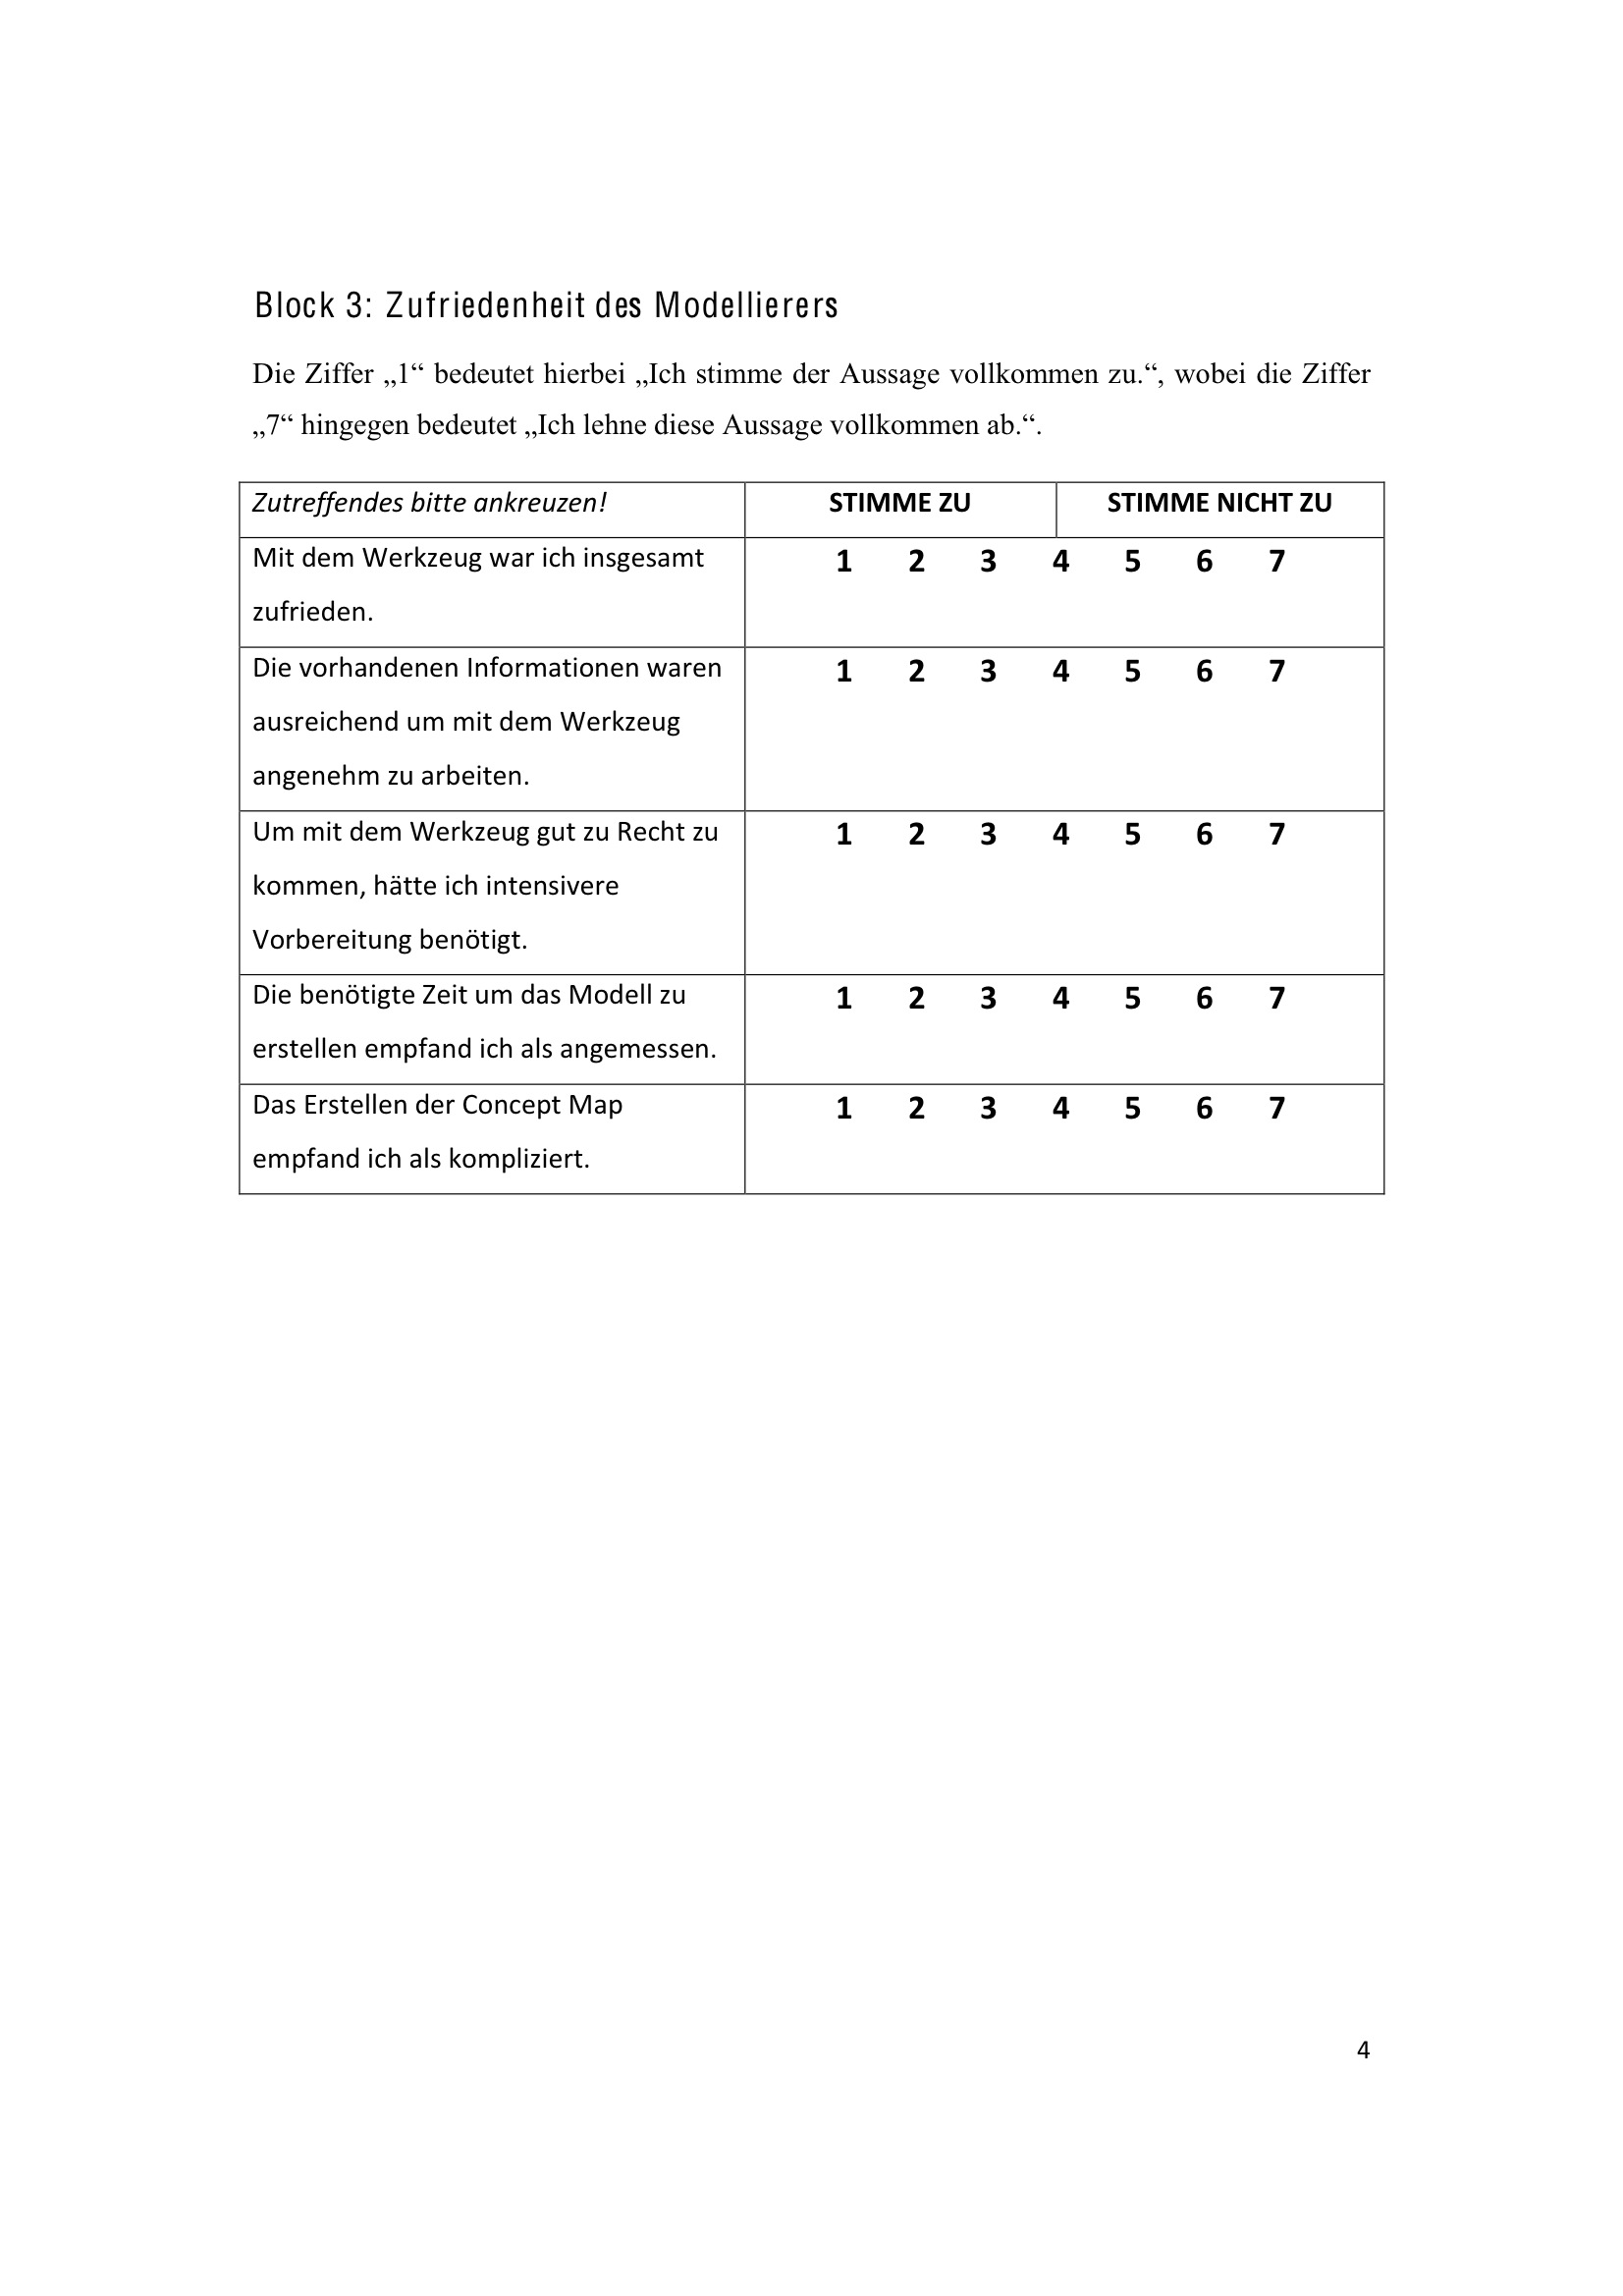
\includegraphics[width=0.9\textwidth]{img/AnhangEmpirie/fb5-04.jpeg}%
	}
	\caption{Fragebogen für Evaluierungsblock 5 - Seite 4}
	\label{fig:img_AnhangEmpirie_fb5-04}
\end{figure}

\begin{figure}[htbp]
	\centering
	\fbox{%
		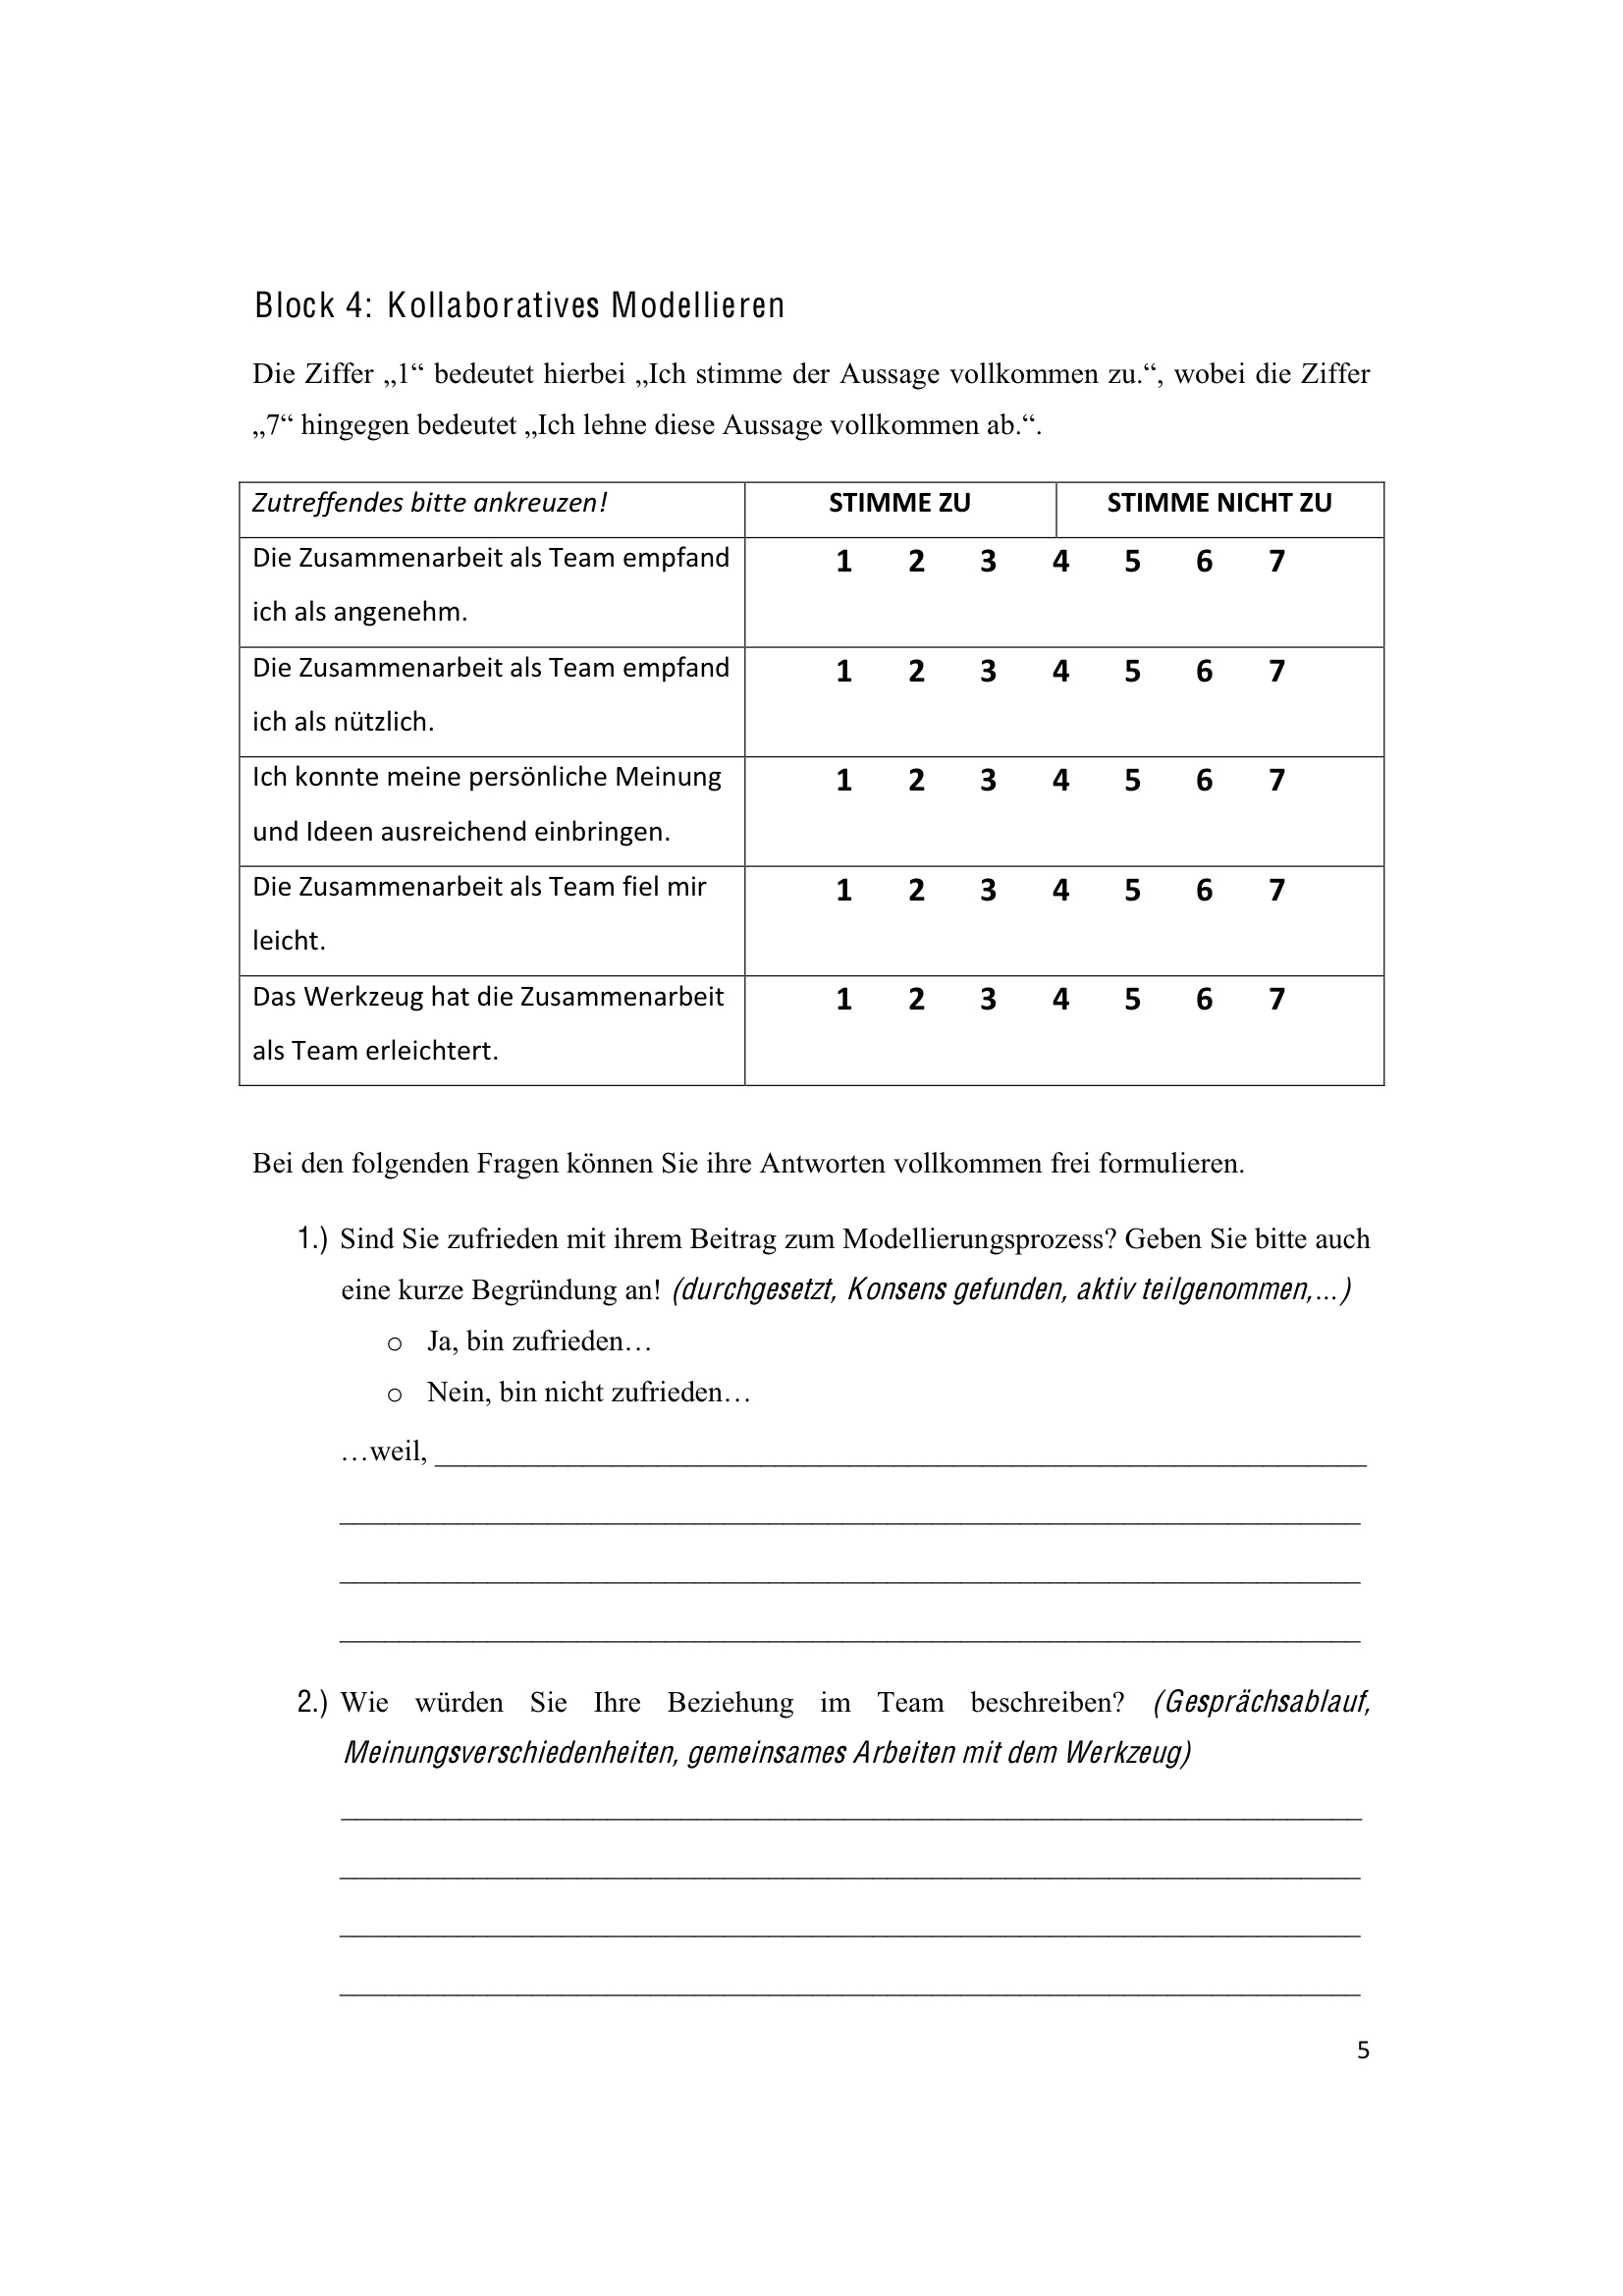
\includegraphics[width=0.9\textwidth]{img/AnhangEmpirie/fb5-05.jpeg}%
	}
	\caption{Fragebogen für Evaluierungsblock 5 - Seite 5}
	\label{fig:img_AnhangEmpirie_fb5-05}
\end{figure}

\begin{figure}[htbp]
	\centering
	\fbox{%
		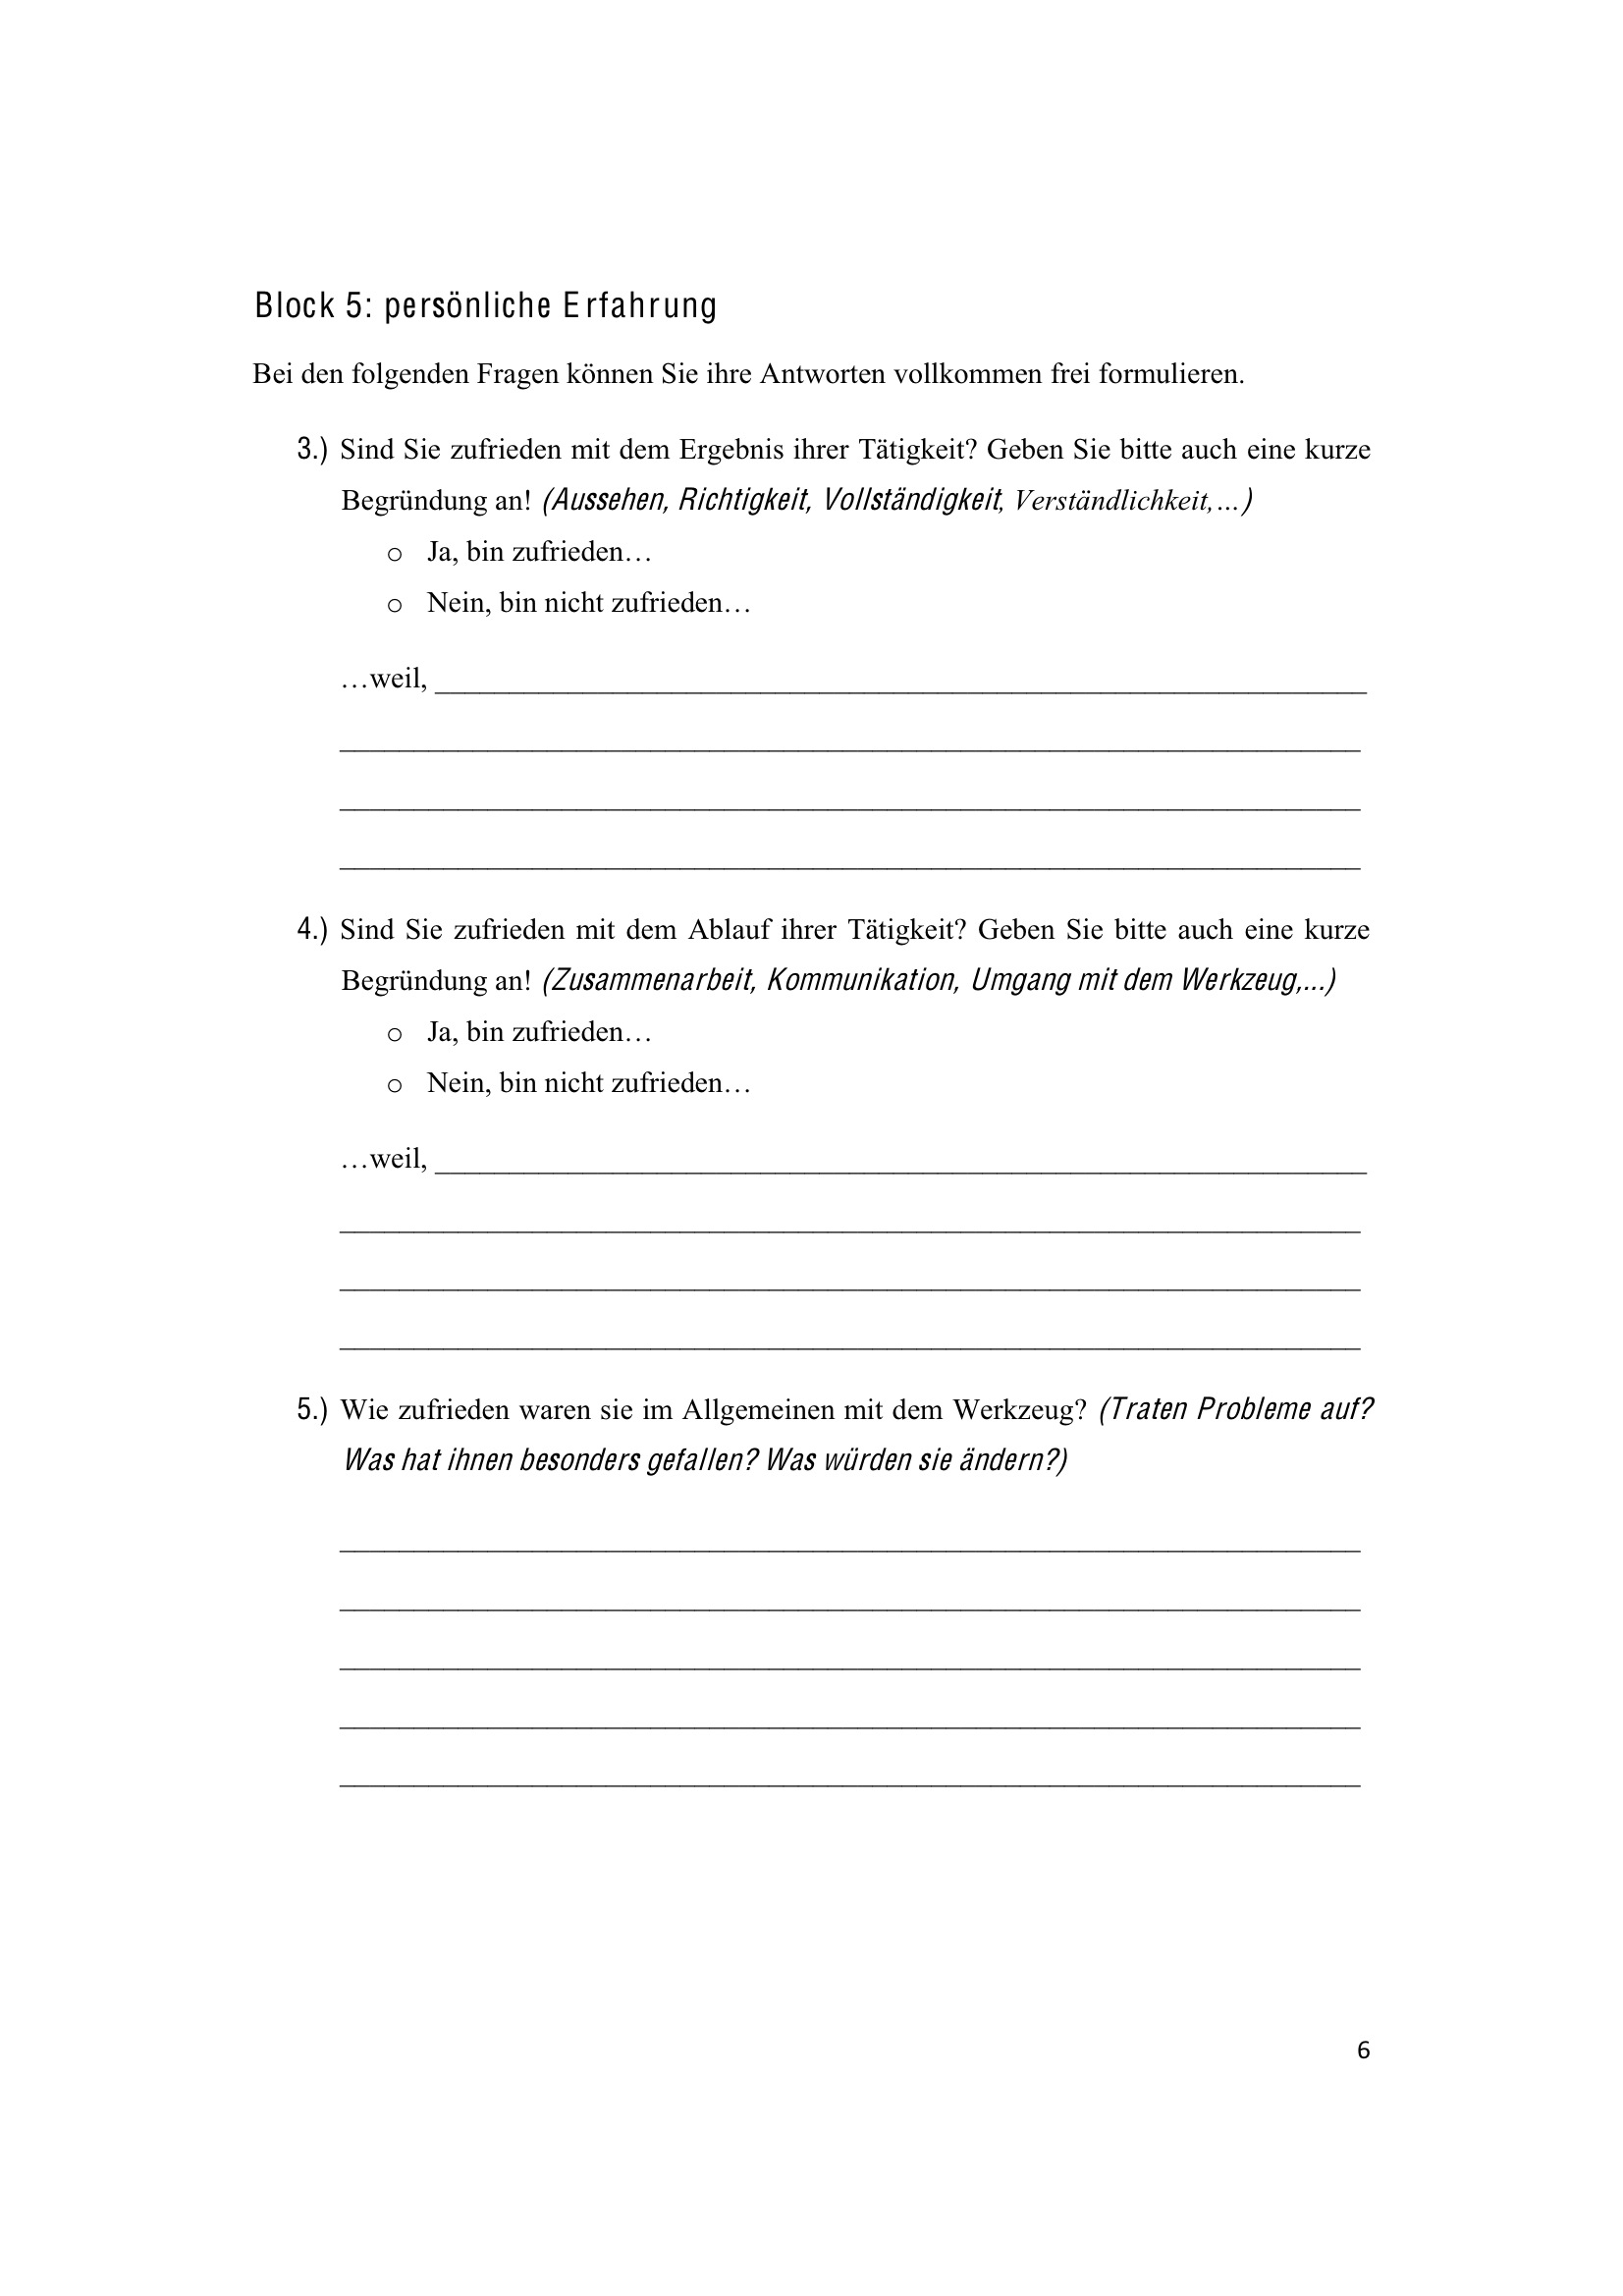
\includegraphics[width=0.9\textwidth]{img/AnhangEmpirie/fb5-06.jpeg}%
	}
	\caption{Fragebogen für Evaluierungsblock 5 - Seite 6}
	\label{fig:img_AnhangEmpirie_fb5-06}
\end{figure}

\begin{figure}[htbp]
	\centering
	\fbox{%
		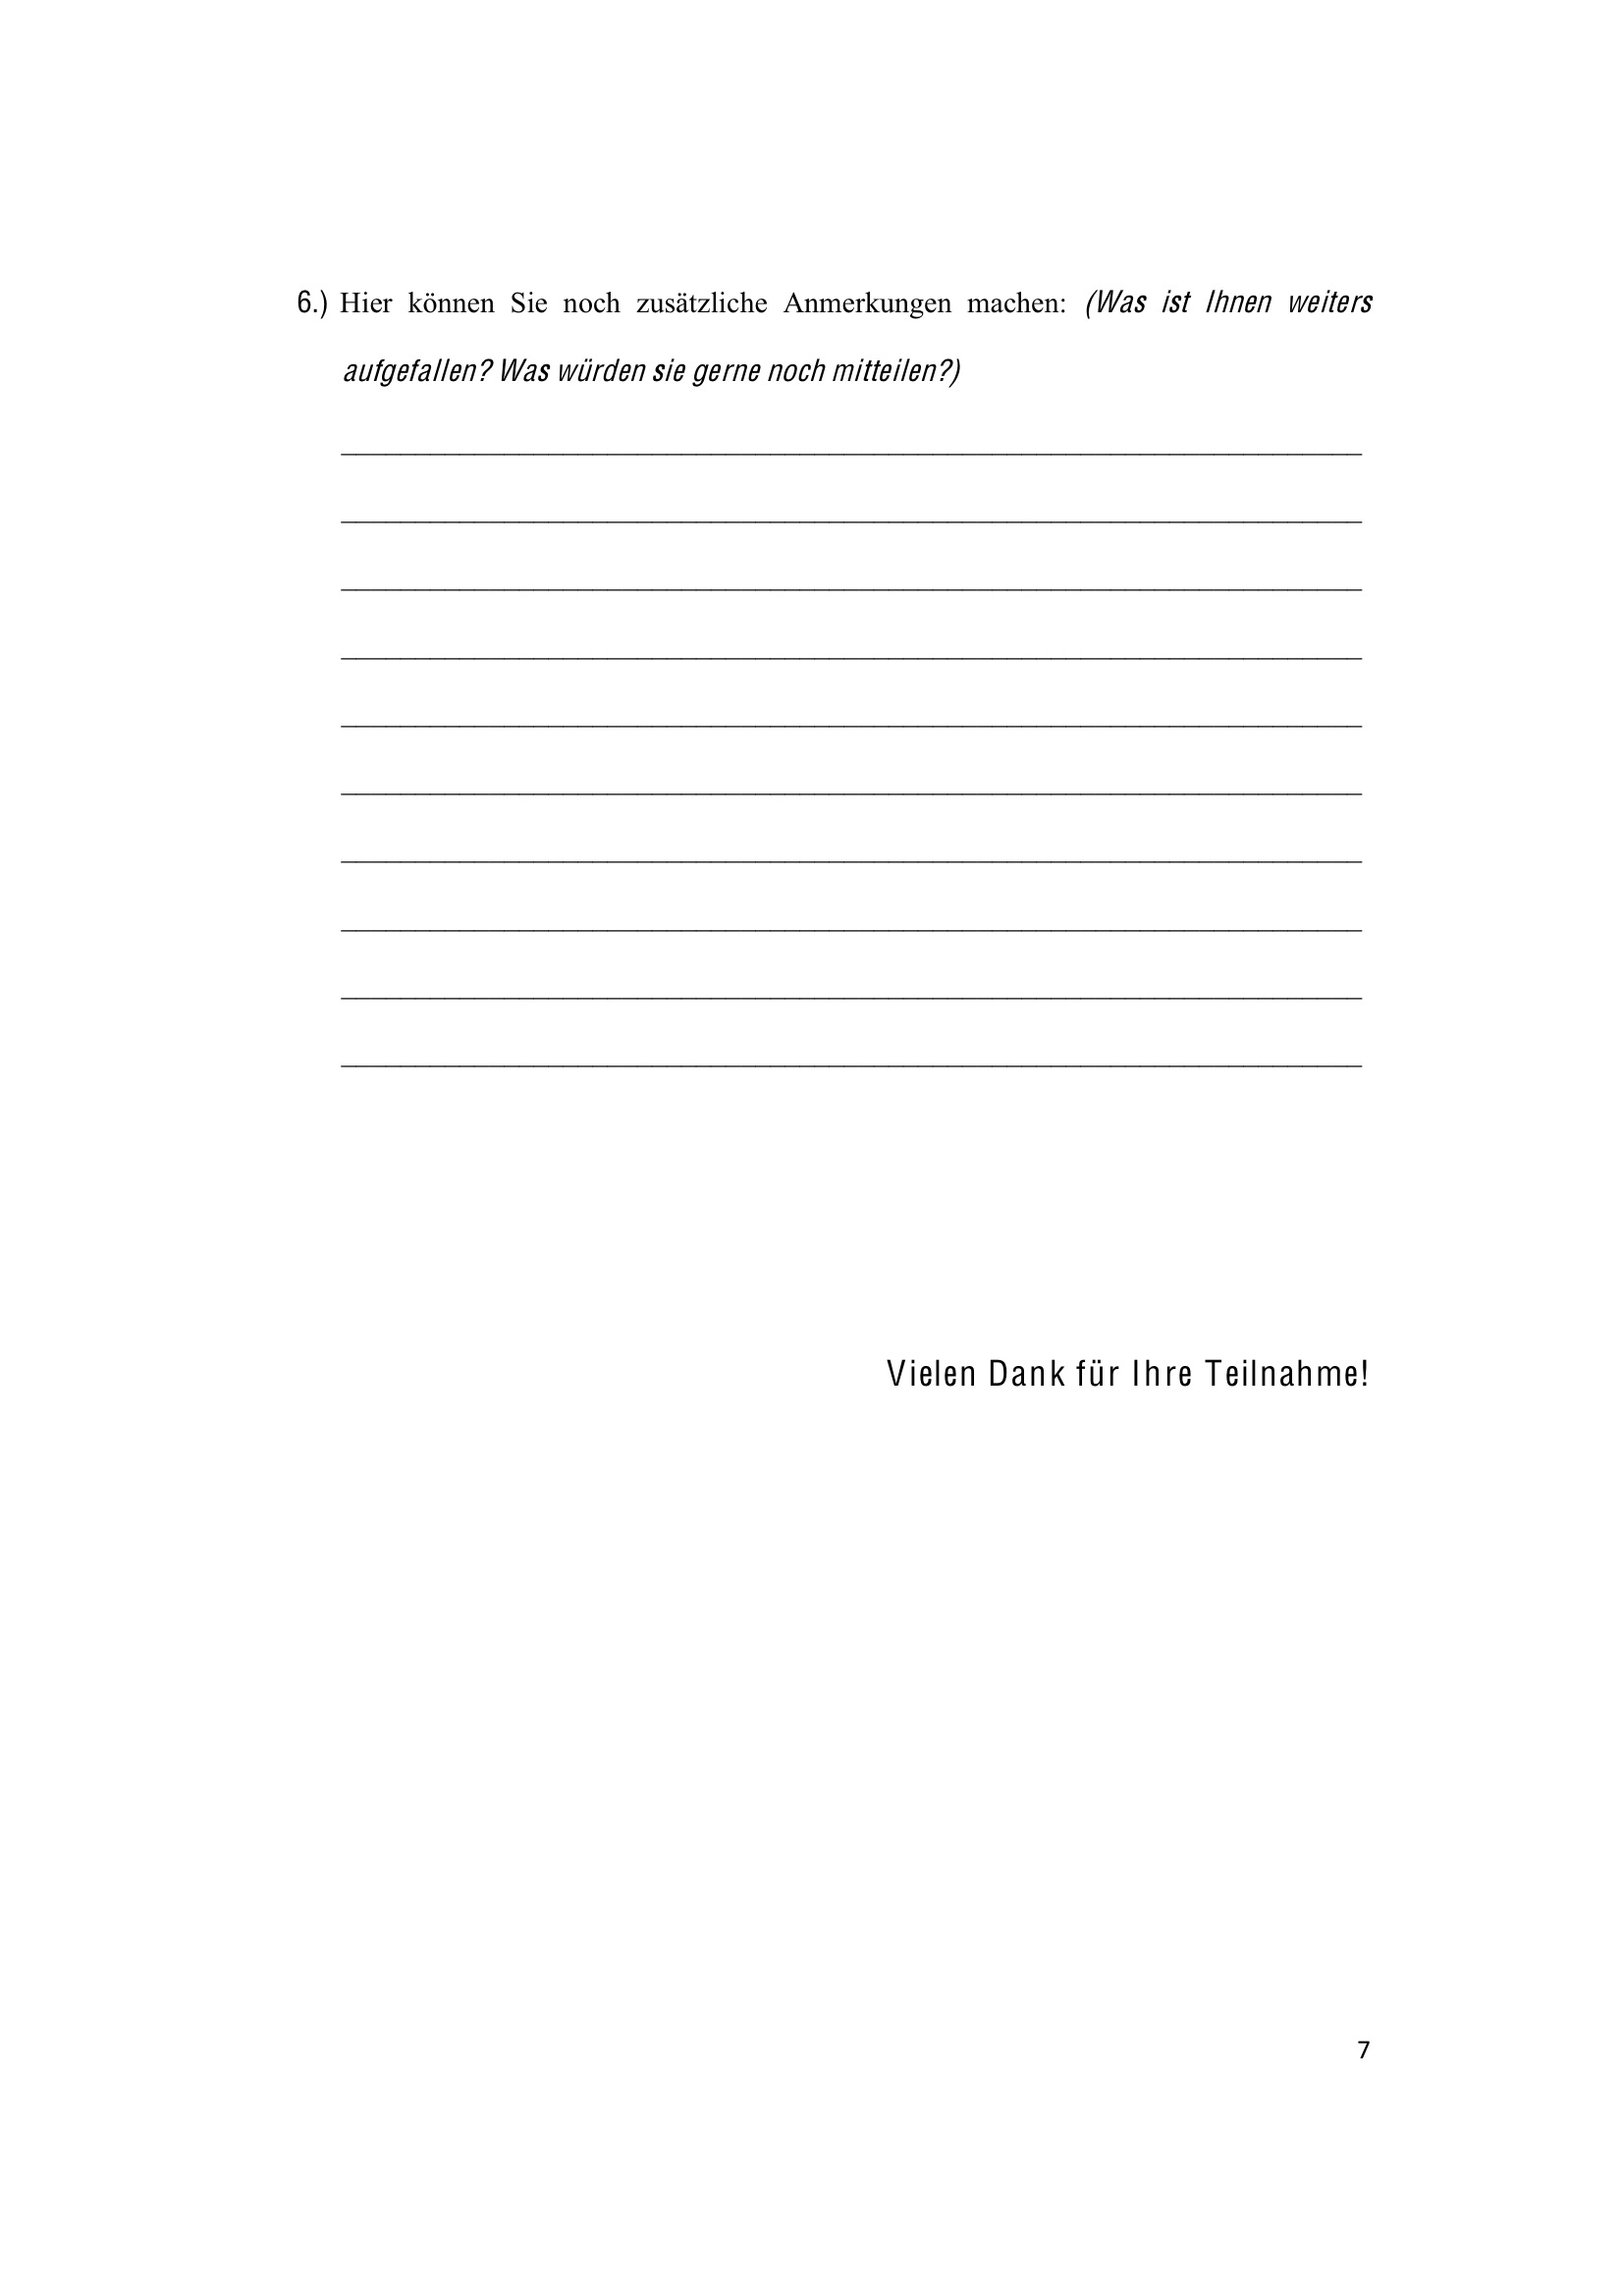
\includegraphics[width=0.9\textwidth]{img/AnhangEmpirie/fb5-07.jpeg}%
	}
	\caption{Fragebogen für Evaluierungsblock 5 - Seite 7}
	\label{fig:img_AnhangEmpirie_fb5-07}
\end{figure}

% section frageboegen (end)

% chapter daten_der_empirischen_untersuchung (end)